\begin{filecontents*}{\jobname.xmpdata}
  \Title{Your Thesis Title}
  \Author{Matthew Asher Bardin}
  \Keywords{comma, separated, keywords}
  \Date{2023-05-31}
  \Language{en-US}
\end{filecontents*}
%
\documentclass[doublespacing]{lsuthesis}
%% To experiment with using a different document class, such as the ``book''
%% class, comment-out the prior line and uncomment the next line.
%\documentclass[10pt,oneside]{book}

%% Specify additional LaTeX packages you need.
%\usepackage{graphicx}
%\usepackage{amsmath}
%\usepackage{amsthm}
\usepackage{pdfpages}
\usepackage{url}
\usepackage{lsutitle}
\title{CYBERINET: INTEGRATED SEMI-MODULAR SENSORS FOR THE COMPUTER-AUGMENTED CLARINET}
\thesistype{Dissertation}
\department{The School of Music}
\soughtdegree{Doctor of Philosophy}
\author{Matthew Asher Bardin}
\degrees{B.M., Stetson University, 2017\\
  M.M., The Boston Conservatory at Berklee, 2019}
\graduationdate{August 2023}


\begin{document}

%% The command ``\frontmatter'' switches to lowercase roman page numbers and
%% unnumbered chapter headings without the word ``Chapter''.
\frontmatter

\maketitle


%% The following ``Copyright'' page is optional. You have inherent copyright
%% on anything you create, even if you choose not to include a copyright
%% notice. But if you choose to also formally register your copyright with
%% the Library of Congress, then a centered copyright notice should follow
%% the title page.
\begin{centeredpage}
\copyright\ 2023\\
Matthew Asher Bardin
\end{centeredpage}  


%% The following ``Dedication'' page is optional.
% \begin{centeredpage}
% The dedication goes here. remove these lines if I don't have one
% \end{centeredpage}


%% The following ``Epigraph'' page is optional.
% \begin{centeredpage}
% \epigraph{All these months I’ve been trying to find find a pattern. Trying not so much to draw hands as gestures. Not so much faces as the expressions of people.}{--Vincent Van Gogh}

% \end{centeredpage}


\chapter{Acknowledgments}

First, I would like to thank my family. Without their continued support, I would not have been able to make it into graduate school, let alone be finishing my dissertation project. Thank you from the bottom of my heart Mom, Dad, Michael, Melanie, and everyone else. 

I would also like to thank my various professors and mentors that I have had the pleasure of working with over the past decade. From building a general approach to music and technology in my undergraduate studies, to finding my passion while finishing my Master’s degree in Boston, to the guidance I received on this project; the advice I have received from these people has helped me to not only build a strong knowledge base, but achieve the confidence to present my work and my art to the world.

Lastly, I would like to thank my cat, Bean. Regardless of whether she was in the way; she always made a spot on my desk to join me while I was writing. When in doubt, I would always defer to her expert opinion on any matters related to eat-scratches, pets, and wet food. Thank you, Bean.

\vspace{10mm}

\begin{center}
    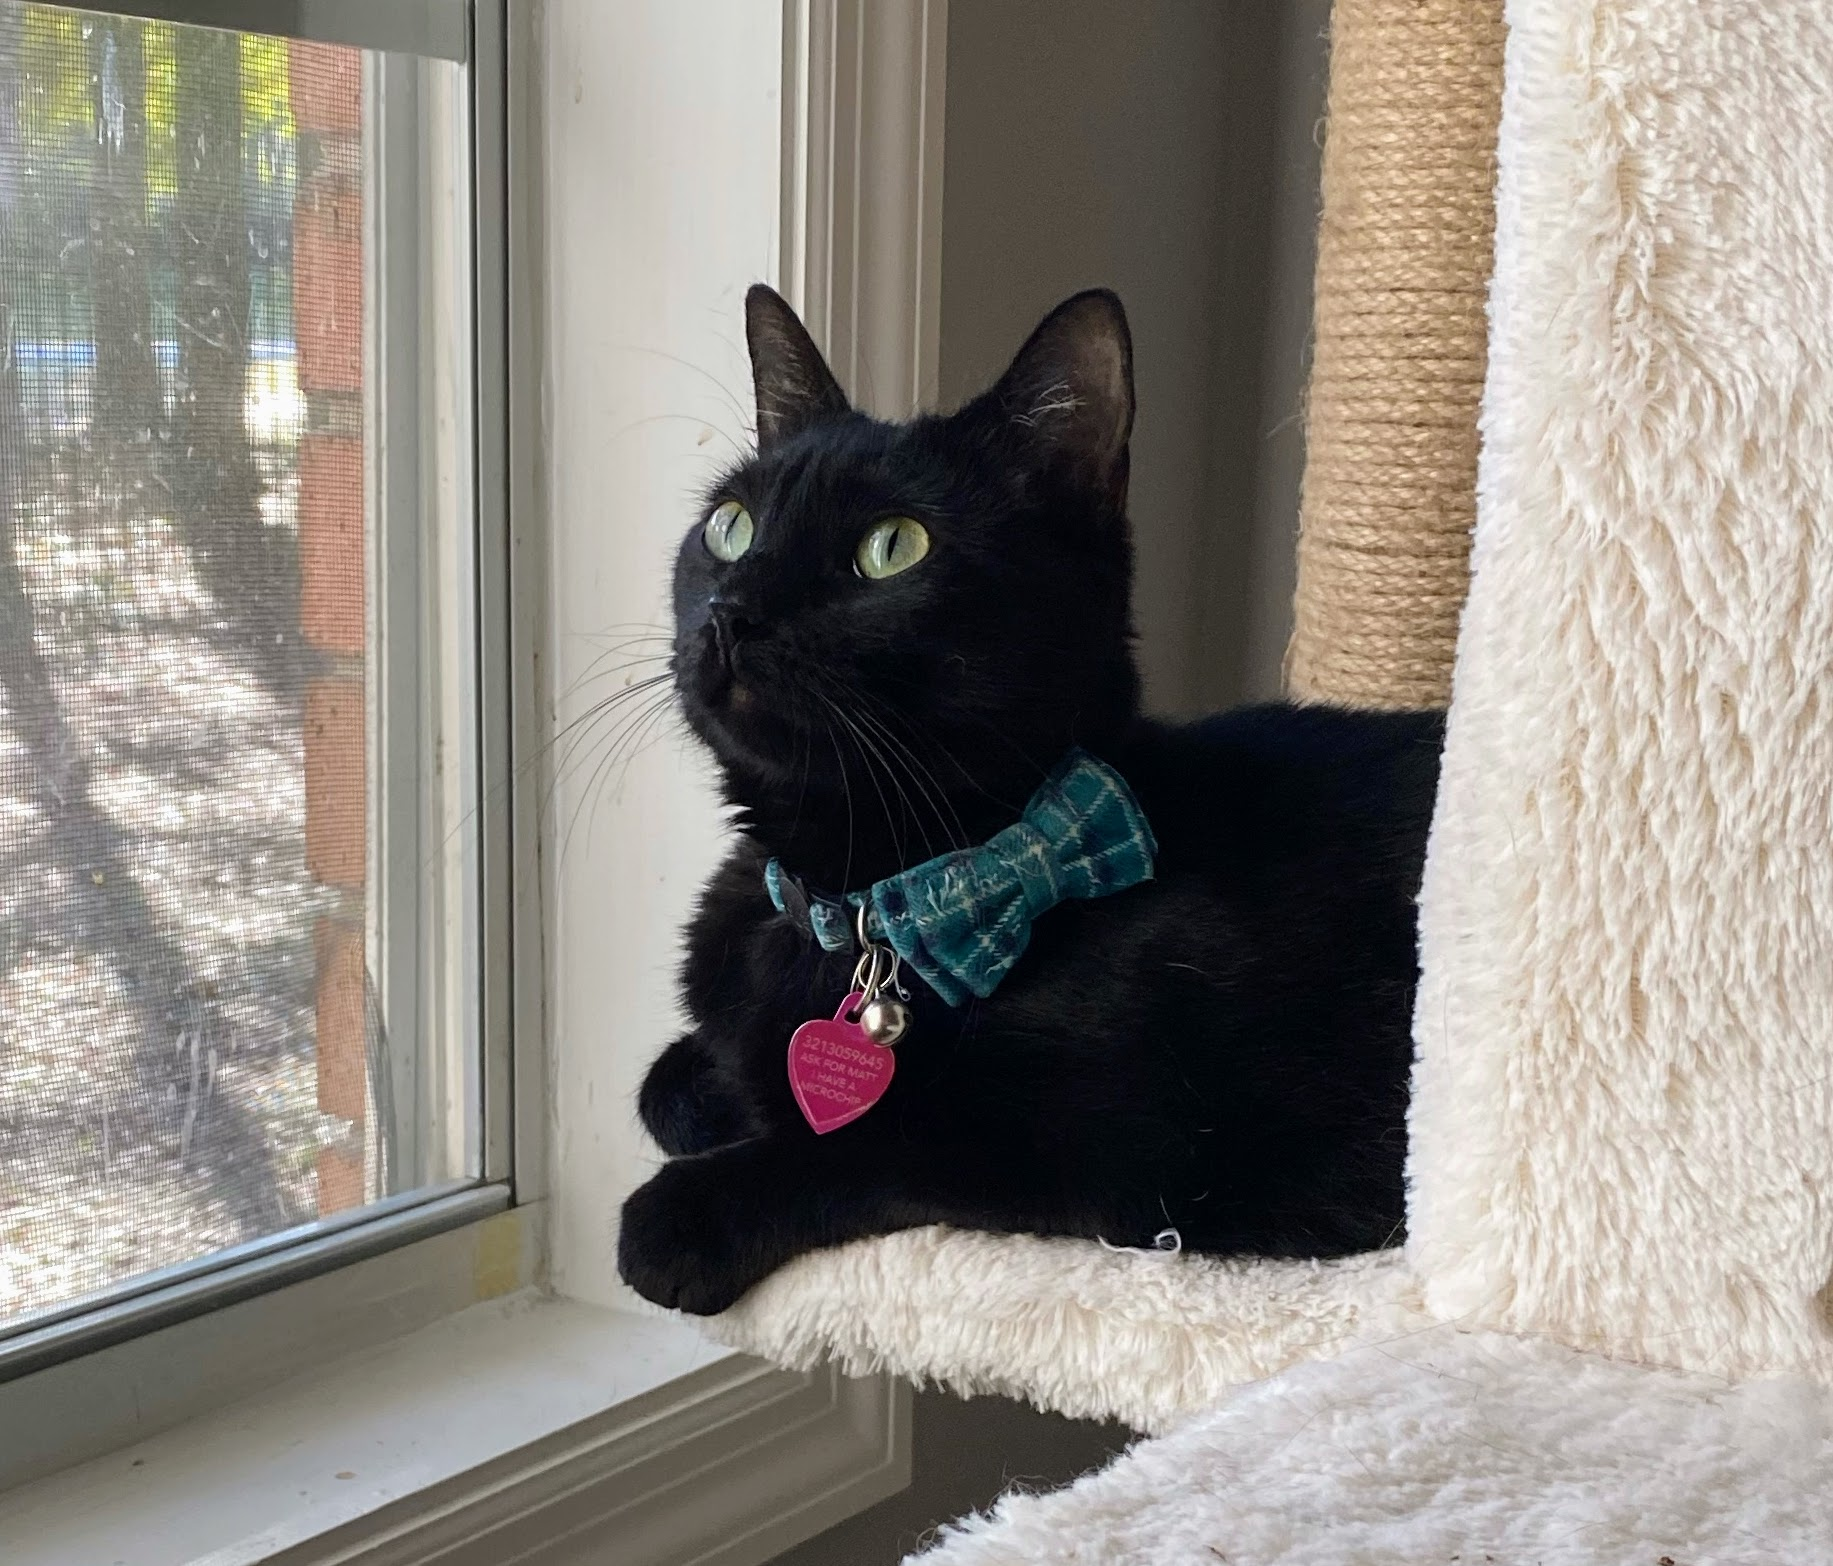
\includegraphics[scale=0.12]{bean.jpeg}
\end{center}



\tableofcontents


% %% The list of tables is optional. Remove the following line if you don't
% %% have tables, don't have many tables, or simply don't wish to have a list
% %% of tables.
% \listoftables


% %% The list of figures is optional. Remove the following line if you don't
% %% have figures, don't have many figures, or simply don't wish to have a list
% %% of figures.
% \listoffigures


% \chapter{Nomenclature, Symbols, Acronyms}

% The ``nomenclature, symbols, acronyms'' page is optional.


\chapter{Abstract}

% The ``abstract'' is required and is limited to 350 words.

The goal of this project is to provide a method of computer-enhanced performance to the solo clarinetist with minimal interference to their normal performance practice. The end goal is for a performer to be able to be able to seamlessly switch between a traditional performance setting and an augmented one with a press of a button. Towards this goal, the Cyberinet is a hardware replacement for a portion of a clarinet containing a variety of sensors embedded within the unit. These sensors collect various real time data gyroscopic data of the performer and air flow within the instrument. Additional sensors can be connected to the Cyberinet to further expand its capabilities, which allows for the unit to become customizable based on various performance needs. This data is then transferred to a computer via Bluetooth connectivity in order to use the data in any number of potential electroacoustic performance settings. The final portion of this project consists of a collection of Max objects designed from the ground up to utilize the Cyberinet’s data in musical contexts. These Max objects were utilized in the performance of four new compositions for the Cyberinet in late April, 2023 at various locations on LSU's Baton Rouge campus.

%% The command ``\mainmatter'' switches to regular page numbers and
%% chapter headings that include the word ``Chapter''.
\mainmatter


\chapter{Introduction}
\label{chap:intro}

% what and why

The practice of creating augmented musical instruments has been a method of creating new and unique timbres in musical performance for centuries. Some of the earliest instrument augmentations still in use today can be traced back to the early brass mutes of the 16th century. In the mid 20th century, John Cage developed a method for augmenting the possible timbres of the piano to vastly increase its sound-color-palette in compositions such as Sonatas and Interludes. 

The topic of this document, the Cyberinet, serves to create a new augmented instrument similar to Miranda and Wanderly's discussion of the concept in relation to gesture-based controllers. % E. Miranda and M. Wanderly. 2006. New Digital Musical Instruments: Control and Interaction Beyond the Keyboard. A-R Editions, Inc. 
Put simply, these augmented instruments begin with an acoustic instrument that has been enhanced in some way through the use of one or more sensors. The Cyberinet, and these other Augmented Instruments work to collect various data from a performance as well as expand the performer's control of the performance environment. Many times these two goals are combined into a single action by the instrument and/or software.
%  L. Jenkins, W. Page, S. Trail, G. Tzanetakis, and P. Driessen. 2013. An Easily Removable, wireless Optical Sensing System (EROSS) for the trumpet. In Proceedings of the International Conference New Interfaces for Musical Expression (NIME), 352–357

% As computer power has increased over the past 50 years, computer processing has allowed for a more dynamic and varied application of instrument augmentation during live performance. As previously stated, the concept of altering an instrument’s method of performing and potential musical timbres has been around for several decades. In fact, this is a potential important step in the development of new instruments. 
% Several works have been developed over the years towards this goal. Within the past 20 years, the Metasax and the Overtone Violin have been two instruments that fall into this category. These instruments take the mechanisms of performing on a alto saxophone and violin respectively, and build upon it to develop that instrument’s augmentation. The Metasax is built from a regular saxophone with various sensors built into the base instrument. These sensors allow for data to be collected and used to process sounds via an external computer. 

% Unlike the Metasax, the Overtone Violin is built from scratch. This instrument replicates the violin in terms of form and sound production, but contains several internal pickups, sensors, and control buttons built into its form factor. In short, the various buttons can be used to adjust the performance modes and help adjust the data being collected and sent to a USB receiver located on a separate glove that the performer would wear. Bertner has written several pieces and performed in several conferences utilizing this instrument. \textit{Windsketches} (performed 2011) and \textit{Endprint} (2004) are two such compositions.

% Both Of these instruments have something similar between them that this project is working to improve upon. That factor is that the performer must either acquire a completely new instrument or potentially permanently alter their instrument to perform with their augmented capabilities. They also require hard-wire connections in some regard, but this is less of a drawback in the context of this project. While these instruments do base their performance practices off of common instruments, there will have to be some level of re-learning the instrument in order to properly make use of its abilities. 

% The Cyberinet works to be minimally invasive to the performance practice of whomever is using the hardware. It is also designed to be easily added or removed to/from a performer’s instrument, eliminating the need for an additional instrument. Two projects that are designed to be minimally invasive are the MIGSI trumpet and the SABRe multisensor. These augmentations both attach to brass and woodwind instruments respectively. 


% These are all potentially useful, but if the performer does not need or want all of these, then they are stuck paying for the sensors that they will never utilize. The effectiveness of the SABRe Multisensor can be seen in compositions such as \textit{Sails} by Matthias Muller (2018). 
% My project seeks to combine the best aspects from these projects and synthesize them into a new semi-modular design that any woodwind player can utilize. It takes the intention of using traditional performance practice to generate its augmentation, while still being something that can be adapted or easily removed in a performance based on the performer’s needs. My hardware is also something that does not impede the movements of the performer. In terms of form factor, My hardware takes inspiration from artist Pamala Z. when in use, one of her sets of sensors is located on her hands, and responds to various gestures to control her performances. Various iterations of these sensors can be seen in several of her compositions, including \textit{Breathing} and \textit{STEIM} (2007).

% Taking inspiration from the SABRe, The Cyberinet's main hardware will be located on the instrument itself. This device will contain the majority of the sensors, batteries, and transmitters. To help with this, the instrument’s mouthpiece and barrel will be 3D printed as a housing for the embedded sensor, which will transmit its data via Bluetooth to a nearby computer.
% Additional sensors can be connected to this unit via USB-C cables. These modular units are designed with the Pamala Z influence in mind. These sensors can be attached to various points on the body, instrument, or performance environment, and are intended to be easily adaptable for any performance setting.

% Optional buttons can also be attached via wire to allow for additional performance control if desired. The wires connecting the optional units and the main hardware are all that is required for the Cyberinet. All of the data is wirelessly sent to the paired control computer. Where it will be utilized to augment the instrument sound and other elements.

\chapter{Defining the Cyberinet}
The idea of augmenting an instrument has been around for almost as long as instruments themselves. In the modern sense, an augmented instrument can be defined as any acoustic instrument that has had an increase in functionality due to additional, usually electronic, additions to the instrument. It is important to note that in order to be an augmented instrument and not something completely new, the original functionality and capabilities of the original instrument remain intact.\cite{miranda_Wanderly_instrumentControl_2006} For example, an electric guitar can still function as a guitar even when not utilizing the built in amplification.


\section{Augmented Instruments}

\subsection{Pre-20th Century Instruments}
In many contexts, the idea of augmenting instruments is viewed as a relatively new practice. While there has been an increase in the number of augmented instruments, especially those with electronic and computer-controlled augmentations over the past century, the concept of improving the capabilities of instruments proceeds the electrical manipulations by centuries.

To clarify this viewpoint, I have two main examples. The first is the development of brass mutes. By itself, a brass mute serves as an entirely mechanical and removable augmentation for the instrument it was designed for. A trombonist utilizing a mute has a greater range of timbral options when compared to a performer not utilizing a mute. While not the first instance of a mute being used in modern music, the score to Montiverdi's 1509 opera \textit{Orfeo} opens with this distinct timbre.

Moving forward a few centuries sees the development of the clarinet. Beginning around 1700, the clarinet is an evolution of the chalumeau which greatly expanded the older instrument's range.\footnote{Because the Clarinet did not have a strong lower register like the chalumeau, it is considered a new instrument rather than an augmentation. It is the same logic that defines instruments like the basset horn and bass clarinet as separate instruments instead of an augmentation of the clarinet.} Originally only having two keys, in the decades following the clarinet's inception, many mechanical augmentations were developed for the instrument. These augmentations were largely the addition of and improvement to the keys and key mechanisms. The end result of centuries of development is the modern clarinet's current physical shape with 17\footnote{The exact number of keys can vary from 17-19 depending on the specific make and model of clarinet.} keys, watertight seals, and changes in instrument material from the original iteration.

\subsection{20th Century Instruments}
During the 20th century is when a large number of augmented instruments begin to be developed. This is due in no small part to the development of audio amplification and recording during the late 19th and early 20th centuries.


\subsection{21st Century Instruments}
The difference between 20th and 21st century augmented instruments is ambiguous at best. Electrical augmentation is still prevalent in the practice, but as the components become smaller and more affordable, an increase in the number of instruments can be seen. %site this claim
Likewise, as computers increased in power, their usage to both locally and remotely control computer augmentation has also increased. While all of the instruments yet-to-be discussed in this document were created in the 21st century, the use of computers % how to define this group of instruments. I like 21st century less as a gouping

\subsubsection{MIGSI Trumpet}
The Minimally Invasive Gesture Sensing Interface, or MIGSI Trumpet is an augmented instrument designed to work with the ergonomics and performance practice of the traditional trumpet\cite{reid2016}. Towards this goal, creator Sarah Belle Reid developed a collection of sensors that fit seamlessly into the form factor of the trumpet. These sensors work to capture control data such as valve placement, instrument position, etc. and send it wirelessly to a computer.

Where the MIGSI is similar to the Cyberinet is in its goals of form factor. The entirety of the MIGSI augmentations are located to match the form of a standard B-flat or C trumpet, and is placed at the instrument's center of gravity to minimize fatigue from the extra weight. While not as streamlined as the MIGSI trumpet, the Cyberinet's sensors are located in a similar location in relation to the design of the Clarinet.


\subsubsection{Music Written for MIGSI Trumpet}

% DO I WANT TO DO THIS OR ANOTHER PIECE? MAKE SURE IT MATCHES THE MUSIC REFERENCED EARLIER IN THE DOC

Ried, has created several improvisations utilizing the apparatus, and written several compositions such as Consider (2017).

Here we will discuss \textit{Pocket Fig} for the MIGSI Trumpet, written by Sarah Belle Reid\footnote{A performance video of \textit{Pocket Fig} can be found at \url{https://www.youtube.com/watch?v=5szWkbVjYxg}}. In this work, Reid utilizes Force Sensitive Resistors as well as Infrared sensors to collect data related to the valve displacement on the instrument. This data is then wirelessly sent to the computer to control a Max patch's granular synthesis processing.

\subsubsection{SABRe}

The SABRe is another sensor array that is designed to work with various woodwinds. The unit straps onto the instrument and can be used to collect airflow and position data to be wirelessly sent to a control computer. While effective and easily removable, this particular device offers a relatively limited amount of usable parameters which can be utilized in an augmented instrument.


% make this section smaller. place after discussing the Cyberinet? if so, where?
Of the discussed instruments, the SABRe is a system of sensors that is the device most closely related to the Cyberinet. Specifically comparing the two devices, we can see clear pros and cons to each.

\textbf{SABRe:}

\begin{itemize}
    \item Pros: small, completely wireless, easily removable.
    \item Cons: no modularity, cost.
\end{itemize}

\textbf{Cyberinet:} 

\begin{itemize}
    \item Pros: integrated within the instrument, expandable with add-ons, relatively inexpensive to produce, open source-components.
    \item Cons: less easily removable, some wires involved.
\end{itemize}

The core units of both devices contain a similar array of sensors. In fact, the SABRe was an inspirational starting point for the development of the Cyberinet. Both devices have a main unit containing the following sensors:

\begin{itemize}
    \item Gyroscope
    \item Accelerometer 
    \item Differential Airflow Pressure
    \item Temperature
\end{itemize}

From the similar sensors between the two different devices, one can infer a similar usage case as well. Both of the SABRe and the Cyberinet are add-ons for a clarinet. By being attached to the instrument, the sensors collect the data they are designed to collect and transmit it to a nearby computer.

The goal of the SABRe is to provide augmentation features to performers, regardless of their technical abilities\cite{Schiesser2012}.

As well as containing a similar base, the units also allow for an optional use of 2 buttons that can be programmed using the computer. However, it is at this point that the sensors begin to differ. It is the view of the author that the SABRe sensor is generally lacking in two main elements. The first is its lack of additional sensor options. While the included sensors are indeed quite useful for collecting performance data.

\subsubsection{Music written for the SABRe}

Prior to 2023, SABRe had been on a hiatus in terms of development and is currently in the process of designing a relaunch of the system. It is perhaps for this reason that there is a limited number of works for the system, but discussing the reasons behind the hiatus is beyond the scope of this paper.

One piece that will be discussed is  \textit{Sailing}\footnote{The performance of \textit{Sailing} can be found at \url{https://www.youtube.com/watch?v=Eiuacb5nJc8}} by the SABRe's creator: Matthias Mueller.  

In this work, Mueller takes the gyroscopic information from the SABRe to control audio effects in real time. The first one heard is the control of the amount reverb and delay time as the performer moves from right to left. This is followed by triggering a tremolo effect that combines with the clarinet timbre. Due to a lack of a score, it is my best guess from the video that this effect is being toggled on with the buttons located on the back of the instrument. By combing these effects with micro-tonal notes, Mueller is able to create a unique sound world easily and effectively.

Mueller also utilizes a pitch shifting effect, but it is unclear if it is created as a unique harmonizing effect, or is created as a by product of adjusting delay times. The final effect is a little distortion present when the performer reaches the extreme ends of the gyroscopic data.

In the future, should a performance score become available, it would warrant more in depth analysis of the performance practice and specific utilization of the SABRe's sensors. However, there is still much that can be learned with Mueller's performance video. It can be seen that Mueller clearly focusing on only one or two sensors present within the SABRe: Gyroscope and Buttons. By focusing on a smaller subset of the sensors, it allows Mueller to allow the capabilities to the system to stand out. It becomes very clear what the correlation between the clarinetist's physical position and the timbres being created are.

Mueller's utilization of the button is worth bringing up individually. in \textit{Sailing}, Mueller is using this button to trigger a tremolo-like effect to be applied to the clarinet's signal. Unfortunately without the software patch or score the fine details of this are left to speculation, but I want to focus on the idea of manually triggering an effect with a button. Unlike a foot pedal, these buttons follow the performer, allowing them to take full advantage of the buttons along with the movement sensors. A performer can access the buttons regardless of their on-stage location. In the Cyberinet compositions discussed later, I utilize a larger-scale use of the main buttons. In \textit{Puzzle of a Park}, the buttons are used to trigger recordings and playback, whereas in \textit{Raindrops on a Tin Roof} I utilize the button's instant binary functionality to cycle through different signal routing and effect presets to alter the tones.

\subsection{Other Similar Devices \& Studies}

FIND THE PAPER I'M REMEMBERING BUT CAN'T QUITE RECALL FOR THIS STUDY, OR ADAPT IT TO FIT ANOTHER PAPER IF IT CANNOT BE FOUND

On its own, the collection of performance data as done in the Cyberinet is not a new practice. However having an easy degree of flexibility and user-friendliness has not been common practice. Generally speaking, most studies or works written that utilize performance data like the Cyberinet have been crested in near-sterile environments with sensors placed all over the performer and their instrument. 

HOW CAN I SIGHT THE PRESENTATION AT THE DMC? LOOK AT HER WEBSITE AND OTHER PAPERS ABOUT THE DEVICES

Even in less academic and laboratory uses, one finds that the devices present are far from accessible. Looking at artist Pamala Z can see many ways that sensors can be utilized in creating new music content. Her music will not be broken down here, but we will look at her sensors. Mainly, Pamala Z utilizes two main sensor units placed on stands and another pair of sensors, although not always at the same time. In terms of design and performance function, the hand-mounted sensors are the closest to the Cyberinet: mounted on the performer, captures natural expressive movements, but can be manipulated for specific effects, controlled by a separate computer via Bluetooth, etc.

Where these sensors begin to differentiate from the Cyberinet is in their inherent accessibility. Pamala Z's sensors were developed by another person (FIND HIS NAME), and were intended to be utilized by specific people in specific circumstances. While the devices could certainly be hacked or their protocols copied to control other, more recent compositions and Max patches, these were never intended for anything other than allowing Pamala Z to create her Art. 

The Cyberinet on the other hand serves to bring all of the sensors and processing capabilities into the hands of as many people as possible. The Cyberinet's form factor is designed to incorporate the electronics with no hassle. Literally the first thing a new clarinettist is thought is how to put the instrument together and hold it. With no external wires (not including the optional expansions), a beginner would be able to utilize the hardware once they have adjusted to the weight. While Pamala Z's sensors are designed to work in specific scenarios and in specific compositions, the Cyberinet is designed as a performance and composition tool for the ground up. The included software bundle includes both examples of composed music for the Cyberinet as well as a collection of objects needed to quickly receive and process sounds in the Max programming environment. 


\section{Cybernetics}
In addition to being an augmented instrument, the Cyberinet utilizes cybernetic principles in its design and intended uses. To better understand this connection, let us look into the concepts of Cybernetics and Cybernetic music.

\subsection{General Cybernetic Concepts}
The concept of modern cybernetics was defined by Norbert Wiener in his 1948 book \textit{Cybernetics: Or Control and Communication in the Animal and the Machine}, which has been republished by MIT press in recent years.\cite{WeinerCybernetics2019} The republished versions contain additional supplementary chapters not included in the original 1948 publication.

%finish book and verify that this is indeed the correct first definition.
In its original context, Cybernetics is defined as \textit{The science of communications and automatic control systems in both machines and living things}. I feel that Weiner's analogy for cybernetics shown below does an excellent job of clarifying what is meant by "automatic control systems".

\begin{quote}
    find original text because this is a paraphrase
    As a captain steers a boat, they see rocks in their path, and turn the wheel to avoid them. Then the captain turns the wheel again to remain on-course. They are not directly adjusting the rudder, and have not planned an automatic course, but rather are acting as a sensor responding to the environment and affecting that system (the boat's movement) based on that system's performance.
\end{quote}

As time progressed, the definition of cybernetics has evolved. Scientifically, the definition is relatively unchanged, still focusing on feedback systems and automated responses, but now also refers to the combination of mechanical an organic components to help achieve this. %citation needed

For example, take the Omnipod 5 system used for diabetics to manage their insulin delivery. This device has the capability to be paired with a constant glucose monitor embedded within the user's abdomen. This sensor will read the glucose levels of the user and automatically adjust the Omnipod 5's insulin delivery rate to compensate for any changes to the blood glucose levels. This system is cybernetic in every sense of the word. It both combines organic and inorganic components, as well as the internal feedback loops to control the blood glucose level of a diabetic in a manner similar to a person without diabetes.

The focus on combining organic and inorganic components comes in no small part from popular culture. Cyborgs were first introduced in science fiction during the middle o the 19th century and have become a major part of the entertainment industry since then. the word cyborg is a portmanteau of cybernetic and organism, and serves to show the melding of organic and inorganic components to form a new being.

\subsection{Cybernetic Music Practices}
Cybernetic principals have also been utilized in music composition. % fininsh introduction

A selection of composers utilizing cybernetic concepts in their music:

\subsubsection{Herbert Brün \textit{(1918-2000)}}



\subsubsection{Roland Kayn \textit{(1933-2011)}}
German born composer who was heavily inspired by information sciences when creating his unique style of mainly electronic and electroacoustic music.\cite{rolandKaynBio} His earliest works to utilize the cybernetic concepts was \textit{Galaxis} (1962) for a variable acoustic instrumental ensemble and \textit{Cybernetic} (1969) for electronics. These works Incorporated cybernetic principals in what Kayn referred to as being "self-governing".\cite{rolandKaynBio} In the context of Kayn's electronic music, this was present in algorithmic processes which incorporated semi-random calculations. These unpredictable results were then fed back into the system which resulted in unpredictable, autonomous results.\cite{rolandKaynBio}

\vspace{10mm}
\begin{center}
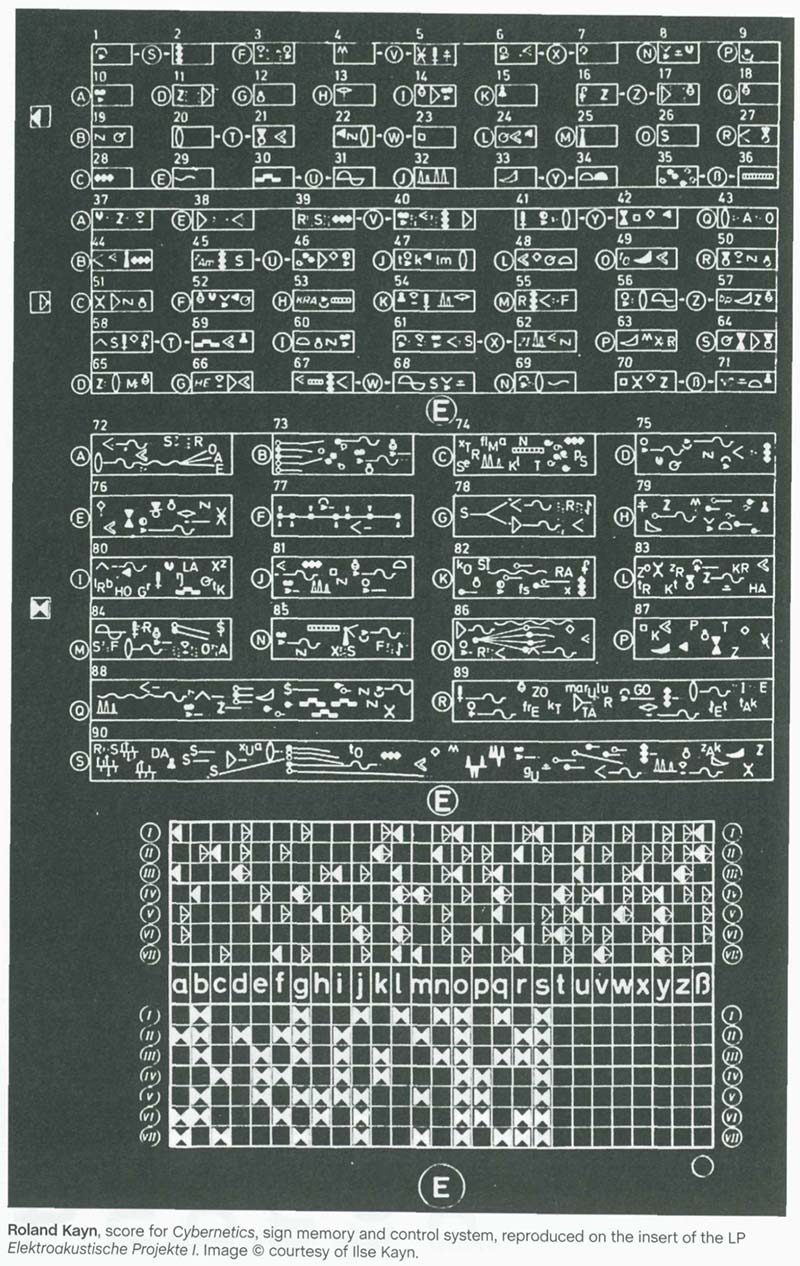
\includegraphics[scale=0.3]{diagrams/kayn_cybernetics.jpeg}
\label{cyberneticsScore}\\
\caption{\textit{Cybernetics} (1969) score}
\end{center}

% show randomsness in the score to make point.
Figure \ref{cyberneticsScore} shows one of Kayn's works, \textit{Cybernetics}.


\subsubsection{Pauline Oliveros \textit{1932-2016}}
An American composer, performer, and educator. Oliveros was a founder of the San Francisco Tape Music Center and pioneer of Deep Listening.\cite{HolmesElectronicMusic2020} Deep Listening is a school of thought at method of listening described by Oliveros as:

\begin{quote}
    ... For me [Oliveros], Deep Listening is a lifelong practice. The more I listen the more I learn to listen. Deep Listening involves going below the surface of what is heard, expanding the whole field of sound while finding focus. This is the way to Connect with the acoustic environment, all that inhabits it , and all there it.

    For others, Deep Listening is a practice consisting of listening and sounding exercises and pieces I and others have composed since 1970. The results are proceeded by a group of discussions in workshops and retreats. 

    Deep Listening is for musicians as well as participants from other disciplines and interests. Previous musical training is not required.\cite{cultureandHumanity2002}
\end{quote}

In short, the idea of Deep Listening itself is a cybernetic practice.\cite{gordosOliverosCybernetics} This is because of Deep Listening's core principle of listening to how you listen. The act of a system responding to itself in a feedback loop is a core concept in cybernetics. In relation to Olivero's music, the concepts of deep listening and cybernetics can be clearly seen in her tape improvisations of the 1950's and 60's. In these works Oliveros along with a variety of collaborators would record themselves improvising, then listen to the recording and discuss what they heard. Following this the group would repeat the process until they were pleased with the results.\cite{gordosOliverosCybernetics} 

This chapter will discuss the context for development of the Cyberinet as well as the process of creating a Cyberinet unit from start to finish.

\section{Design Process}

When developing the functionality of the Cyberinet, the steps defined by Miranda and Wanderley in their book\cite{miranda_Wanderley_instrumentControl_2006} helps to organize and streamline to process. Paraphrased, that process is shown in figure \ref{fig:DMIProcess}. This chapter will follow the process given here and breakdown exactly how the Cyberinet was created.

\begin{figure}
    \centering
    \begin{enumerate}
    \item Determine gestures that will control the instrument.
    \item Determine how to capture the gestures for use within the system.
    \item Define the specific sound creation processes that will be controlled by the sensors.
    \item Map the gesture control data to the desired sound-creation parameters.
    \item: Decide on the feedback mechanisms for the performer to be able to respond to.
\end{enumerate}
    \caption{Digital Instrument Design steps as defined by Miranda \& Wanderley.\cite{miranda_Wanderley_instrumentControl_2006}}
    \label{fig:DMIProcess}
\end{figure}

\subsection{Control Gestures \& Gesture Sensing}
The main control parameter for the Cyberinet is traditional clarinet performance. This process was ultimately chosen in order to help highlight the intended use cases for the Cyberinet\footnote{See Chapter 5 for more information on intended uses of the Cyberinet.}. All of these seek to enhance the clarinetist's sound capabilities without transforming the Cyberinet into a completely new instrument. At its core, an augmented instrument must still retain its identity as the original instrument. \cite[] Towards this goal, a breakdown of a clarinet performance is needed in order to see which gestures are naturally occurring. Other gestures can be added with the additional expansion units, discussed later, but for now we will focus on the main Cyberinet unit.

In a clarinet performance, there are a handful of easily measurable actions that occur. The main ones chosen for the Cyberinet are performer movement, which can often be tied to expressiveness, and performer volume, which can be tied to the volume of air flowing through the instrument. Other parameters exist as well such as determining which keys are being pressed, how hard the keys are being pressed, and which pitch is being produced by the clarinet. While potentially interesting, measuring these data points in real time becomes more problematic due to the necessary placement of sensors and microphones which would potentially impede the performance or alter the instrument into something similar, but distinct from the original clarinet. Because of this, the movement gestures  are the primary focus of the Cyberinet's main unit, followed closely by measuring the air flowing through the horn.

In order to collect the data from the gestures, two main sensors were needed. The final sensors used are discussed in Chapter 3.2, and will be broadly discussed here. When performing the clarinet, the performer generally will pivot or sway horizontally (left-to-right) as they are performing. These motions are the primary focus of the gyroscopic sensors as they are both common to see, and province the largest range of data of the sensors discussed here. Performers can also lean forward or back while performing, necessitating a need for a second degree of motion in the sensor. It is relatively unlikely that a performer will have natural alterations to the vertical height of the instrument while performing, however as shown in Chapter 5, conceptualizing the Cyberinet as a unique instrument opens up the possibility of performance control to traditionally unused actions. Because of this, the Z-axis is also monitored by the gyroscope.

To round out the sensors for the motion gestures, an accelerometer is also utilized in the same three axis measurement. The reasoning for the three dimensions are the same, but with the goal of determining how fast the performer is moving in each direction.

The second main unit sensor is a differential airflow pressure sensor. This sensor was chosen as a way to measure the airflow within the instrument. As a performer creates notes at different dynamics, the volume of air flowing through the instrument will change. By comparing the pressure within the horn with the air pressure outside of the instrument, these values can be easily calculated as a number to utilize in the code.

\subsection{Sound Synthesis}

The Cyberinet is intended to be able to control a variety of software synthesis and control parameters; it does not directly generate sound. Because of this, the software\footnote{Software is discussed in Chapter 4.} is intended to take the sensor data, represent it as a number, then utilize those numbers however they want within the Max programming environment. A handful of Max objects have been created to help facilitate this feature, and for new users to quickly implement the Cyberinet without the need for the user to be an expert in Digital Signal Processing and audio effect programming.

All of these effects are built in Max and utilize common control parameters for the effects. With the exception of any signal input, receive control messages as floating point numbers between 0 and 1.

\subsection{Gesture Mapping \& Feedback Mechanisms}

The Specific gesture mapping is discussed in more detail in the following chapter, but there are a few aspects to discuss here; mainly the idea of determining the most effective parameters to map to. Because of the modularity of the programming, a single gesture can be mapped to anything. This is to create a wide variety in potential outcomes without the need for the performer to learn an equally large number of control actions. When designing the effects, each one has multiple inputs for those who want to utilize them, however each one parameter that offers notable control over the process. These inputs are located immediately to the right of the main signal input for the effect, and include items such as delay times, reverb room sizes, desired harmonizers, and more. Each effect also has a detailed breakdown of its full control parameters, presets, and default values to show off the capabilities of the software both with and without a connected Cyberinet.

In terms of feedback mechanism, this proved difficult to determine in initial planning and prototyping. Ultimately, two main methods were determined to be useful for both the performer and someone working in the Max environment.

On the physical unit are multiple LED's. Several of These are used to indicate that the sensors are all receiving power, but one can be programmed when creating the Cyberinet. At the moment, version 1.3 of the software is utilizing the programmable LED to indicate when the sensor data transmits to the computer. This proves useful for determining whether a connection with the computer is established, and if data should be expected by the computer. In order to avoid blinding the user with LED's they are hidden behind the hardware case of the Cyberinet, and small holes are included to allow for intentional inspection.\footnote{Similarly to the metal grates on microwave doors to allow the user to look in on the food while avoiding the microwave radiation.} As seen later in this chapter, this programmable LED is located close to the airflow sensor's tubes, allowing for the tube ton also function as a light tube to be easily read without needing close internal inspection through the aforementioned holes.

In the software, a handful of options are available to see the incoming data and any errors. If an unrecognized sensors reading or control message is received by any of the software patches, this is returned to the user via both the final outlet of every object, as well as the Max console. Because a user would have to go out of there way to include monitoring within the patch, the main Cyberinet patches able to display all incoming data in the same Max console, , as well as indicate when communication begins and ends. This is useful for monitoring and recording the incoming data, however at times this can be moving to fast to utilize in real time. Because of this, future versions of the software plan to analyze the data and output more helpful notifications such as unexpected data jumps or noise, signal drops, or abnormal ranges of data.



% \section{Audience}

% This is a paragraph inside of a section.

% \subsection{Background}
% \label{sec:background}

% A paragraph in a subsection.

% \section{Citing bibliography entries, figures, tables, and }

% As shown in \cite{latexCompanion}, you
% can reference bibliography entries using the ``\verb|\cite|'' command.
% You can also refer to other parts of the document, such as
% Chapter~\ref{chap:intro} or \S\ref{sec:background}, but letting
% \LaTeX\ handle the numbering. That way, if you move things around, or
% choose a different numbering style, then you won't have to manually keep
% track of the changes.


\chapter{Building the Cyberinet}




% At its core, the Cyberinet contains a small collection of sensors build into the hardware. These include: [list of sensor names]. In addition to these sensors, the unit contain two USB-C connectors on its side. The first one is intended for the button board expansion, which gives the performer access to two buttons positioned on the thumb rest of their instrument. The functionality of these buttons can then be programmed using Max or another audio programming environment. The second USB-C port is designed to connect to a variety of other sensors, allowing for the performer to adjust their setup for whatever is needed for a particular performance. This is the origin of the phrase “semi-modular” in the project title. At the time of writing, one expansion sensor has been created and tested. This is the [figure something out, a mic that will respond to volume and transmit a bang.] Additional expansions have been planned and explored in more detail in the “Further Directions” section of this document. 
% All these chips were selected for their ability to be dropped into the main board without an extensive need for the user to solder many components, and their use of standard 0.1 inch spacing. [fix this sentence]



\section{OEM Sensors}

\subsection{Gyroscope \& Accelerometer}

\begin{center}
    \begin{figure}
        \centering
        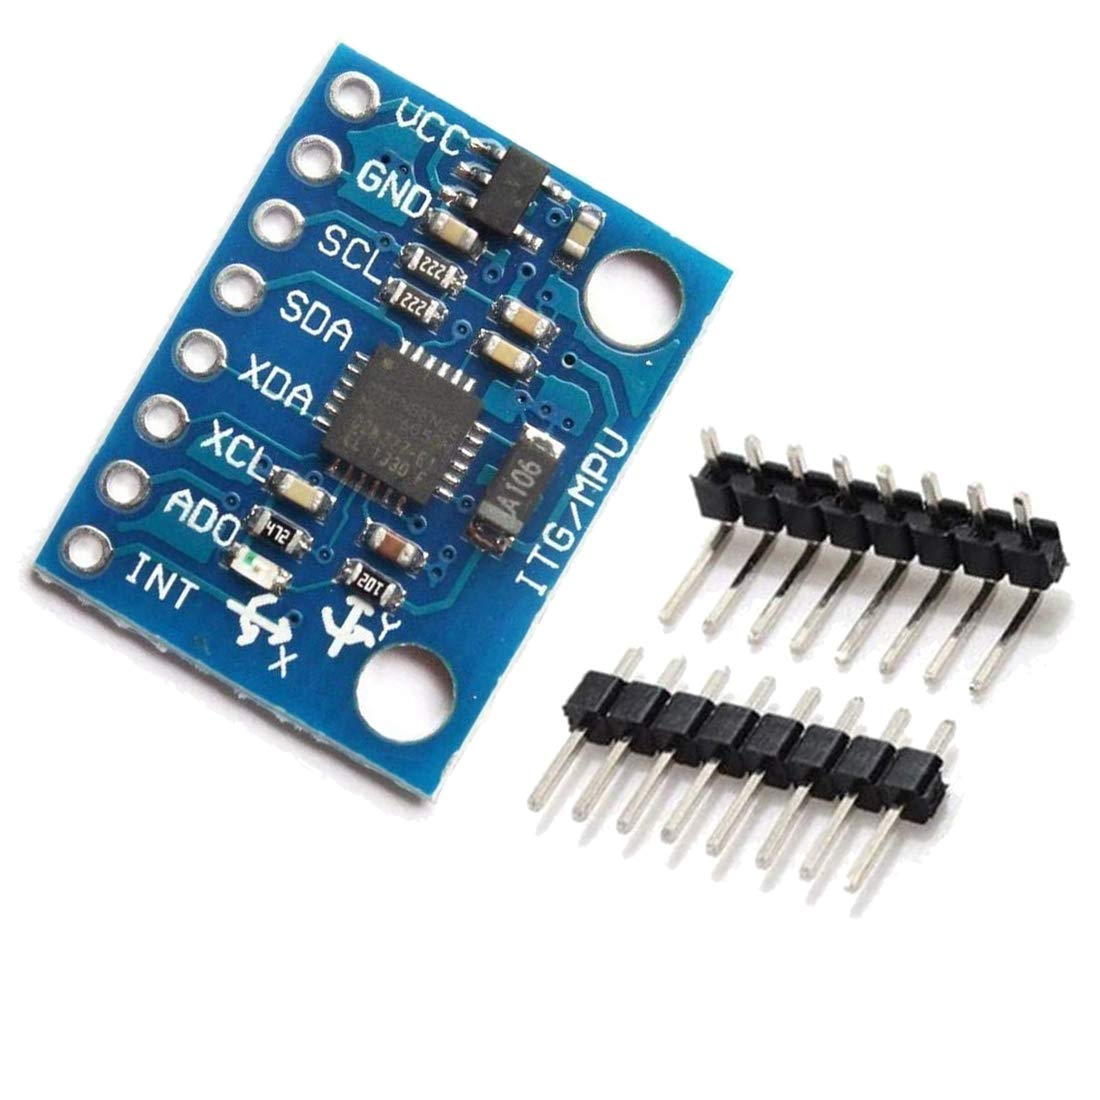
\includegraphics[scale=0.2]{diagrams/oem/6050.jpg}
        \caption{MPU-6050 Gyroscope and Accelerometer}
        \label{fig:6050}
    \end{figure}
\end{center}


\subsection{Differential Airflow Pressure \& Thermometer}

SDP-31
Originally released in [year], this is the newest hardware component in the Bill of Materials. This unit detects differential airflow pressure between two points as well as temperature. Due to the SDP-3X line’s small form factor, the Sparkfun Qwiic connector break out board was selected for simple installation. Two small tubes are attached to the ports and used to measure the air pressure difference between the inside of the clarinet mouthpiece and the outside of the instrument.

\begin{center}
    \begin{figure}
        \centering
        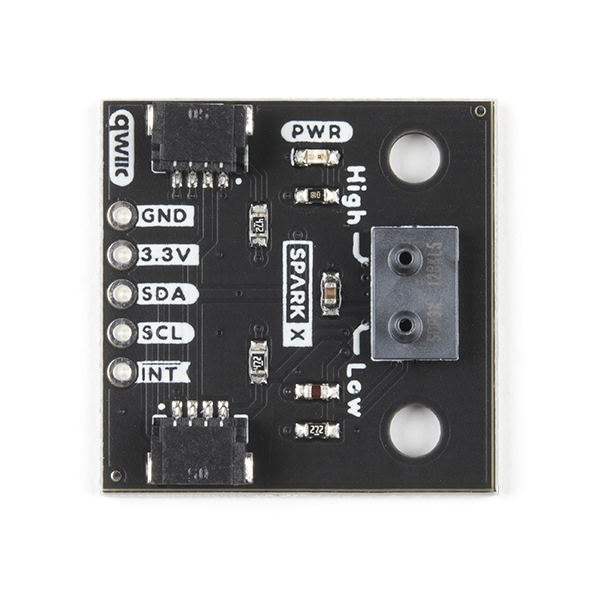
\includegraphics[scale=1.5, angle=90]{diagrams/oem/spd31.jpg}
        \caption{Sparkfun SDP-31 Differential Airflow Pressure Qwiic Connect Breakout Board}
        \label{fig:sdp-31}
    \end{figure}
\end{center}

Because of it’s higher accuracy, the SDP-31’s temperature sensor is utilized over the MPU-6050. Temperature is measured in degrees Celsius.



\section{Controllers \& Power Distribution}

\subsection{Micro-controller}
The Cyberinet contains a variety of useful sensors, however without the micro-controller, they become effectively useless in this context. In order to effectively manage all of the sensors and transmit the data, the Espressif ESP-32 DEVKIT V1 was ultimately selected for use with the Cyberinet. This board was selected for a handful of reasons, including:

\begin{itemize}
    \item Board's narrow size
    \item Large number of ports
    \item Arduino compatibility
    \item Wireless communications
\end{itemize}

The first two items on the list are closely related. While being narrower that comparable Arduino units, the ESP-32 DEVKIT V1 has 30 unique I/O Pins\footnote{Other versions of the DEVKIT have 36 GPIO pins. These boards are incompatible with the PCBs used in the Cyberinet.}. While four pins are dedicated to power distribution and another for the 'enable' functionality (EN), the remaining 20 can be utilized for sensors in a variety of ways. All of this potential functionality is compressed to just under 3 centimeters wide. Because of the ultimate physical design of the Cyberinet unit, having a large amount of accessible pins in a smaller unit was considered ideal. The DEVKIT V1 was preferred over the significantly smaller base chip to increase the simplicity of prototyping, repair, and future changes due to its OEM compatibility, and the popularity of the board among the community. The specific ship dimensions can be seen in figure \ref{fig:esp-32}

\begin{center}
    \begin{figure}
        \centering
        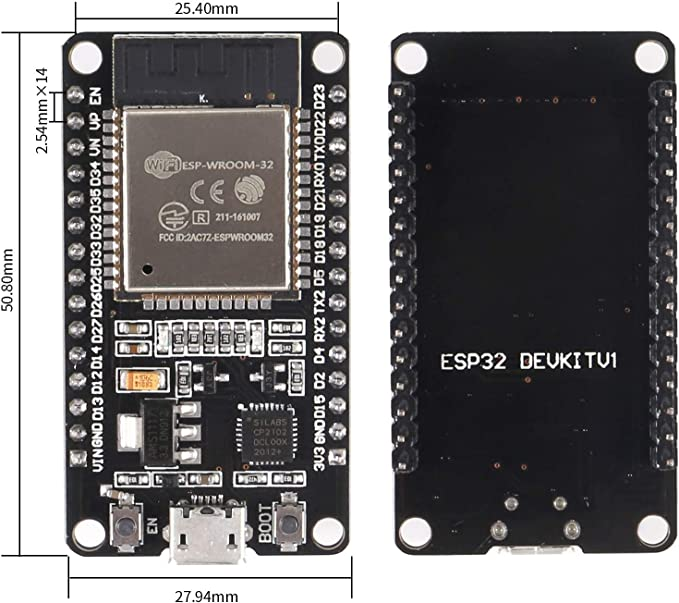
\includegraphics[scale=0.5]{diagrams/oem/esp-32.jpg}
        \caption{ESP-32 DEVKIT V1 micro-controller used in the Cyberinet}
        \label{fig:esp-32}
    \end{figure}
\end{center}

 

Because of the large number of Pulse-Width-Modulation-Controlled GPIO pins, the Cyberinet has the potential for a large number of sensors and expansions, but to help contain the form factor, only a handful are being utilized at any time. We can see the included sensors attached to the pins as shown below. More details about each of the sensors are discussed in each of the following sub-chapters. The labels in the figure below utilizes the pin labels that are printed on the DEKVIT V1. The placement of the shown pins are also shown in figure \ref{fig:esp-32}.

\begin{itemize}
    \item VIN: Power from Battery
    \item GND: Ground
    \item 2: Power LED
    \item 4: Togglable LED
    \item 12: Button 1
    \item 14: Button 2
    \item 21: Gyroscope and Airflow Data
    \item 22: Gyroscope and Airflow Clock
\end{itemize}

Both the Gyroscope and Airflow pressure sensors utilize the same pins. These are the I2C pins on the DEVKIT. More details will be discussed in the chapter discussing the Arduino programming, but it should be noted now that these sensors are able to utilize the same pins because they utilize different I2C addresses. The code is able to access these different addresses in sequence when collecting data.

The code written for the ESP-32 DEVKIT was created using the Arduino IDE and coding language. For similar reasons to the choice of the DEVKIT, this was done for greater accessibility and simplicity in programming. More details about the Arduino Code are discussed later, and the code as a whole is included in the appendices.

The final item from the initial list was the wireless capabilities. The ESP-32 is able to perform serial communications with a connected computer via a micro-USB or USB-C cable (depending on the board version). While useful, the goal of the Cyberinet is to provide affordable instrument augmentation with minimal alterations to the clarinetist's performance practice. Towards this goal, minimizing the number of extra cables was a design concern from the first prototypes. By utilizing the built-in Bluetooth capabilities, the performer is able communicate with the computer easily while meeting this requirement.

The ESP-32 also has WiFi connectivity capabilities which may be involved in a future version, but at the current time is currently not utilized. The DEVKIT is able to support Bluetooth version 4.2 and Low Energy protocols for local wireless communication. This allows for the Cyberinet to easily pair with any computer that it has previously connected to using the BTSerial Arduino library. A code library that brings the normal wired Serial functionality to the Bluetooth functionality.

While not as powerful as the most up-to-date Bluetooth hardware, the DEVKIT's version 4.2 allows the Cyberinet to connect to a computer from up to 200 feet away with a max data transfer speed of 1 Mbps. While these values do fluctuate depending on the performance venue layout, and have a minor impedance from the case of the Cyberinet itself, the performance statistics are still high enough for a large majority or performance areas. This will be discussed more in the chapter discussion the music compositions and performance with the Cyberinet. 


\subsection{Power Distribution}
In order to power the entire system, a lithium ion polymer battery is included inside the hardware. In order to charge the unit, users can utilize the provided USB-C cable and power adapter to the port located on the bottom of the unit. % show pic of charging port


All power distribution for the Cyberinet is handled with a TP-4056 Type C chip, shown in figure \ref{fig:tp5046}. The version containing a USB-C connector was chosen over the Micro-USB connector for two main reasons. The first being a desire for consistent, modern connectors in the device, and the second reason being that this upgraded version allows for both battery charging and distribution. The older Micro-USB chips only allow for battery charging.


\begin{center}
    \begin{figure}
        \centering
        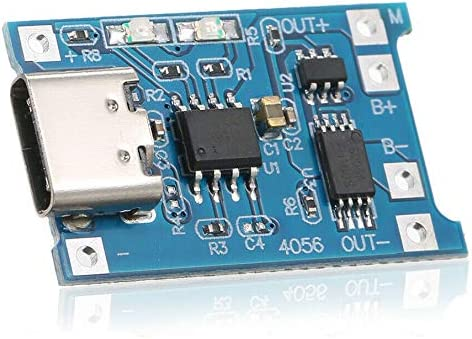
\includegraphics[scale=0.5]{diagrams/oem/4056.jpg}
        \caption{The TP-4056 Power Distribution Chip used in the Cyberinet}
        \label{fig:tp5046}
    \end{figure}
\end{center}

By connecting the battery to the connections labeled B+ and B-, and connecting the Vin and GND pins of the ESP-32 to the OUT+ and OUT- on this board, the Cyberinet is able to receive all required power through the single chip. The power button is soldered into the connection between the battery and the TP-4056, and will automatically power the Cyberinet when activated\footnote{Because of the placement of the power switch, the device will have to be powered on while charging. This can be easily verified by the onboard LED's}. 

When the battery is depleted, it must be connected to a power source via this USB-C port to be able to fuly charge. From an empty charge, the unit can take between one and three hours to fully charge. The exact times can vary depending on the power adapter and whether any additional accessories are connected. 

The battery included is rated for 1200 mAh as an improvement over the 320 mAh battery used for initial testing and prototyping. This size battery allows the Cyberinet to have as much run time as possible while still maintaining the size characteristics of the hardware electronics. The approximate run times are as follows:

\begin{itemize}
    \item Powered on, not connected: 5 hours.
    \item Powered on, Bluetooth connected, no expansions added: 5-6 hours.
    \item Powered on, Bluetooth connected, expansions added: 4-5 hours.
\end{itemize}


It should be noted that the device can also run when connected directly to the wall socket power supply. This will also charge the battery, which, while resulting in yet another wire, can result in an indefinite run time.

% below doesnt actually happen. uncomment when .ino code allows for it to happen
% When the battery capacity becomes critically low, the device will stop transmitting data, however the LEDs may stay on due to residual amounts of electricity present in the system. To avoid accidental drop outs during a performance, it is recommended to fully charge the device prior to any performances to avoid this. When the battery reaches 20\% charge, the red LED on the device will illuminate, and then flash as shown below:

% \begin{itemize}
%     \item 15\%: 1 flash
%     \item 10\%: 2 flashes
%     \item 5\%: 3 flashes
% \end{itemize}

\subsection{Optional Expansion Sensors}
In addition to the built-in sensors, the Cyberinet utilizes a variety of optional expansions that can be implemented as needed to customize the array of sensors. The main expansion unit contains two momentary push buttons and is discussed in greater detail below.

\subsubsection{Button Expansion}

\begin{center}
    \begin{figure}
        \centering
        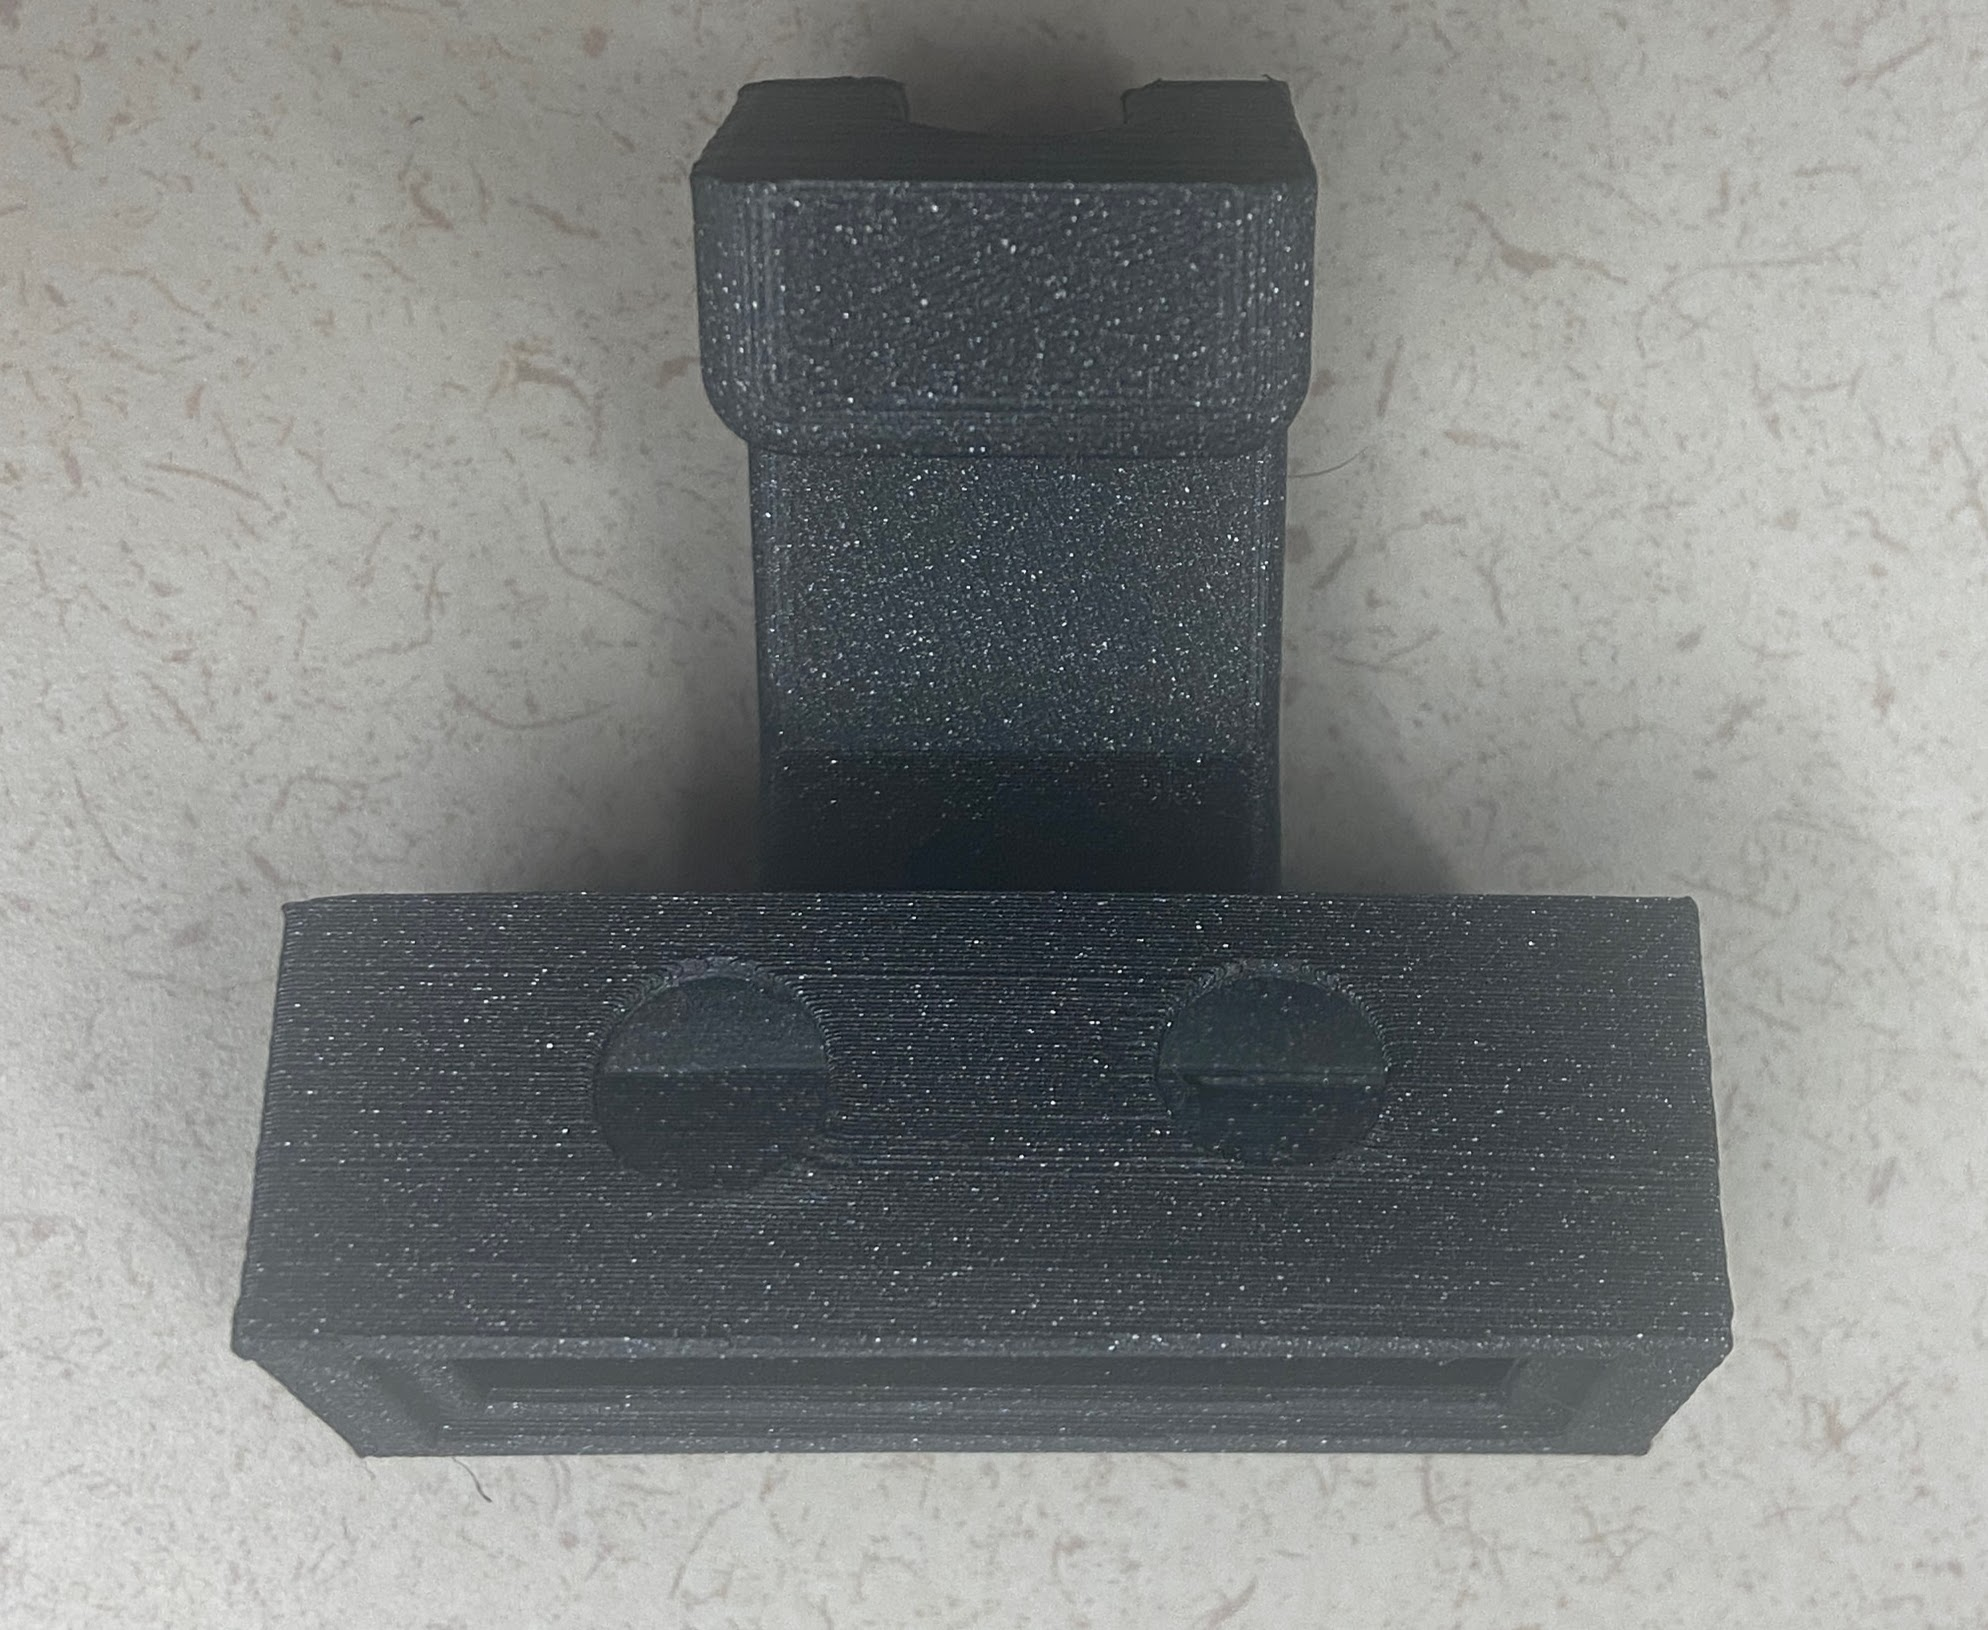
\includegraphics[scale=0.1]{diagrams/builtUnits/buttonhousingEmpty.JPG}
        \caption{3D-printed thumb rest with housing for buttons below.}
        \label{fig:buttonThumbrest}
    \end{figure}
\end{center}

These attachments are optional and not needed for the Cyberinet main unit to be functional and are intended to only be connected when needed for a particular performance. All the expansions connect utilizing a standard USB-C connector. However, these units do not utilize the USB protocol, so both the main unit and expansions cannot be connected to a computer via these ports. Because the Cyberinet does not communicate to these using USB protocol, not all USB-C cables can be used for this, however the vast majority can. While a set of USB-C cables that are functional is included with the full Cyberinet set of hardware, The main reason for utilizing this connector is for the end-user to be able to supply their own cables of various lengths depending on their needs. 


\begin{center}
    \begin{figure}
        \centering
        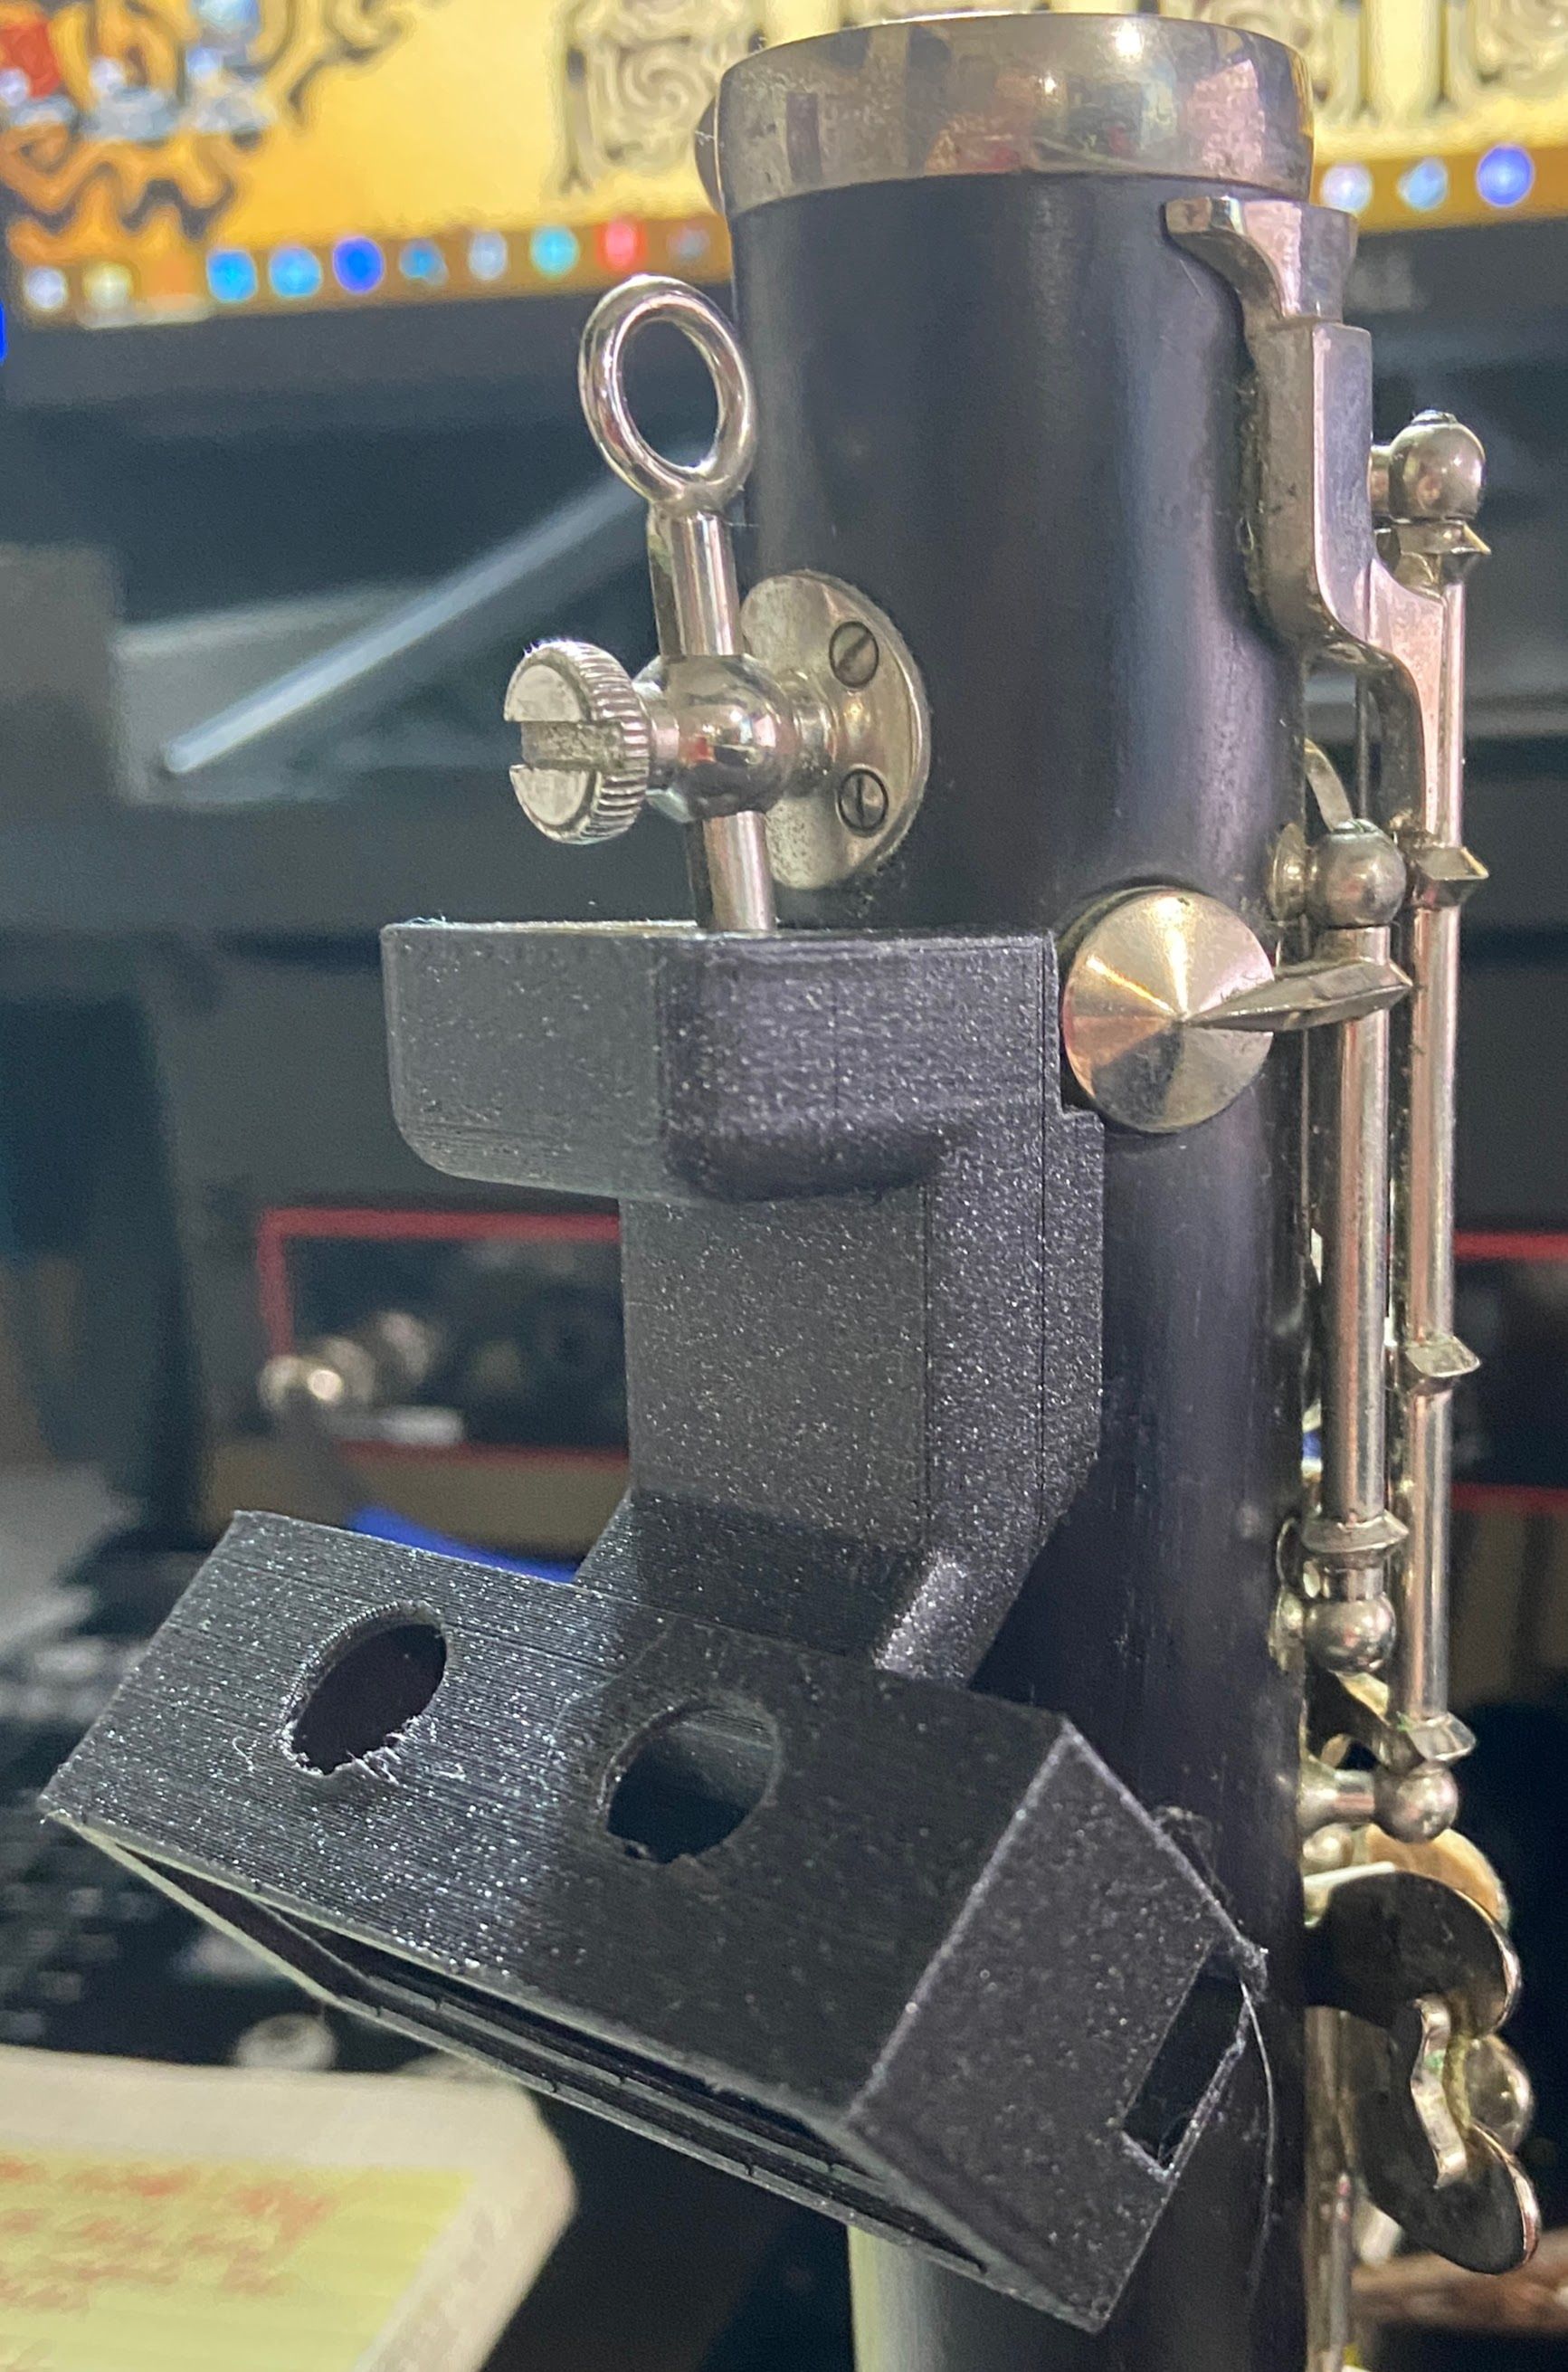
\includegraphics[scale=0.08]{diagrams/builtUnits/thumbOnInst.JPG}
        \caption{Empty Button Expansion placed on a Clarinet thumb rest}
        \label{fig:thumbOnCase}
    \end{figure}
\end{center}

This board, while optional, is incredibly useful for a performer on stage. They can access the buttons using their right thumb when performing. This maneuver is easier when utilizing a neck strap, so the performer can place the buttons elsewhere if they like using a longer connector cable. The closeness between the buttons and thumb rest is shown in figures \ref{fig:buttonThumbrest} and \ref{fig:thumbOnCase}. Each button also contains a single, colored LED built into it to provide feedback to the performer. By default, the lights are only illuminated when the button is pressed. The Cyberinet simply detects whether a button has been pressed and transmits that data as a Boolean value to the computer. Using a program such as Max, the user can have the buttons achieve functions from near limitless hypothetical list of options. For this project, the buttons were used to trigger microphone recording and buffer playback, however objects that take the button input and move between various presets, trigger DSP, and turn pages of a score have also been developed and included in the software bundle for this project.

\subsubsection{Other Expansions}
At the time of writing, only a single other expansion unit has been completed. This is the Volume Detection unit which contains an Adafuit I2S MEMS Microphone Breakout board. Like the Button Expansion, this unit is housed in a 3D printed case and connects to the Main unit with a USB-C cable. 

This unit is designed to respond to the volume of the local area, and is designed to be placed in a variety of different areas. By placing the sensor at different distances from the performer or speakers, the sensor can more or less sensitively respond to the volume. The user is only limited by the length of USB-C cable they can utilize. The Cyberinet detects when the volume at the sensor exceeds 0 dB, and transmits the data as a Boolean value to the computer in a similar manner to the Button Expansion.

\section{Physical Design}
In order to minimize the total number of parts required for the Cyberinet, the electronics are housed in a newly designed plastic unit. This Main Unit is intended to replace the barrel and mouthpiece of the original instrument when in use. In addition to the main unit, the Button Expansion as well as any future expansions have a 3D printed body in order to control the expansion's ergonomics and protect the electronics.

\begin{center}
    \begin{figure}
        \centering
        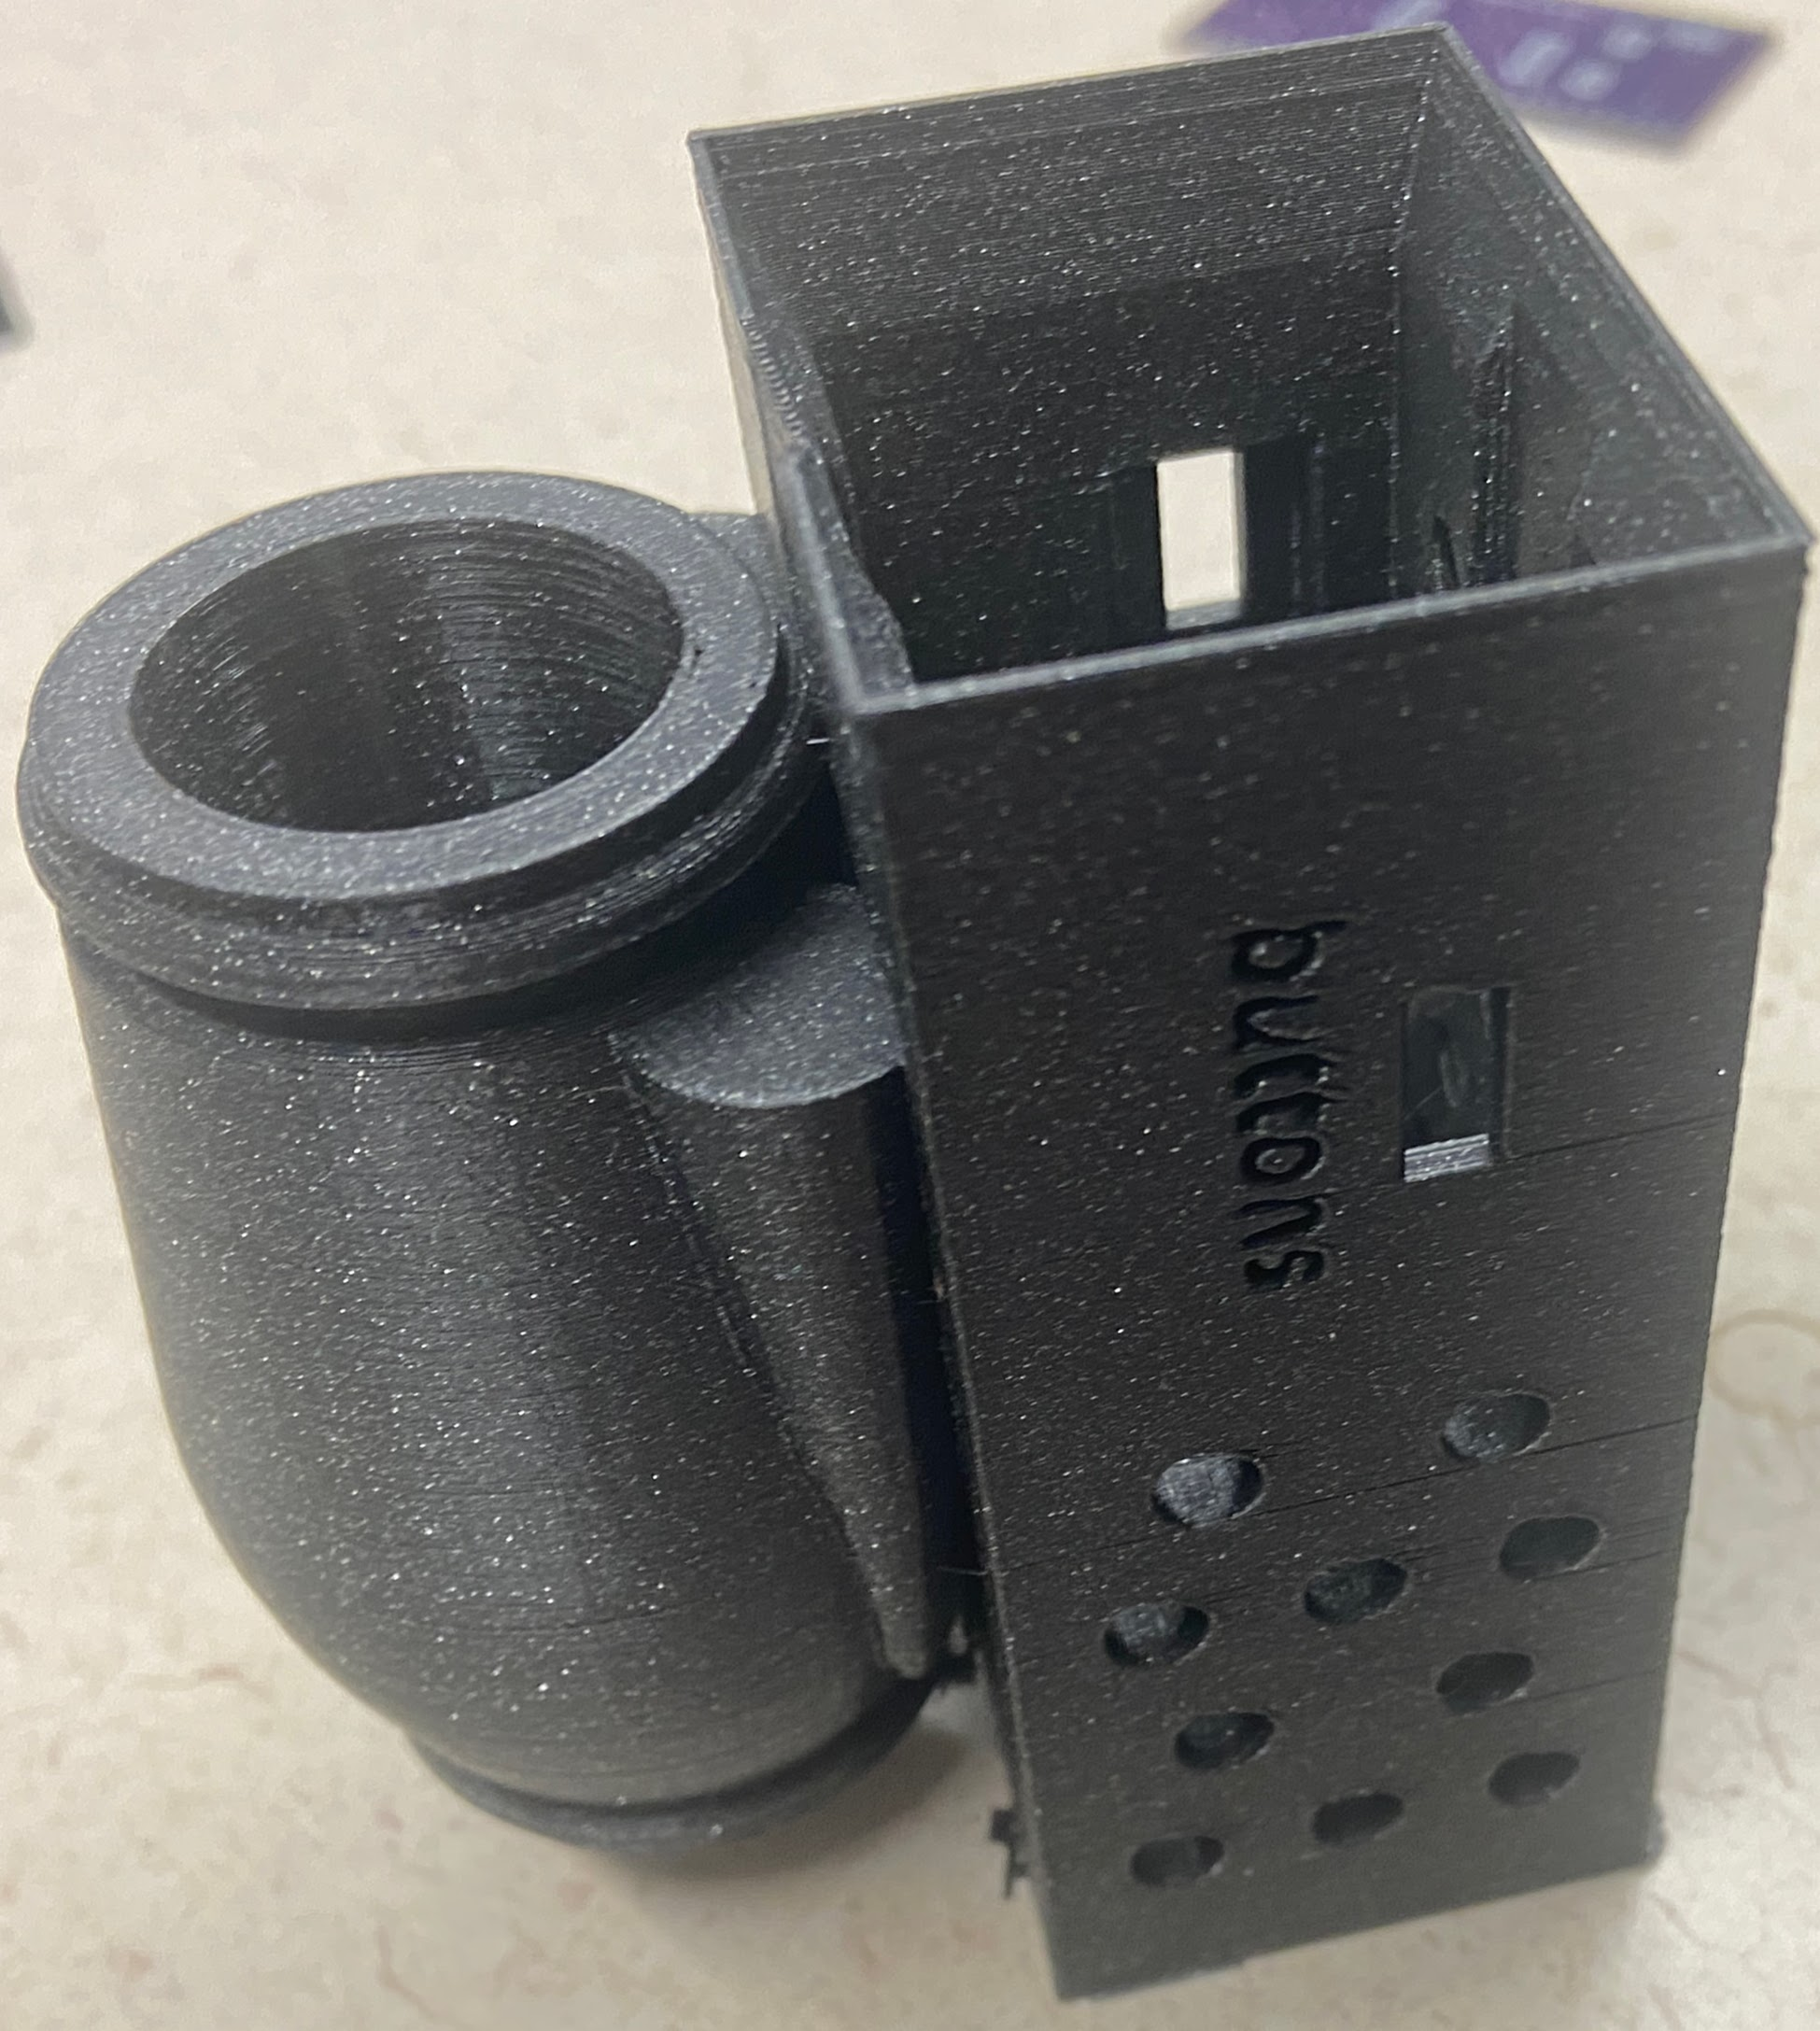
\includegraphics[scale=0.1]{diagrams/builtUnits/emptyCase.JPG}
        \caption{Empty 3D Printed Cyberinet Housing}
        \label{fig:cybernetCase}
    \end{figure}
\end{center}

All materials are printed using either PLA or PetG material during prototyping. These materials were chosen for their relative low cost, ease of production, and density. For the final version, PLA was utilized because the sound quality of the material most closely resembled that of the original clarinet. All parts were printed on an Original Prusa i3 MK3S+. Because of the testing of different materials, several images in this document may be in largely varying colors. The final version was printed to be black or dark grey, however future revisions could see an option for custom colors when printing. 

While it is intended to remove the Clarinet's uppermost parts and replace them with the Cyberinet when needed, it is possible to perform using the hardware while powered off for a traditionally acoustic performance. The usage of this feature is at the discretion of the performer.

\section{Main Unit Assembly}

The main unit of the Cyberinet is designed to replace the uppermost portions of a B-flat clarinet: The barrel and mouthpiece. As shown in figure \ref{fig:cybernetCase}, the electronic components are housed in the box on the side of the instrument. Placing the electronics here allows for the unit to be easily adjusted for tuning or be easily removed as needed. The box was made as small as possible, but it still contains all of the electronic components, excluding those in any external add-on components. 

The electronics were housed in the upper portion of the clarinet for two main reasons. The more minimal of the reasons is that the differential airflow pressure is much greater in the clarinet before the air can escape through the key holes. By locating the sensor here a wider range of values are possible than if it was located lower on the clarinet's tube. However, this could be remedied with additional tubing if the location of a unit needed to be otherwise located. Speculating on this is outside of the scope of this document however.

The second and more necessary reason for the placement of the Main Unit in the upper portion of the clarinet is weight. While not overly heavy at GIVE THE WEIGHT OF THE FINAL UNIT HERE one may not think it would cause difficulties in performance. But when thinking of the clarinetist as a Second Class lever, insight can be gained on the specifics of this issue. % don't need to break down into levels nd physics for this

To assemble a Cyberinet main unit, first the case must be 3D printed. Because of the process of 3D printing and the necessary thickness of the material needed to preserve sound quality, the printing process takes approximately 12 hours to complete. Because of this, it is recommended to begin printing the units first, then work while the case is being completed by the printer.

All components are connected utilizing a custom printed circuit board. This is done to help connect all of the various pins for data collection and power distribution in as small of a space as possible. The PCB is shown in figure \ref{fig:mainUnitPCB}.

\begin{center}
    \begin{figure}
        \centering
        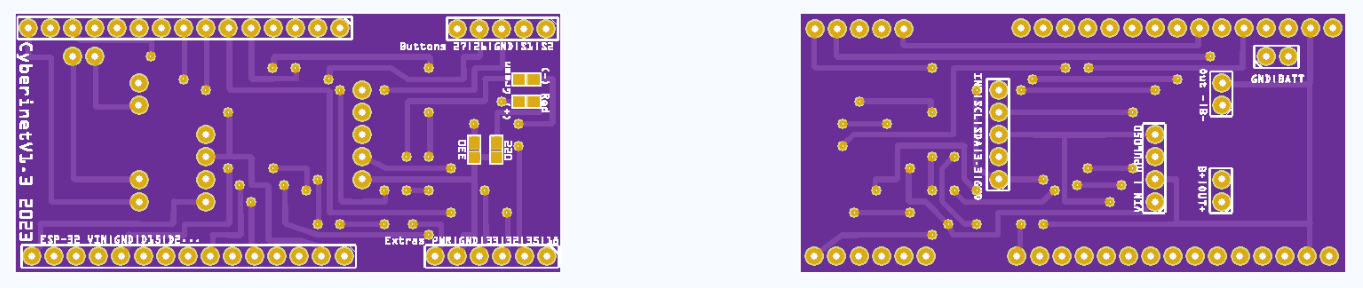
\includegraphics[scale=0.6]{diagrams/PCBs/cyberinetPCB.png}
        \caption{Cyberinet Version 1.3  Main Unit PCB Diagram}
        \label{fig:mainUnitPCB}
    \end{figure}
\end{center}

As shown in the following breakdown, assembling the Cyberinet must be done by working with the smallest components and working up to the larger ones. This is because several components are placed over other ones and it becomes exponentially harder to assemble a Cyberinet should one have to begin working around the placement of a sensor or remove a chip to adjust or repeat a step\footnote{It is recommended to pause and check the connections after soldering each component for this reason as well}.

First, the Surface-Mounted components are soldered onto the main board. These include the 2 on-board LEDs and their accompanying resistors. Following this, ribbon cables and the USB-C and JST connectors are then soldered into place on the PCB. The third step is to solder the power distribution (TP-4056), gyroscope (MPU-6050) and airflow pressure (SDP-31) chips into place. The white silkscreen rectangles show which side of the PCB each component belongs on, and the text indicates which orientation is needed for each component to help ensure a correct alignment.

The airflow pressure sensor (SPD-31) is lifted away from the PCB with the use of a pin header. This is done to avoid any accidental shorts between the contacts on the two boards. While not required, this can be done to the gyroscope (MPU-6050) as well. The final soldering step is to connect the ESP-32. Because of its size, this chip is kept opposite from the sensors and is also lifted using pin headers for the same reason as the SDP-31.

\begin{center}
    \begin{figure}
        \centering
        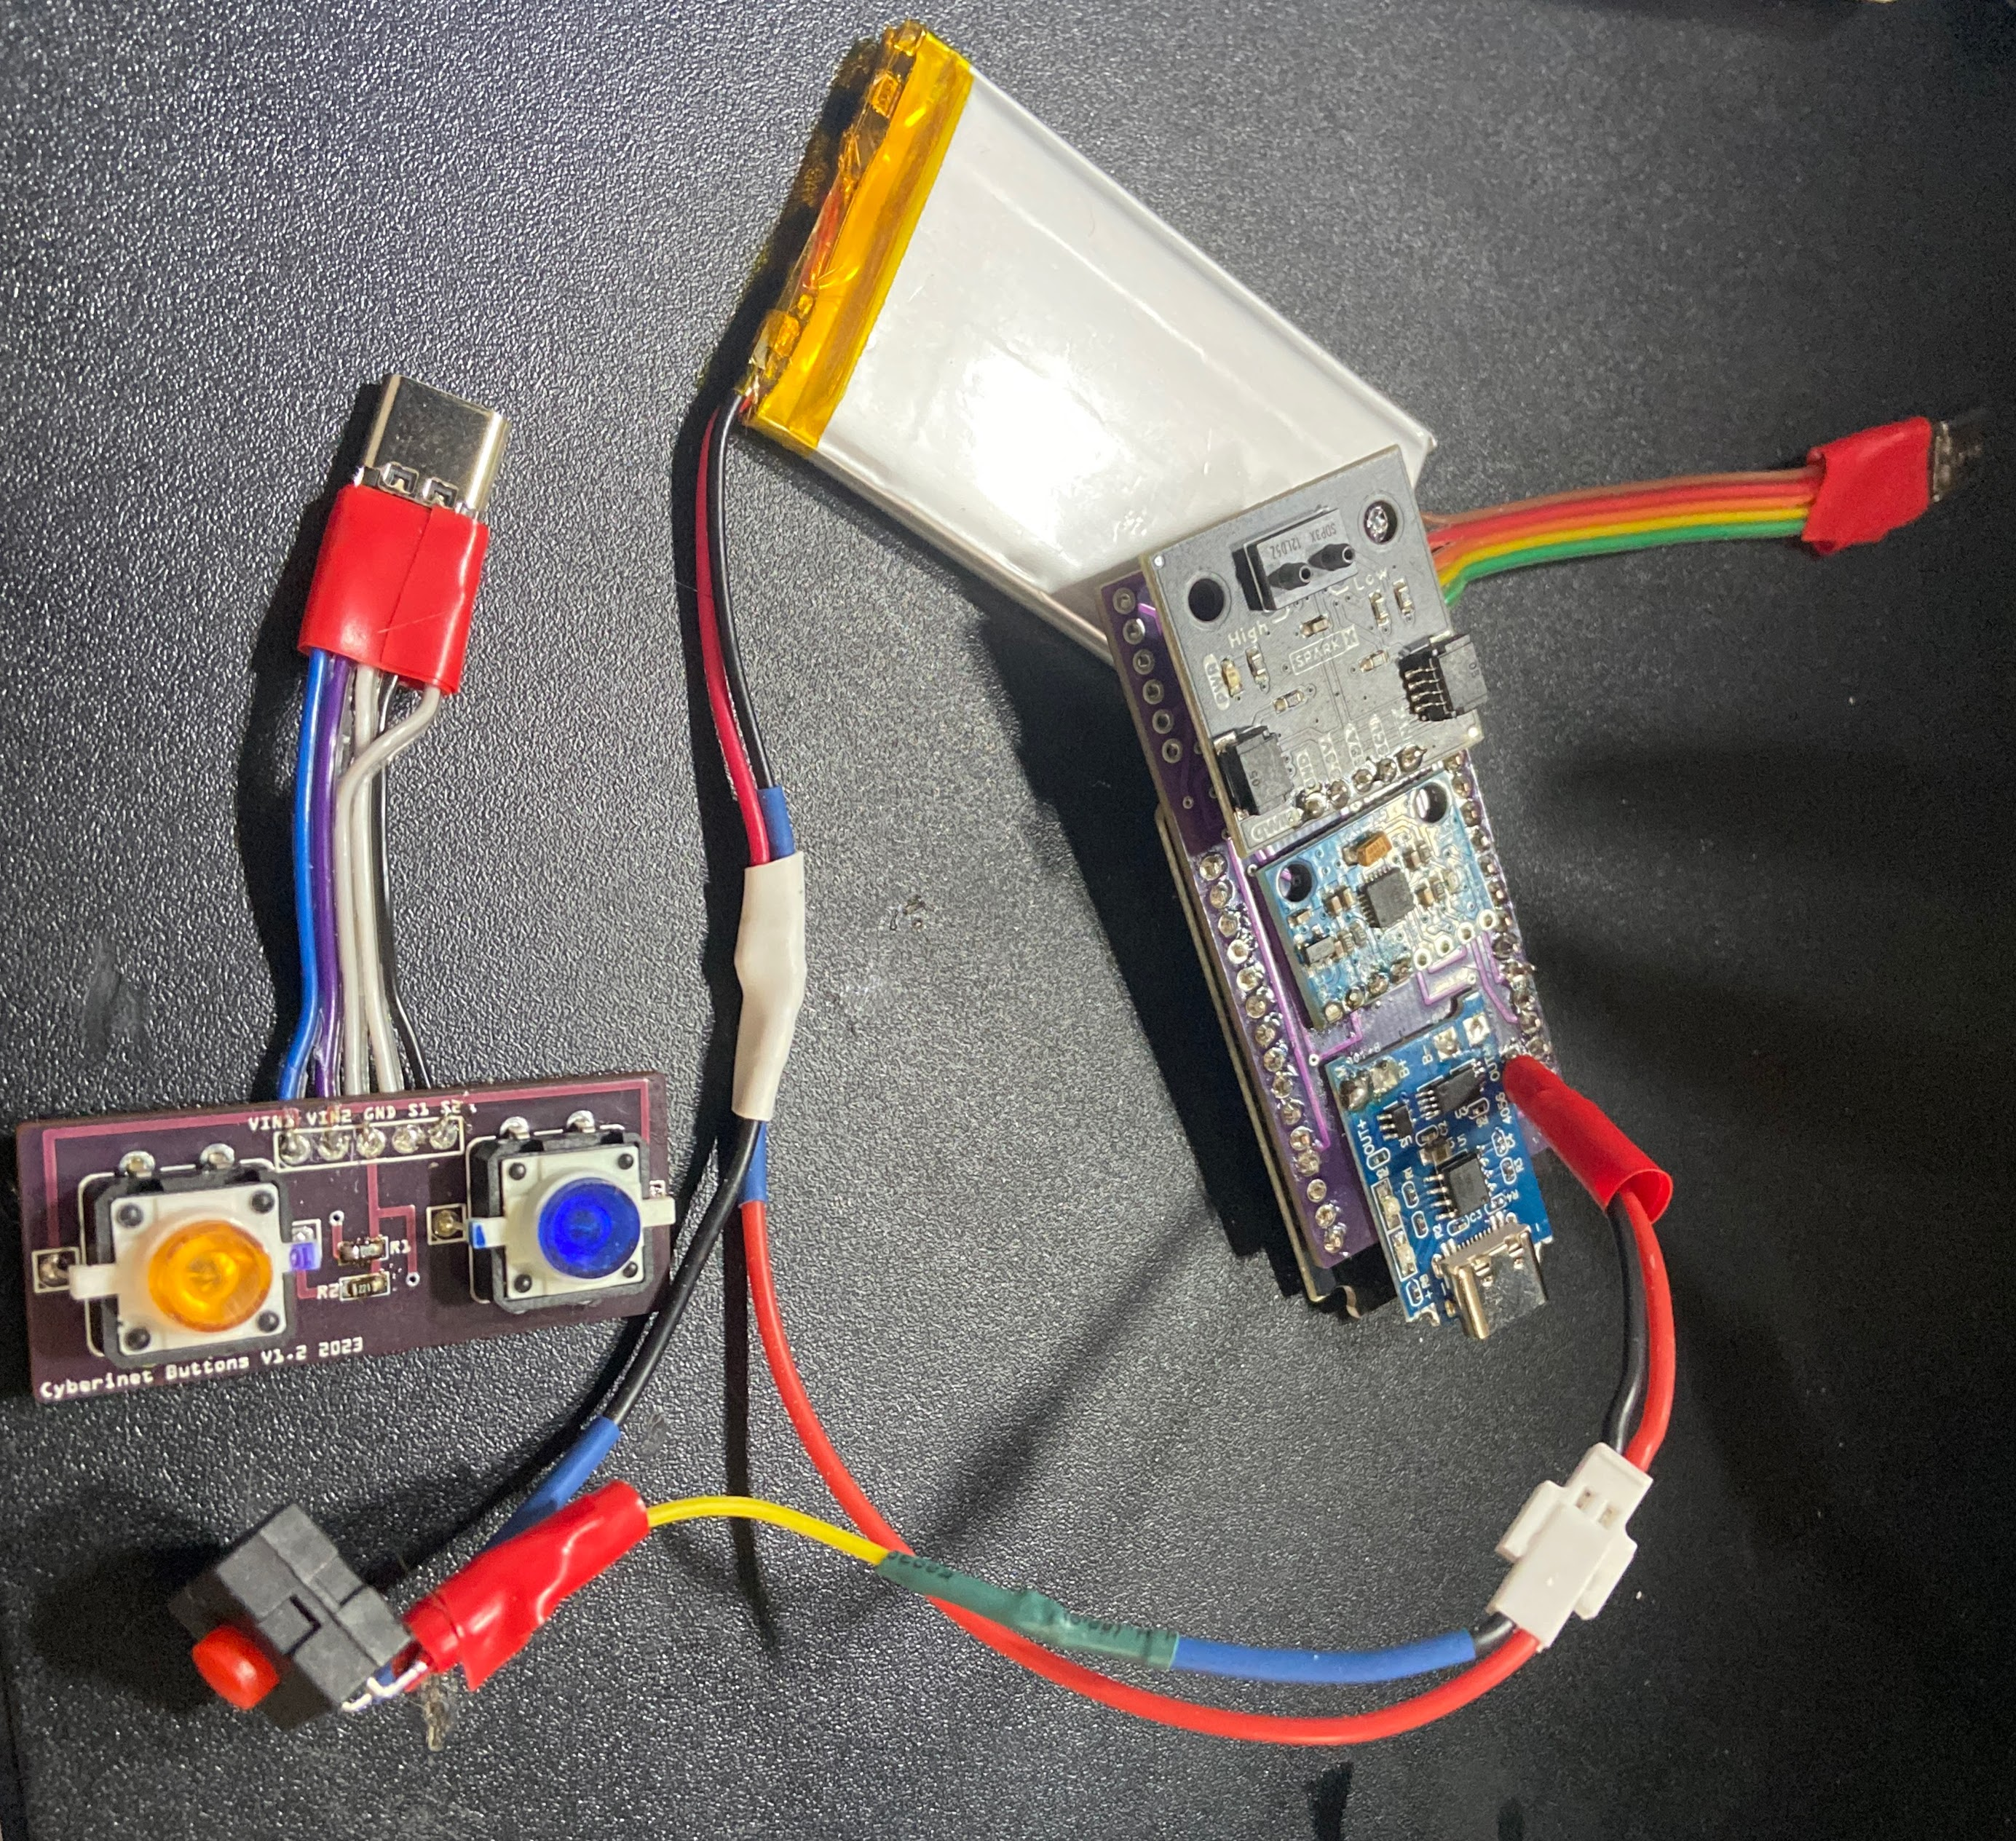
\includegraphics[scale=0.1]{diagrams/builtUnits/noCase.JPG}
        \caption{Completed Cyberinet and Button Expansion without 3D printed housings}
        \label{fig:CyberinetNoCase}
    \end{figure}
\end{center}

When complete, the whole unit is slid into the 3D-printed case. Ports and tubes are aligned to the appropriate places and glued down to avoid unwanted movement. Not taking into account the space needed for the battery, tubing, and wired, the final Main PCB is approximately 5mm deep, creating a compact unit that can be easily placed in a variety of locations.

\begin{center}
    \begin{figure}
        \centering
        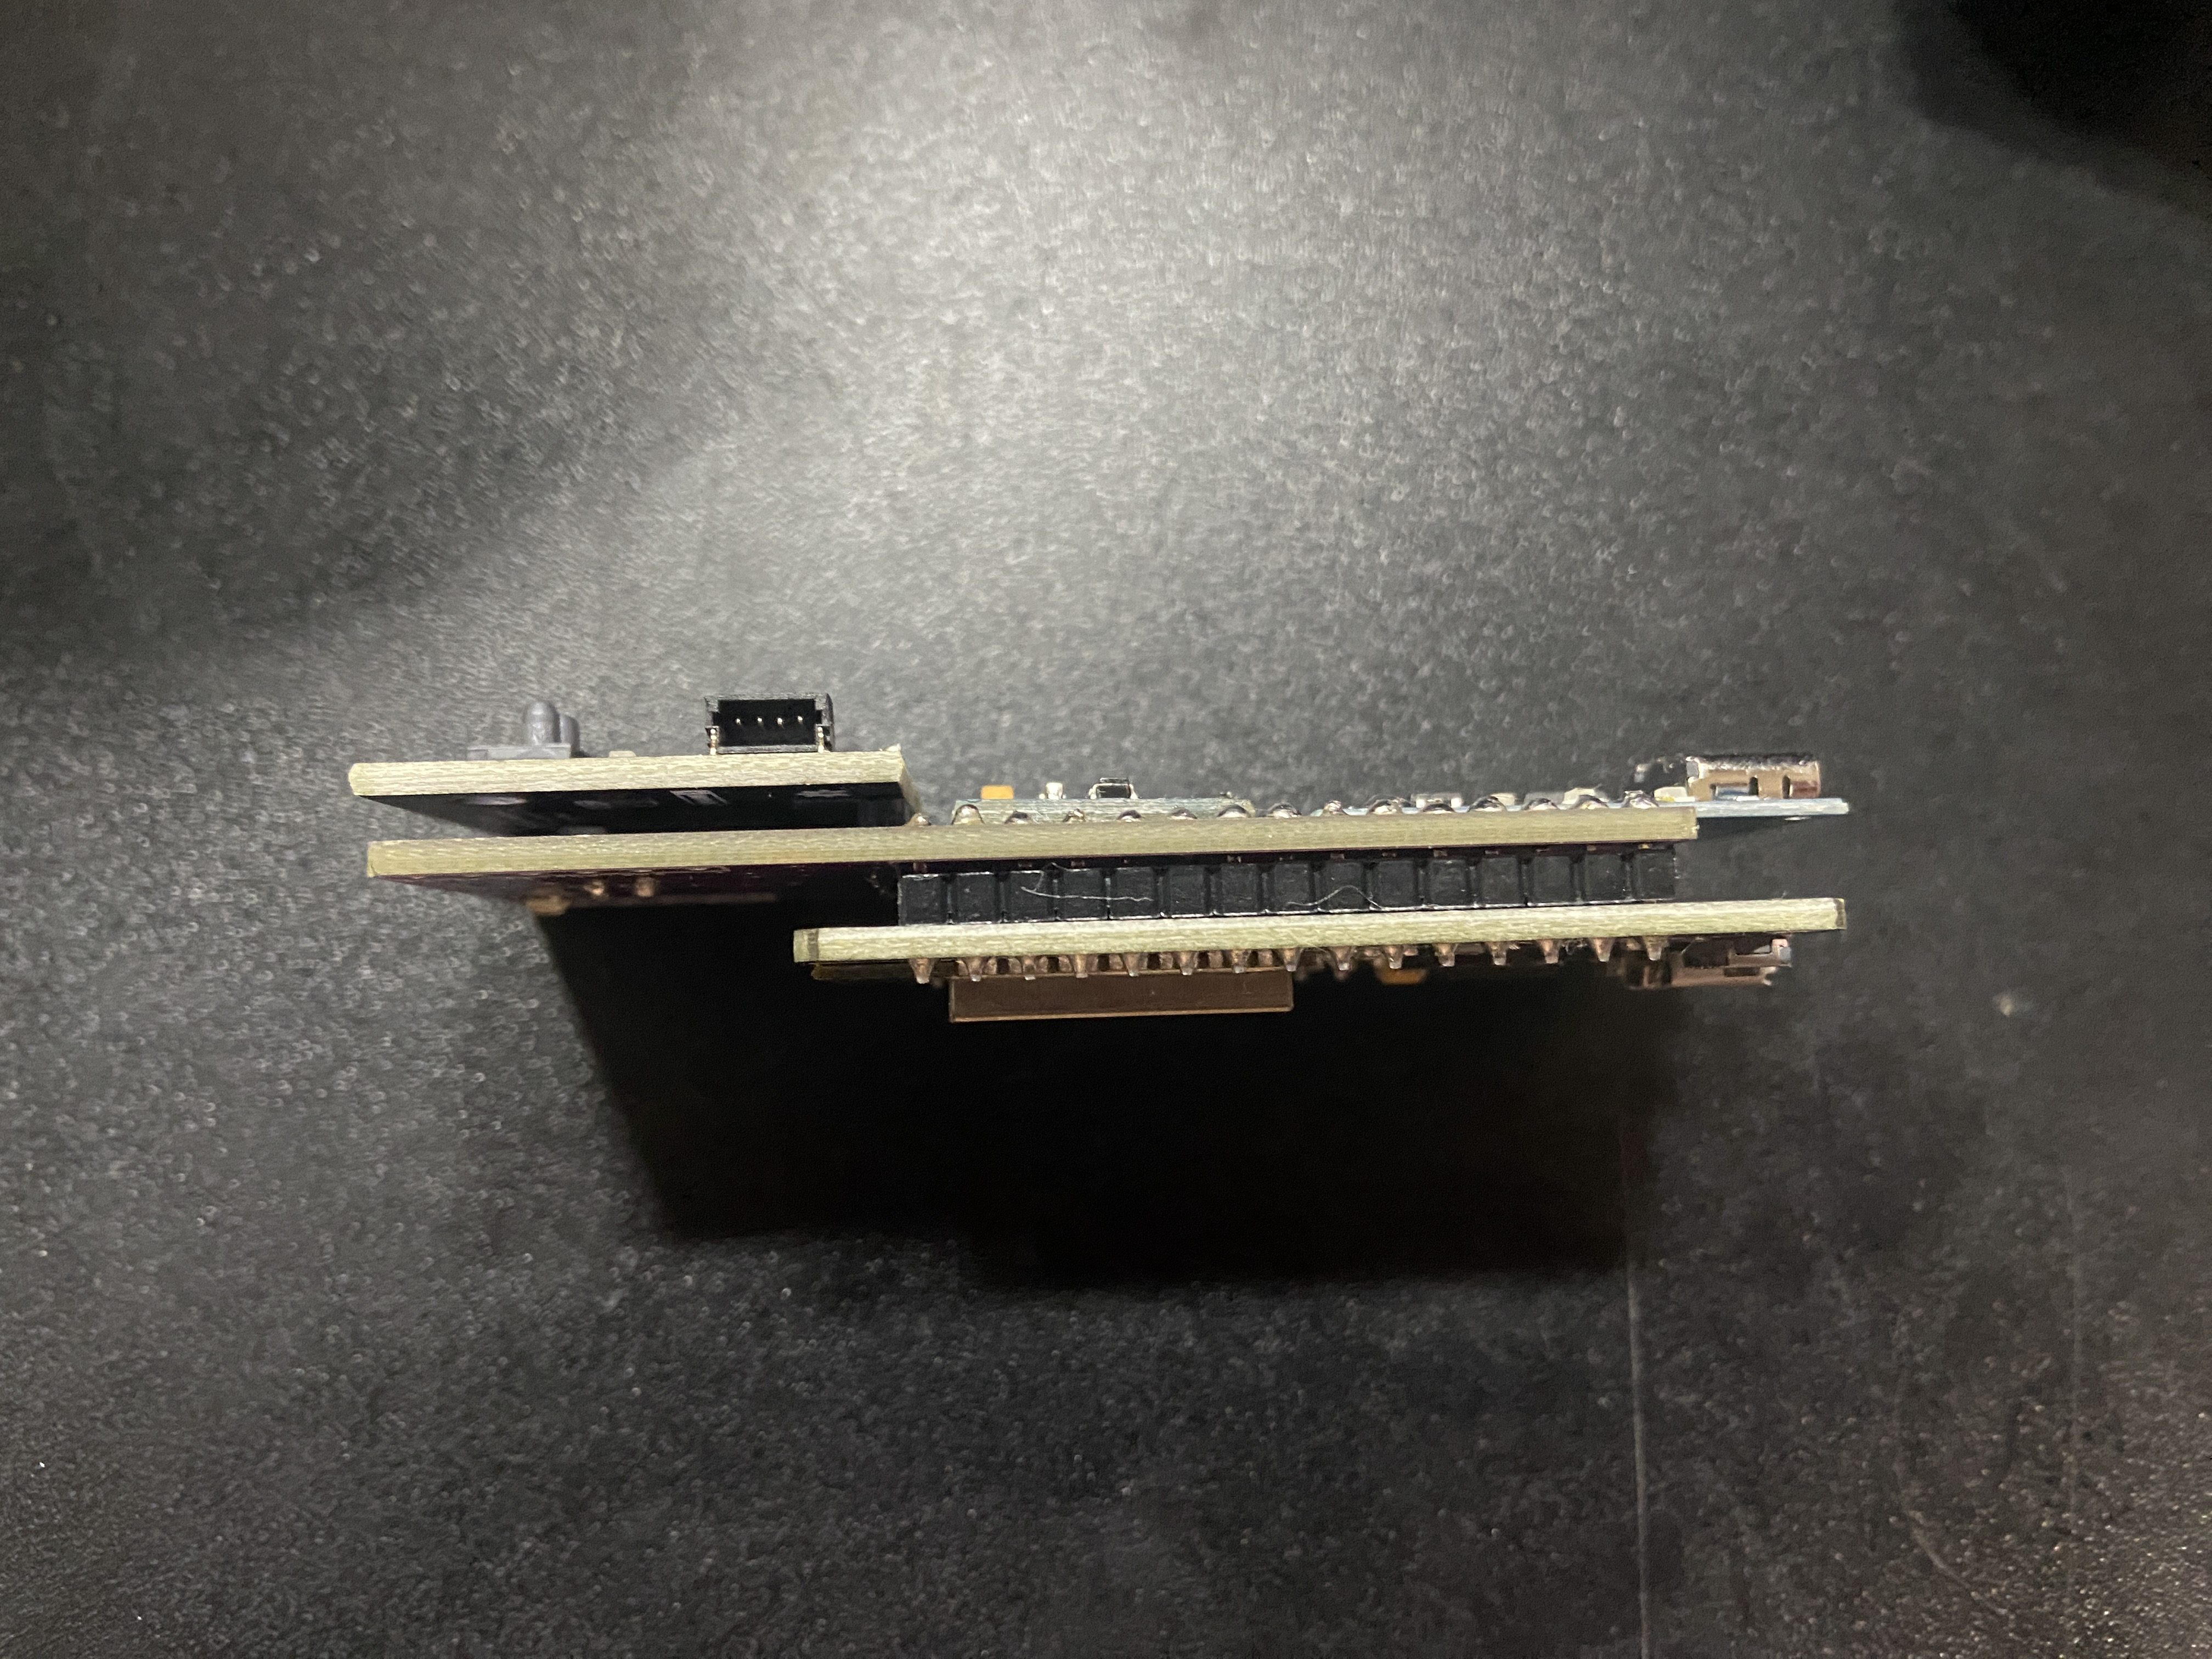
\includegraphics[scale=0.05]{diagrams/PCBs/cyberinetThin.JPG}
        \caption{Cyberinet Sensors Side View (No Casing or cables)}
        \label{fig:Cyberinetside}
    \end{figure}
\end{center}


Overall, placing the Main Unit's bulkiest components as close to the performer's mouth as possible results in the least amount of extra effort required to perform with the instrument. It is impossible to completely remove the added weight of the system additional, but this placement minimizes its impact on the performer.


\subsection{Expansion Assembly}

The Button Expansion is much simpler when compared to the main unit. The unit is composed of only two mechanical buttons with built in LED's, two resistors for those LED's, a USB-C port for communication with the Main Unit, a PCB to route all of the connections and the 3D printed housing. The button expansion is designed to be attached to the performer's thumb rest to allow for easy access with the right thumb. However it is also shaped in a way to allow for it to be held in the hand or placed elsewhere.

In the current software version, the button LED's are only illuminated when the buttons are pressed. However they are wired independently of the switches on the expansion. In future versions, the ability to control these LED's via the software is planned.

To assemble the unit, all components are soldered to the PCB. Like the Main Unit, SMD components are attached first, followed by cables, and finally the larger components. The completed PCB is then secured within the 3D-printed housing to complete the unit. The PCB for the Button Expansion is shown in figure \ref{fig:buttonPCB}, and the version containing all of the components soldered to it is part of figure \ref{fig:CyberinetNoCase}.


\begin{center}
    \begin{figure}
        \centering
        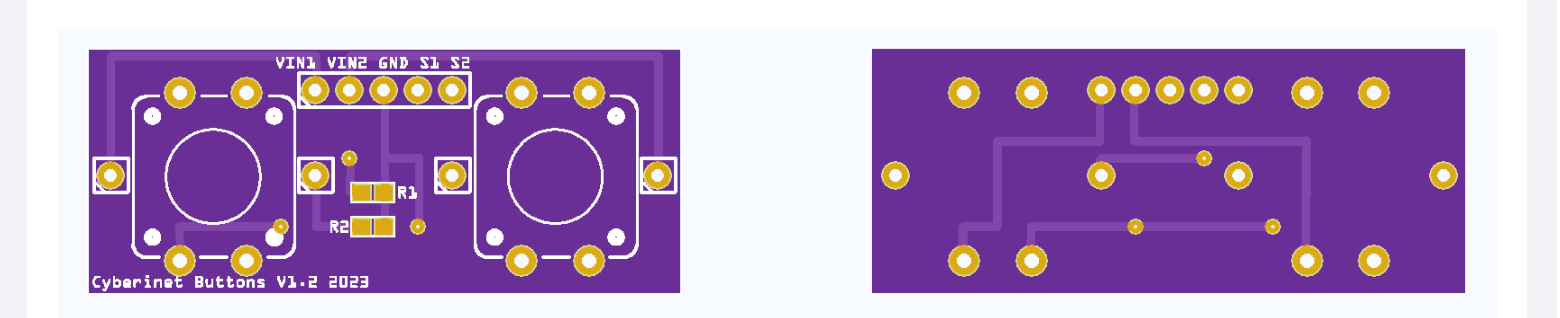
\includegraphics[scale=0.5]{diagrams/PCBs/buttons1.2.png}
        \caption{Button Expansion PCB}
        \label{fig:buttonPCB}
    \end{figure}
\end{center}


\section{Future Hardware Directions}
At the time of writing, the Cyberinet is only available for B-flat soprano clarinets. While this is the most commonly found Clarinet, it represents only a fraction of the total woodwind family. In the future, plans to adapt the hardware case to fit different instruments will allow for the Cyberinet to be utilized in an exponentially larger number of scenarios. 

First, adapting the unit for the A Clarinet and Bass Clarinets. At this time there are no plans to expand to an E-flat Clarinet due to the limited space to attach electronic components. Following the Clarinet expansions, ideas for compatibility with Saxophones and Flutes are being discussed, but require more planning in order to make functional units.

Outside of the aforementioned hardware needed to make the Cyberinet framework compatible with more instruments, an increase in modular expansions is also planned. Initially only additional buttons and a volume-sensing microphone are available, but plans for the following sensors to be released in the future have been made:

\begin{itemize}
    \item Pressure Sensor: responds to varying pressure on the instrument's keys. Needs special mounting of Force-Sensitive-Resistors, as well as doughnut-shaped FSRs.
    \item Pitch Detection: Works like the tuner software object. This will display tuning information and transmit pitch information to the computer. Needs hardware with adequate Analog-to-Digital Conversion.
\end{itemize}


\chapter{Programming the Cyberinet}
This chapter discusses the code located within the Cyberinet itself, as well as the accompanying library of Max tools. Discussion of the software portion of each of the included music compositions will be discussed in that chapter. In short, the Arduino code and the Max objects work together in order to achieve the four main steps in the functionality loop of the Cyberinet:

\begin{itemize}
    \item Step 1: Collect Data
    \item Step 2: Transmit Data
    \item Step 3: Receive Date
    \item Step 4: Route Data
\end{itemize}

\section{Arduino Code}
Another positive feature of the ESP-32 is that it is able to be programmed utilizing a variety of languages and environments. For the Cyberinet, the micro-controller was programmed using the Arduino coding language and Arduino IDE version 1.8\footnote{Arduino IDE Versions 2.0 and 2.1 were released during the Cyberinet's development, but were not utilized to avoid any compatibility issues during development. Future software versions will be created in more up-to-date IDEs.} This section will break down and discuss the components of the Cyberinet's on-board programming. The full .ino file's text can be found in this document's appendices.

\subsection{Collecting Data}
In order to collect the data from the sensors, each sensor has been given a function within the Arduino code. These functions serve the main focus of collecting and transmitting data. However because of the differing OEM sensors, each one utilizes a slightly different method of data collection and has a different range of values that can be expected. These functions are called in every loop of the program. Figure \ref{fig:getButtonsGetAir} shows the two most straightforward of these functions in their entirety.

\begin{center}
    \begin{figure}
        \centering
        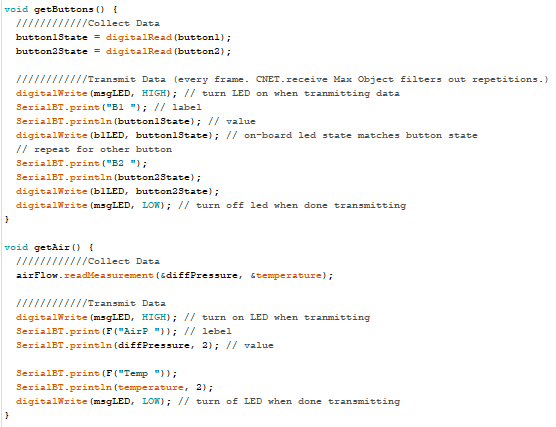
\includegraphics[scale=1.5]{diagrams/maxPatches/getbuttonsgetair.png}
        \caption{Cyberinet getButtons() \& getAir() functions.}
        \label{fig:getButtonsGetAir}
    \end{figure}
\end{center}

Looking at the function getButtons(), we can see the simplest of these functions. This function looks at pins 12 and 14 on the ESP-32, which are connected to the Button Expansion's USB-C connector. By utilizing the ESP-32's built-in pull-up resistors, the Button Expansion returns a 1 when the button is not being pressed and a 0 when the button has been detected as being clicked.

getAir() works in a similar function to getButtons(), but with a slightly different code because of the SDP-31's I2C connection and coding library. Because of this, the ESP-32 contacts the SDP-31 on its I2c address and requests the specific data at 2 registers. These data are labelled as 'diffPressure' and 'Temperature' respectively. 

The function 'get5060()' is shown in figure \ref{fig:get6050}, and contains a few more complicated steps than the previous functions. This function begins by communicating with the MPU-6050; essentially waking it up. Next, the data points for the gyroscope and accelerometer are requested. It is at this point that the function begins to differ from the previously mentioned ones.

\begin{center}
    \begin{figure}
        \centering
        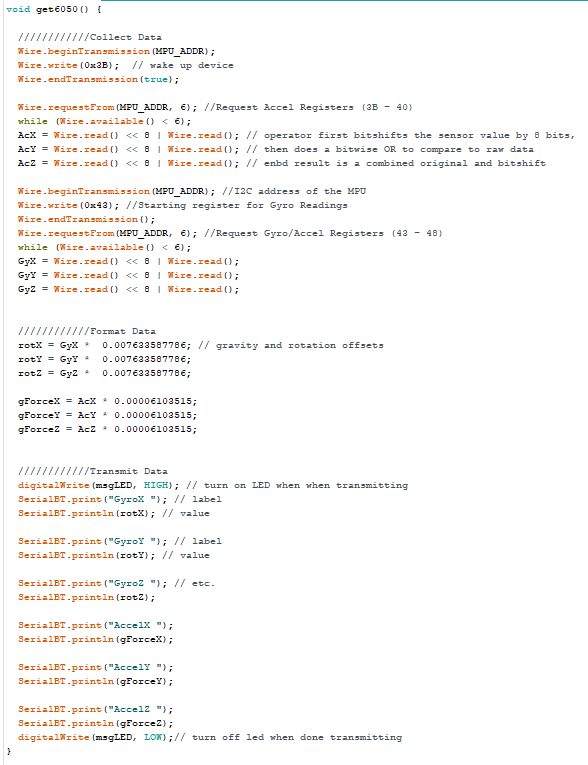
\includegraphics{diagrams/maxPatches/get6050.png}
        \caption[scale=1.5]{Cyberinet get6050() function.}
        \label{fig:get6050}
    \end{figure}
\end{center}

All six of the requested data points are then shifted over by 8 bits and then added to a second reading of the remaining data. This is done in order to fully read all 16 bits of data from the MPU-6050 on devices unable to access and process all 16 bits of data at once. 


\subsection{Transmitting Data}
The final portion of the data collection functions is the transmission of the data. This is done using the bluetoothSerial library, which allows for the ESP-32 to utilize serial communications over a Bluetooth connection. The .ino code's setup function is responsible for setting up these connections. The port is titled "CyberinetV13", indicating the version number with no spaces or punctuation, and utilizes a baud rate of 115200. This library contains the main Serial functionality present in Arduino, and simply is called with the instance name SerialBT to indicate the transmission is a wireless one.

Once all of the data is collected it is transmitted using the SerialBT.print() and SerialBT.println() commands. Utilizing the Max formatting, a label is created for each data point being transferred, then the individual value is transmitted, separated from the label with a space and ending with a carriage return. Each of the labels are as follows:

\begin{itemize}
    \item GyroX
    \item GyroY
    \item GyroZ
    \item AccelX
    \item AccelY
    \item AccelX
    \item AirP
    \item Temp
    \item B1
    \item B2
    \item Exp
\end{itemize}

The data is sent in serial data packets, and the spaces and carriage returns are utilized by Max to help isolate the individual data and label values. The raw data stream as it appears in the Max console is shown below. To indicate that a data transmission has occurred, the red message LED is illuminated immediately before and toggled off immediately following the completion of the transmission. The end result is a rapid blinking of the red light when the Cyberinet is functioning properly. When combined with the green power indicator LED, the result can be perceived as a light changing between green and yellow through the holes in the 3D printed case.

% screenshot of the max console with all the values

The measured latency of the data transmission is measured at approximately % finish testing 

That value was repeatedly testing with the CNET.latency patch, which is discussed more in section 4.2.2. In order to arrive at the averages shown in figure % need to make figure with values after testing.
the test was repeated 10 times at 3 different distances from the control computer. 2 meters, 5 meters, and 10 meters were selected to represent a close, medium, and far distance while still remaining in the normal Bluetooth range\footnote{The current version of Bluetooth has a range of approximately 10 meters}.

CNET.latency can be utilized by anyone who needs to test the latency of their hardware unit. When loading the patch, and connecting the Cyberinet, a microphone and the button expansion are also needed. The user will place the microphone close to the buttons and press one of them which makes an audible click. This audible click is recorded, and then used to gate a small burst of white noise, which then is output from the speakers and picked up by the original microphone. Max then compares the number of milliseconds between the first button click and the burst of white noise from the speakers. This comparison calculates the full latency from an action on the Cyberinet to its result being herd by the user. The results of these tests are shown in figure  

\section{Max Programming}

To utilize the data being collected by the Cyberinet’s hardware, I have created a small library of Max objects to help with the collection and usage of said data. While detailed below, it is important to mention that Max is a paid software. The software and hardware components are all open source, however in order to create your own patches, the end-user will need to download the software. If saving patches is desired, then they must purchase a software license. Potential freeware options are being considered and will be explored upon more in a later chapter, but at the time of writing, are not in active development.

\subsection{Receiving \& Routing Data}

Once the serial data has been transmitted from the Cyberinet, it moves into the connected computer. This connection utilizes Bluetooth, and can be easily managed in the Max software\footnote{Max version 8.5 or newer is needed when working with the Cyberinet}. A single object is utilize in order to help receive and parse the data stream from the Cyberinet. CNET.receive allows the user to easily determine which Bluetooth port to receive data from, then sends it to various object outputs for use in the Max environment.

% picture of inner workings of CNET.receive
% \begin{center}
%     \begin{figure}
%         \centering
%         \includegraphics{}
%         \caption{Caption}
%         \label{fig:my_label}
%     \end{figure}
% \end{center}

In short, this Max object runs a small Node script that helps to import the data into Max. This script specifies the desired serial port, then using the space and carriage return characters, formats the data into the label and value pairs that Max expects. These values are then routed to individual outlets based on their labels\footnote{Each outlet is given a label so that the user can identify what the numbers leaving the object are}. Prior to leaving the outlets, the data is then scaled to fit a range of 0-1. This helps to keep all of the sensors within an easily adjustable range for other objects within Max. The only exceptions to this are the buttons which only output 0 or 1 when the button state changes, and the temperature which is measured in degrees Celsius and not scaled at all. 

In order to utilize this object, you must first connect the Cyberinet to the computer via Bluetooth. after the connection has been established, sending a bang into the first inlet will open communications on the default port. If the desired port is not the default, then sending the message "setPort" followed by the port name will change this. From there data will begin automatically flowing through the patch to the desired outputs. If you wish to see the raw, un-scaled data in the Max console, toggle the second inlet on. A bang to inlet three will stop communications, and a bang to inlet four will install appropriate NODE drivers and dependencies to allow Max to utilize the javascript code. This is only required one time on each computer.

\subsection{CNET Objects}

While not necessary for the functionality of the Cyberinet, I have also created a small collection of Max objects for use with the unit. These objects were all used within the Compositions discussed in chapter 6. All of these objects are designed from the ground up to receive data from the Cyberinet in order to control their functionality. These include:

\begin{itemize}
    \item reverb~: a Schroder style reverb based on examples from CCRMA.
    \item compressor~: Based on the compressor objects created by Cycling74.
    \item delay~: A single delay line using the tapin~ and tapout~ objects. 
    \item MultiDel~: A delay line utilizing 4 different tapout~ objects to create multiple delay lines. Each one can have its individual output level set for unique mixing capabilities.
    \item feedbackDelay!: Identical to the simple delay, but with a feedback option added.
    \item vibDelay!: Functions similar to the Simple delay object, but includes a basic implementation of FM synthesis to adjust the pitch of the signal to be delayed. 
    \item tuner: This object functions like most other tuners available on the market. It will determine the pitch of an incoming signal and output the value as a signal. This is useful for checking and maintaining tuning within the Max environment, and for having the Max patch respond to certain pitches. This object requires a microphone be used to monitor the input as the ADC capabilities of the ESP-32 DEVKIT are unable to pull off this effect.
    \item pitchShift~: changes the pitch of an incoming signal. This can be controlled by MIDI  numbers or the 0-1 floating point range of the Cyberinet. The values input here are the desired pitch of the signal, not the amount by which it is shifted. both his and CNET.tuner also have a dry digital pass-through and latency monitor,
    \item latency: Designed to test the latency of the Cyberinet within  the Max environment.
\end{itemize}

In addition to the above objects, the Cyberinet software also includes a few objects intended to be helpful in setting up and trouble shooting. The main one of these objects is the tuner object. This object serves as a tuner within the Max environment, allowing for quick adjustments to be made without needing an additional piece of hardware. 
The main downside to the tuner object is that it requires the use of a microphone input to the computer. This is due to the limited ADC capabilities on the Cyberinet's main ESP-32 Board. However, an unexpected upside to the object is it's pitch detection capabilities. The tuner object is able to detect both the musical pitch of the incoming signal, but also fine tuning in cents. Because this information is expressed in MIDI, it can be used to trigger a variety of other events in the max environment. While the list of possibilities is extensive, the idea of having the max patch harmonize with the clarinet is one of particular interest to the author.

\subsubsection{Help \& Tutorial Patches}
The final software element of the Cyberinet is the implementation of Max help patches. These patches provide relevant documentation for each of the objects mentioned both in this chapter and Appendix B. They also provide a short tutorial for how to utilize the object both with and with out the Cyberinet hardware. 


\section{Future Software Directions}
Lastly, Plans for the expansion and revision of the software environment are already underway. Future goals include:
\begin{itemize}
    \item Adapt messages to OSC formatting for a greater range of software compatibility.
    \item OS compatibility: Version one of  the Cyberinet currently only works on MacOS devices. Future plans involve compatibility with Windows devices as well.
    \item Increasing Effects: Expanding for additional audio effects. Plans include filters, synthesizers, and automatic harmonizers.
    \item Max Library: Once expanded and revised, Plans to reach out to Cycling74 to have this collection of Max objects listed in the program as an available-for-download library will be made. This will make it simpler for people to access various tools for their Cyberinet unit.
    \item Standalone Software: The final planned software expansion for version one is to take the Max environment and export it as a standalone software. This will allow for the user to access the tools and capabilities of the Cyberinet without needing Max, which can be a financial hindrance to some people.
\end{itemize}

\chapter{Intended Uses} % this can frame/provide context for the parts described below
Now that we have looked into aspects of augmented instruments and cybernetic music, let us take a moment to see how they apply to the Cyberinet and the device's intended uses before we dive into the creation of and working with the Cyberinet.

While adaptable, the Cyberinet was envisioned with a handful of specific uses in mind. As is, the Cyberinet is intended to be an easily-removable add-on for a standard B-flat clarinet. This add on allows for the user to easily include computer augmentation into their timbre repertoire. 

\section{Composition Tool}
One of the three main intended uses of the Cyberinet is as a compositional tool. Effectively, treating the Cyberinet as a completely new instrument or an add-on to a traditional B-flat clarinet.

Early versions of the Cyberinet are intended to focus more on the alteration of the clarinet sound and controlling the Max environment.

The compositions discussed in Chapter 6 all focus on this aspect of the Cyberinet. 


\section{New Instrument}

As mentioned, the Cyberinet is intended as a new tool for the composer, but what about the performer? The Cyberinet straddles a line between new and old. It works to bring new sounds and functionality to a traditional instrument with its own performance practice. While the initial performances of the Cyberinet are intended to straddle this line, that is not all it can be. My ultimate goal is to treat the Cyberinet as its own unique instrument. Speaking purely practically, this brings about a certain mindset in the composer and performer when creating new music. I want the users to create music with the electronic features in mind, rather than working for an acoustic clarinet with additional aspects added. In writing the original compositions, the allowed for a more intentional integration of the motion and breath sensors, which resulted in clearer, more dramatic effects in performance.

\section{Improvisation Tool}
% a la stomp boxes
Straddling the line between composer and performer brings us to the final, performance-based intended use for the Cyberinet: an improvisation tool. While mainly intended as a compositional tool, the Cyberinet leads to a large amount of exploration and improvisation. A few audio effects are provided with the Cyberinet to allow for the user to easily begin creating their own sounds, however the system can easily send its data to any object within the Max environment. By exploring which sensors are connected to different audio effects, the performer can create a large number of sounds based on a single performance movement that they are already used to.

This modularity in signal processing is similar to the practice of using guitar stomp boxes to make a unique sound. While not physically similar, both systems allow for the quick customizable alteration of the instrument sound. When designing the available software objects, effects present in effect pedals such as reverb, delay, filters, and tuners were used as an inspiration.

\section{Educational Tool}
Admittedly, at the time of writing the idea of utilizing the Cyberinet as an educational tool is the least concretely defined idea discussed in this chapter. The concept came about when discussing the Cyberinet with various performers and graduate students during the LSU 2023 College of Music \& Dramatic Arts Research Expo. While not initially conceived in this manner, I feel that implementing the Cyberinet as an educational tool can have interesting and long-reaching results for future clarinetists and electro-acoustic music performances. 

In short, these discussions focused on the gyroscope (MPU-6050) and differential airflow pressure (SDP-31) embedded sensors. Looking at the gyroscope, the ability to determine the instrument's position could prove useful for new students learning the correct performance posture. This was the consensus of the small group of graduate researchers at the aforementioned event. I felt that bringing up the gyroscope in early education may have a unique side effect that was not brought up in the casual discussion, that being a potential to apply Cybernetic or Deep Listening concepts to a performer's mindset from an early age.

If a performer is able to see clearly on a screen what their current position is and how to change that to improve their sound and posture, then they are learning how to observe and analyze their body and make changes to the system in real-time; creating a Cybernetic feedback loop.\cite{WeinerCybernetics2019} While beyond the scope of this document, this action brings to mind several concepts of the Alexander Technique\footnote{For more information on the principals of the Alexander Technique, visit \url{alexandertechnique.com}}. Specifically, the concept of self-awareness and adjustments to free the performer from habitual problems.\cite{gelbBodyLearning2013}

It was with this context of seeing and learning to be aware of the air pressure that the conversation led into the use of the SDP-31 in an educational sense. By giving real-time numerical feedback a performer could learn what values to expect when performing at various volumes, the maximum and minimum amount of pressure difference they are able to create, as well as potentially identify any potential holes in their embouchure or leaky pads on their instrument. The same level of Cybernetic awareness and feedback apply to this sensor as well.

As additional expansions are created for the Cyberinet, their potential use in a pedagogical environment will need to be evaluated. Several of the expansions discussed in Chapter 3 have potential for educational use, and more could be created following appropriate design and market research.

\chapter{Music Works Written for the Cyberinet}

In addition to creating the hardware and software for this dissertation, I have also created a handful of musical compositions that show off various features of the Cyberinet. These three compositions as listed below, show a gradient from simpler to more complex uses of the Cyberinet’s features.

Before we begin looking at the compositions in detail, I want to explore what it is like performing with the Cyberinet through an interview with the premiere artist for all three of the works mentioned in this chapter\footnote{The scores for all pieces discussed in this chapter are available in the appendices and online at \url{matthewbardin.com}}.


\section{Puzzle of a Park}
At its core, this work is the simplest of the three written especially for this project. \textit{Puzzle of a Park}\footnote{A performance video of \textit{Puzzle of a Park} is available at} functions as a work written for a loop pedal, but without the pedal. The performer plays through the material from beginning to end, periodically pressing one of the two buttons on the button board accessory. Looking at the max patch we can see that one button will trigger the computer to record a microphone input into a buffer while the second triggers the synchronized playback of all recorded buffers. 

%[show patch snapshot]

This functionality allows for multiple recordings to be saved and layered, much like loop pedals such as the Boss RC line of pedals.

When writing this work, I viewed the musical content as a quartet, with four unique voices rather than a single voice repeated several times. This allowed the musical content to flow and feel more organic once the final layer was added. 
Once I had completed the short musical section, it was simply a matter of repeating the sequence of time signature and meter changes so that the score would form a repeating pattern. From there I had to decide exactly how to organize the sounds in time. Because I wanted this to be the simplest of the works in terms of performance and programming, I refrained from breaking down the recordings into smaller chunks and assembling them in Max. Instead, I choose the loop pedal approach and had the performer play through each voice before starting the playback and recording for the following voice. 

When ordering the voices, I began with one of the middle voices as the opening to the solo part. When comparing the voices in the score, these helped to provide a large amount of the background and a steady, albeit syncopated, pulse to the music. Something that helps to give the following bass voice more context during the measures where it is simply holding a pedal tone during the second section. Looking at the large-scale musical form of the solo, I would describe it as \emph{ABA'C} since the third and first voice are often coordinated, providing harmonic content. I viewed them like a horn part in a Sousa march in this regard. When combined, the first three voices provide a complete backing track to the main melodic line. Like fitting together, the pieces of a puzzle, it is this final line that helps to give context to all the phrases we have heard so far. Down beats become upbeats, harmonic implications shift with the addition of new chord tones, and the texture is filled out to include the full range of the instrument.

\textit{Puzzle of a Park} was premiered by Adam Cope on 04/18/23 at the LSU Digital Media Center Theatre

\section{Ethereal Presence}
The second work\footnote{A performance video of \textit{Ethereal Presence} is available at} created for this project begins to utilize the more complicated sensors present in the Cyberinet. These primarily include the gyroscope and airflow meter. Once received, the Max patch for the composition utilizes the values to control two different synthesizers and their parameters. 

Melodic Synth:
\begin{itemize}
    \item pitch shifted triangle waves combined with a shifted version of the original clarinet sound.
\end{itemize}

Background Synth:
\begin{itemize}
    \item filtered pink noise
\end{itemize}

The first synthesizer outputs a single tone with the goal of harmonizing with the soloist. This is the Ethereal Presence as mentioned in the title. The goal is to make the tone as simple as possible, but with a large potential for timbral changes. Towards this, I chose to use FM synthesis to generate this tone. Because the clarinet excels at performing with discreet pitches rather than instruments like the trombone or strings that can more easily shift around their tuning in the moment. While one could connect the Cyberinet's data outputs directly into the FM synthesizer, the instrument will have a more difficulty time fitting into a well-tempered tuning environment. 

To help avoid this issue, a microphone is placed either on-stage or attached to the instrument. This microphone picks up the performer and sends the signal to a tuner object in Max. This object determines the pitch being performed by the Cyberinet, and outputs both the musical pitch and frequency of the note. From there, the numerical pitch is sent to a series of mathematical operators in order to alter it before sending the information to the FM synthesizer. The end result is a synthesizer that harmonizes with the Cyberinet in the following ways:

\begin{itemize}
    \item Perfect 5th above: 3:2 ratio from original frequency.
    \item Minor Third above: 6:5 ratio from the original frequency.
    \item Perfect 5th below: 4:6 ratio from the original frequency (perfect 4th ratio of 4:3, then divided by 2 to lower the octave) 
\end{itemize}

The synthesizer randomly swaps between the harmonization every 10-15 seconds, but this random change can be triggered by the performer utilizing the button expansion.

Accompanied by this is a more textural synthesizer designed to help support and fill out the atmosphere of the composition. This synthesizer outputs noise before being run through an FFT, based filter created by Dr. Austin Franklin. This filter takes the incoming noise and performs an FFT operation on it to determine the frequency content, then based on the values received from the Cyberinet, filters out certain frequency bins. The end result is a fluctuating cloud of noise that adapts its frequency range based on the Cyberinet's position.

\textit{Ethereal Presence} was premiered by Adam Cope on 04/18/23 at the LSU Digital Media Center Theatre

\section{Raindrops on a Tin Roof}
Of the three debut compositions for the Cyberinet, \textit{Raindrops on a Tin Roof}\footnote{A performance video of \textit{Raindrops on a Tin Roof} is available at} is the most involved with the Cyberinet sensors. Contrasting from Mueller's usage of the SABRe, this composition utilizes all of the default sensors present in the hardware in some way. 

The inspiration comes from a short story I wrote in late 2022. The full text is provided in the appendices, but the general outline is as follows:

The main character is exhausted after a week of overtime at work and plans to enjoy a rainy weekend alone at home. during the storm, the protagonist falls asleep and wakes up to find the house completely dark and unfamiliar. Assuming the power has just cut out, they head to the basement to find some emergency lights when they discover an un-knowable eldritch abomination in the basement. Because of the un-knowable nature of the being, the protagonist forgets everything about it as soon as they run away. The end result is a bloodthirsty monster chasing the protagonist through the house and onto a rooftop veranda where the protagonist accepts their fate, and the monster has its dinner.

Formally, the music follows the narrative of the story, with ambient storm sounds and monster noises coming in as indicated. 

Gyroscopic information is used to control the live mixing of the pre-rendered tracks. These include:
\begin{itemize}
    \item Sounds created by the monster.
    \item Creaking floorboards and other ambience.
    \item Synthesizer Accompaniment.
    \item Narrator readings.
\end{itemize}

The gyroscopic information is also used to alter effects applied to all of the aforementioned sounds as well as the clarinet. This is combined with the accelerometer information to avoid having the correlation become predictable.

The airflow information is used to apply distortion and other processing to the audio signals. In short as the performer's breathing increases, so does the effect application.

Unlike the other compositions discussed here, \textit{Raindrops} utilizes notated accompaniment. This accompaniment is meant to represent the monster in the basement in a less literal sense. For the premiere, these sounds are generated with the UVI 8-Bit Synth. The sounds were all pre-rendered using Studio One 6 Professional, and are intended to create a spooky, slightly incongruous sound when compared to the other sounds in the environment. 

The narrator files are a processed recording of the composer reading the story. the processing adds a distorted, low-fi sound to the voice to make it appear more ethereal in nature than the clean recordings. 

The final two non-musical elements of this performance are a smoke machine and 2 DMX-controlled lights. The smoke machine is not controlled by the performer, but the DMX lights are. The RGB lights are controlled by a mix of gyroscope and airflow values. The end result is the lights changing as he performer moves around the stage, and becomes more red as the performer breathes harder.

\textit{Raindrops on a Tin Roof} was premiered by Adam Cope on 04/18/23 at the LSU Digital Media Center Theatre

\section{ImprovImpisaImptionImpprovisation in Reverb}
Similarly to \textit{Ethereal Presence}, \textit{ImprovImpisaImptionImpprovisation in Reverb} utilizes the gyroscope and accelerometer to control the computer processing. However instead of using the sensor data to control audio synthesis, this composition's algorithm controls multiple reverb and delay effects applied to the incoming signal from an onstage microphone.

% include a snapshot of the patch here

The specific control mapping for this composition are as follows: 

\begin{itemize}
    \item gyroX:
    \item gyroY:
    \item gyroZ:
    \item accelX: 
    \item accelY: 
    \item accelZ:
\end{itemize}

Of the four compositions discussed in this chapter, \textit{ImprovImpisaImptionImpprovisation in Reverb} is the only one that does not have a dedicated score. This was done to focus on the potential use of the Cyberinet as an improvisation tool. By utilizing the movement data from the Cyberinet, the patch encourages the performer to explore the performance space. In terms of the physical movements required to trigger the effects, they are closest to those used in \textit{Ethereal Presence}. 

The max patch for this composition contains three main processes controlled by the Cyberinet. The first is a reverb effect that is constantly applied to the sound. The amount of reverb present changed based on the horizontal movement of the performer. Following that, the patch automatically swaps between two different states. The first is a feedback delay where the delay time is controlled again by horizontal movement. Specifically, the audio signal for this process is only fed into the delay line when the instrument has been shaken or is otherwise actively moving. The final state of the patch takes the signal and using CNET.tuner~ and CNET.pitchshift~, creates triangle waves that harmonize above and below the performer based on their Y-axis movement (upstage vs downstage). These states alter randomly for the duration of the performance, and are fed into additoinal, non-automated reverb effects as well as a patch which generates low-level background noise based on what is happening in the pitch-space of patch.

\textit{ImprovImpisaImptionImpprovisation in Reverb} was premiered on 05/01/2023 my Matthew A. Bardin in the LSU School of Music Recital Hall.

\section{Performer Opinions}
As previously stated, being a new augmented instrument, the aforementioned four works are the only compositions for the Cyberinet at the time of writing. To better inform future revisions and compositions, the two performers who premiered the above works were asked a series of questions following their usage of the Cyberinet. These questions were:

\begin{itemize}
    \item Question 1: How easy or difficult was it to implement the Cyberinet into your normal performance routine?
    \item Question 2: What was your favorite and least favorite part about working with the Cyberinet? 
    \item Question 3: How confident do you feel in being able to remove or add the Cyberinet to your clarinet in a performance setting?
    \item Question 4: How confident do you feel in being able to work with the Cyberinet's software capabilities to create unique sounds?
    \item Question 5: What thing or things did you dislike, or would change, about the Cyberinet?
\end{itemize}

In order to protect the identity of the performers, they are referred to by number. Performer 1's responses are shown below: % Adam

\begin{itemize}
    \item A1:
    \item A2:
    \item A3:
    \item A4:
    \item A5:
\end{itemize}

Following the initial performance, a studio recording of the works was made with Performer 1 and the questions were asked again. These are the responses to the same prompts following several weeks of additional practice and software adjustments set to improve the effect application in the premiere performance. 

\begin{itemize}
    \item A1:
    \item A2:
    \item A3:
    \item A4:
    \item A5:
\end{itemize}

The below responses belong to performer 2. % Me

\begin{itemize}
    \item A1: It was simple enough to implement, however there was a bit of a learning curve needed to reliably connect the device to the computer. Once I had the steps memorized it was reliable and simple to use.
    \item A2: My least favorite part was having to install all of the various drivers the first time. My favorite part was exploring with the gyroscope sensor and a reverb effect. the result was fun and intuitive.
    \item A3: I've already mentioned the issues in setting up the Cyberinet at the beginning, but being able to simply turn off the power and utilize the instrument completely acoustically as needed. This is easier than removing the unit.
    \item A4: I am already familiar with the Max environment so I feel that I could easily set up a lot of scenarios with the Cyberinet without much difficulties, but more reference material would be helpful. 
    \item A5: Other than the things I've already mentioned, I suppose I'd say relocating the port on the Button Expansion to a better location and potentially reducing the size of the main unit a little. It isn't too large, but a think a little smaller would be easier to work with.
\end{itemize}


%% The command ``\appendix'' switches into appendix-mode, meaning that subsequent ``\chapter'' commands will instead produce appendices.
\appendix

\chapter{Cyberinet Hardware Resources}
This appendix contains images for all of the 3D models and PCBs used within the Cyberinet. It also contains close-up images of each of the individual OEM sensors.

\section{3D models}
Below are all of the 3D models utilized to 3d print the case and accessories of the Cyberinet

\subsection{Main Body}



\subsection{Button Board}




\section{PCB Diagrams}
Below are the PCB diagrams for the Cyberinet. Main unit and Button Expansion


\begin{center}
\begin{figure}
    \centering
    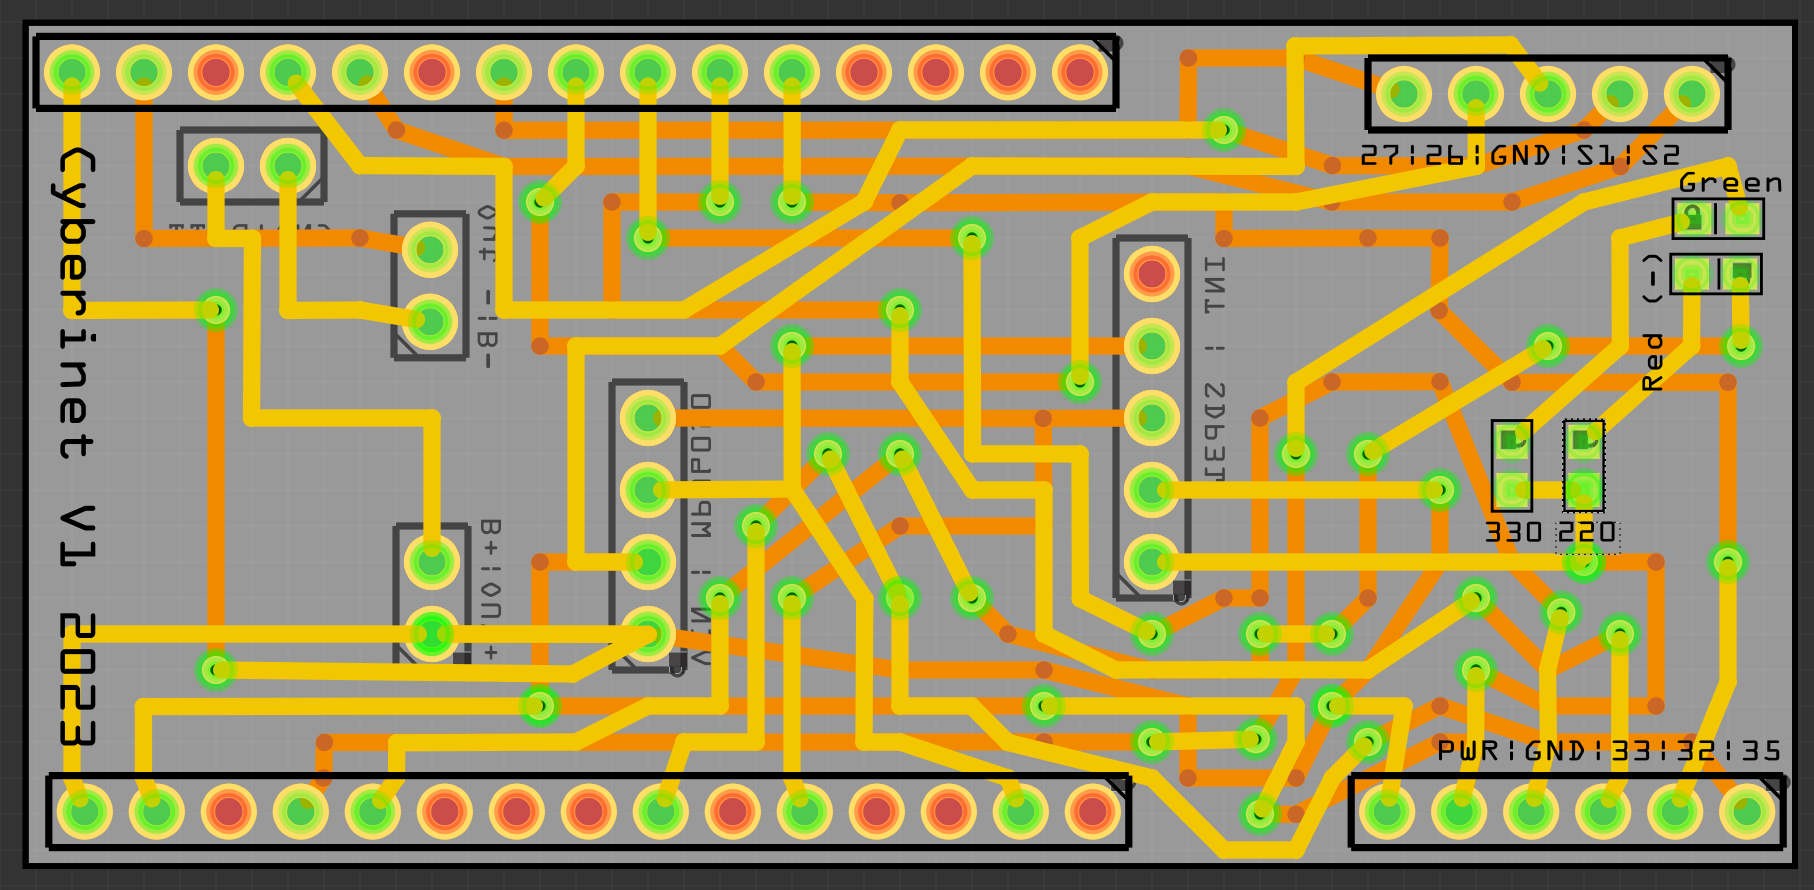
\includegraphics[scale=0.3]{diagrams/PCBs/mainBoard.png}
    \caption{Cyberinet Main Unit PCB}
    \label{fig:mainPCB}
\end{figure}
\end{center}



\section{OEM Components Detailed Photos}

\begin{center}
    \begin{figure}
        \centering
        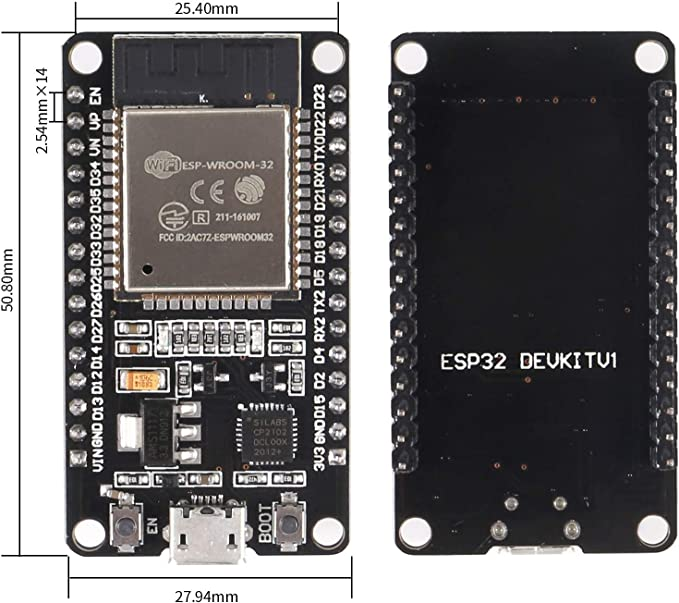
\includegraphics[scale=0.3]{diagrams/oem/esp-32.jpg}
        \caption{ESP-32 DEVKIT V1 Micro-controller}
        \label{fig:ESP-32}
    \end{figure}
\end{center}

\begin{center}
    \begin{figure}
        \centering
        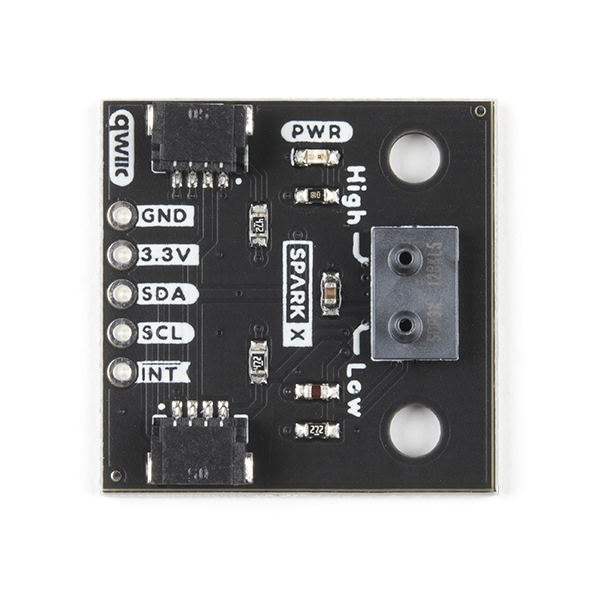
\includegraphics{diagrams/oem/spd31.jpg}
        \caption{Sparkfun SDP-31 Differential Airflow Pressure Qwiic Connect Breakout Board}
        \label{fig:sdp-31}
    \end{figure}
\end{center}


\begin{center}
    \begin{figure}
        \centering
        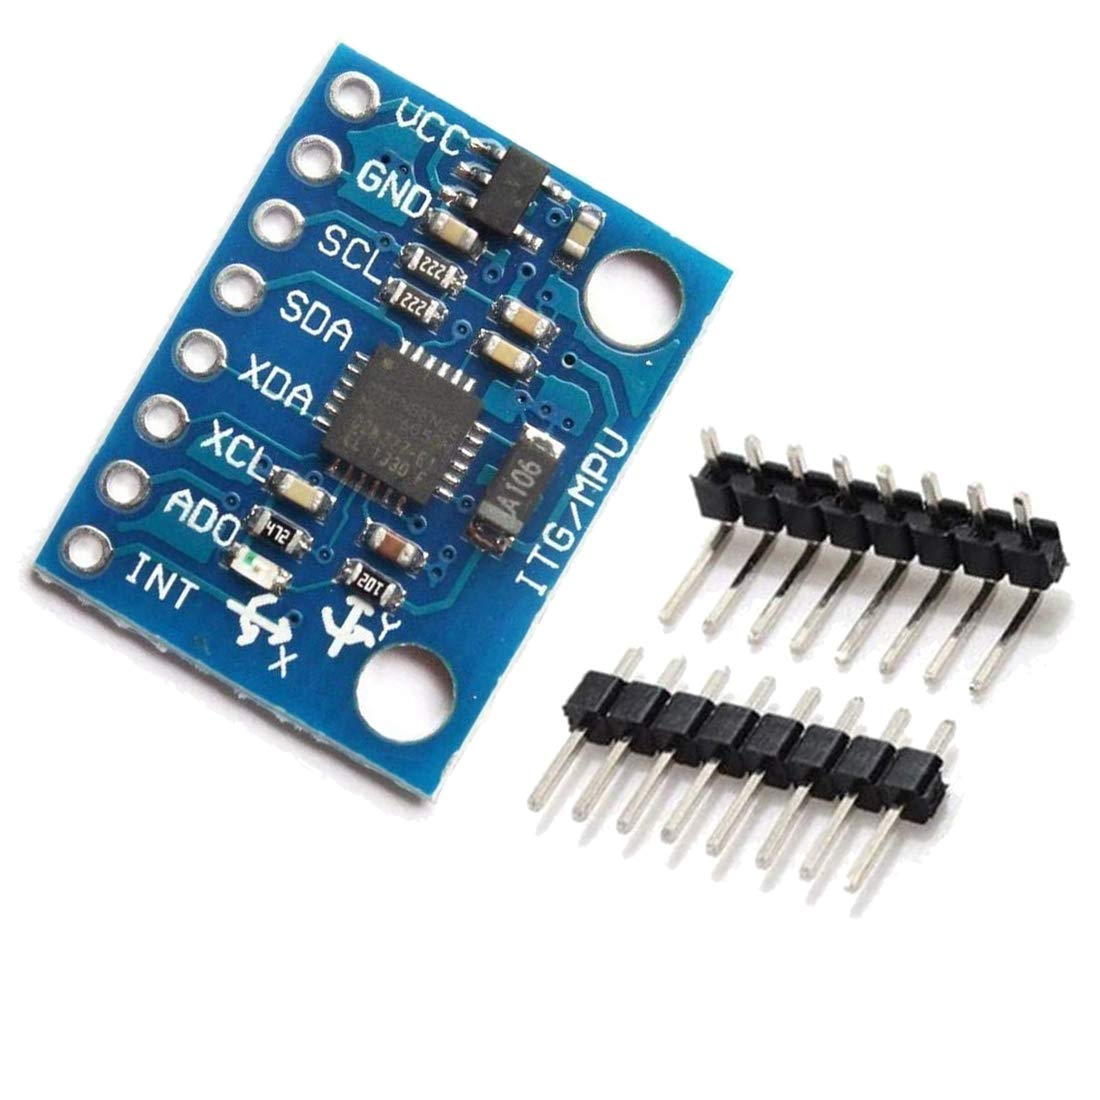
\includegraphics[scale=0.2]{diagrams/oem/6050.jpg}
        \caption{MPU-6050 Gyroscope and Accelerometer}
        \label{fig:6050}
    \end{figure}
\end{center}

\begin{center}
    \begin{figure}
        \centering
        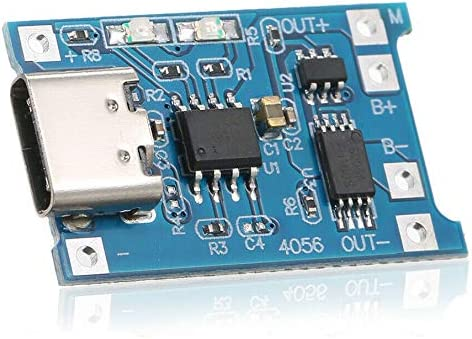
\includegraphics[scale=0.3]{diagrams/oem/4056.jpg}
        \caption{TP-4056 Type C LiPo Battery Charger}
        \label{fig4055}
    \end{figure}
\end{center}




\chapter{Cyberinet Software Components}
This appendix contains all of the Arduino code flashed to the Cyberinet. (Version 1.3), as well as screenshots of the various max patches and objects included in the software bundle.

\section{Arduino .ino Code}

Below is the .ino code that is running on the ESP-32 micro-controller. This code was developed using the Arduino IDE and coding language.

\begin{verbatim}

/*
    Micro Controller Code for the Cyberinet Version 1.3
   Code designed for the ESP-32 WROOM DEVKIT V1 in the Arduino IDE.
   All Serial Communications are over Bluetooth.
   Code may be used or reworked with Attribution. 
   Altering code present on Cyberinet unit is not recommended.
   Code and Other Matierials for the Cyberinet can be found at 
   https://github.com/mbardin/Cyberinet
   Code and Other Marerials made by 
   Matthew A. Bardin [2023] (https://matthewbardin.com)
*/

//libraries to include
#include <SparkFun_SDP3x_Arduino_Library.h>
#include<Wire.h>
#include <BluetoothSerial.h>
#include <MPU6050.h>


// create instances of the libraries above
BluetoothSerial SerialBT;
MPU6050 mpu;
SDP3X airFlow; // constant sensing is on I2C address 0x21


// Global Variables
// dedicated pins
const int pwrLED = 2; // green 330 Ohm
const int msgLED = 4; // red 220 Ohm
const int button1 = 12;
const int button2 = 14;
const int b1LED = 26;
const int b2LED = 27;

// MPU 6050 values
// I2C address of the MPU-6050
const int MPU_ADDR = 0x68; 
// values for 6050
int16_t AcX, AcY, AcZ, GyX, GyY, GyZ; 
// store mapped values for transmitting
float rotX, rotY, rotZ, gForceX, gForceY, gForceZ;


// stores current button state
int button1State = 1;
int button2State = 1;

// store SDP31 values for transmitting
//float diffPressure = 0.0;
//float temperature = 0.0;

void setup() {
  // Pin mode assignment
  pinMode(pwrLED, OUTPUT);
  pinMode(msgLED, OUTPUT);
  // use ESP32's built in pullup resistors
  pinMode(button1, INPUT_PULLUP); 
  pinMode(button2, INPUT_PULLUP);

  Serial.begin(115200);
  // Device name. no spaces or punctuation
  SerialBT.begin("CyberinetV13"); 
  delay(1000); // pause before checking
  
  // various startup and checks
  gyroStartup();
  airflowStartup();
  // device must be restarted if optional expansions are added
  // if everything clears
  startLights();
}

void loop() { // check the sensors and transmit each loop.
  get6050();
  getButtons();
  getAir(); // put 6050 and sdp31 on ends of sensor checks
}

void get6050() {

  ////////////Collect Data
  Wire.beginTransmission(MPU_ADDR);
  Wire.write(0x3B);  // wake up device
  Wire.endTransmission(true);

  Wire.requestFrom(MPU_ADDR, 6); //Request Accel Registers (3B - 40)
  while (Wire.available() < 6);
  // operator first bitshifts the sensor value by 8 bits,
  // then does a bitwise OR to compare to raw data.
  // end result is a combined original and bitshift.
  AcX = Wire.read() << 8 | Wire.read(); 
  AcY = Wire.read() << 8 | Wire.read(); 
  AcZ = Wire.read() << 8 | Wire.read(); 

  Wire.beginTransmission(MPU_ADDR); //I2C address of the MPU
  Wire.write(0x43); //Starting register for Gyro Readings
  Wire.endTransmission();
  Wire.requestFrom(MPU_ADDR, 6); //Request Gyro/Accel Registers (43 - 48)
  while (Wire.available() < 6);
  GyX = Wire.read() << 8 | Wire.read();
  GyY = Wire.read() << 8 | Wire.read();
  GyZ = Wire.read() << 8 | Wire.read();


  ////////////Format Data
  // gravity and rotation offsets
  rotX = GyX *  0.007633587786; 
  rotY = GyY *  0.007633587786;
  rotZ = GyZ *  0.007633587786;

  gForceX = AcX * 0.00006103515;
  gForceY = AcY * 0.00006103515;
  gForceZ = AcZ * 0.00006103515;


  ////////////Transmit Data
  // turn on LED when when transmitting
  digitalWrite(msgLED, HIGH); 
  SerialBT.print("GyroX "); // label
  SerialBT.println(rotX); // value

  SerialBT.print("GyroY "); // label
  SerialBT.println(rotY); // value

  SerialBT.print("GyroZ "); // etc.
  SerialBT.println(rotZ);

  SerialBT.print("AccelX ");
  SerialBT.println(gForceX);

  SerialBT.print("AccelY ");
  SerialBT.println(gForceY);

  SerialBT.print("AccelZ ");
  SerialBT.println(gForceZ);
  digitalWrite(msgLED, LOW);
  // turn off led when done transmitting
}

void getButtons() {
  ////////////Collect Data
  button1State = digitalRead(button1);
  button2State = digitalRead(button2);

  ////////////Transmit Data 
  // turn LED on when tranmitting data
  digitalWrite(msgLED, HIGH); 
  SerialBT.print("B1 "); // label
  SerialBT.println(button1State); // value
  // on-board led state matches button state
  digitalWrite(b1LED, button1State); 
  // repeat for other button
  SerialBT.print("B2 ");
  SerialBT.println(button2State);
  digitalWrite(b1LED, button2State);
  digitalWrite(msgLED, LOW); 
  // turn off led when done transmitting
}

void getAir() {
  ////////////Collect Data

  float diffPressure; 
  float temperature; 
  airFlow.readMeasurement(&diffPressure, &temperature);

  ////////////Transmit Data
  digitalWrite(msgLED, HIGH); 
  SerialBT.print(F("AirP ")); // lebel
  SerialBT.println(diffPressure, 2); // value

  SerialBT.print(F("Temp "));
  SerialBT.println(temperature, 2);
  digitalWrite(msgLED, LOW); 
}


// startup functions
void gyroStartup() {
  Wire.begin(21, 22, 100000); // sda, scl, clock speed
  Wire.beginTransmission(MPU_ADDR);
  Wire.write(0x6B);  // PWR_MGMT_1 register
  Wire.write(0);     // (wakes up the MPU−6050)
  Wire.endTransmission(true);
  SerialBT.println("MPU-6050 Setup Complete");
}

void airflowStartup() {
  // Initialize sensor. Stops if connection cannot be made
  airFlow.stopContinuousMeasurement();

  if (airFlow.begin() == false)
  {
    SerialBT.println(F("SDP31 not detected. Check connections. Freezing..."));
    while (1);
  }
// set to continuous measurement mode
  airFlow.startContinuousMeasurement(true, true);
  SerialBT.println("SDP31 Setup Complete");
}

void startLights() { /
  // process takes 3.5 seconds
  digitalWrite(pwrLED, HIGH);
  digitalWrite(msgLED, HIGH);
  delay(500);
  digitalWrite(msgLED, LOW);
  delay(500);
  digitalWrite(msgLED, HIGH);
  delay(500);
  digitalWrite(msgLED, LOW);
  delay(1000);
  digitalWrite(msgLED, HIGH);
  delay(1000);
  digitalWrite(msgLED, LOW);
}

\end{verbatim}

\section{Max Objects}
This section discusses each of the CNET objects that were created with the intention of interfacing with the Cyberinet. With the exception of CNET.receive, these are smaller objects designed to easily implement the Cyberinet into some of the common audio effects the user is likely already implementing in Max. Because of how CNET.receive works, these objects are not required to utilize the Cyberinet, but are recommended for people learning how to work with Max or the Cyberinet for the first time.

\subsection{Functional Objects}
These objects serve to increase the functionality of the Cyberinet and do not alter sound sources or control other objects.

\subsubsection{CNET.receive}
This is the only required object in the CNET collection. This object is responsible for setting up communications with the Cyberinet, parsing the data, and outputting it to the various outlets. Each sensor on the Cyberinet has a dedicated outlet, so connecting to each outlet will always relay the same sensor. The outlet order is given below.

\begin{enumerate}
    \item GyroX
    \item GyroY
    \item GyroZ
    \item AccelX
    \item AccelY
    \item AccelZ
    \item B1
    \item B2
    \item AirP
    \item Temp
    \item Exp
    \item errorMsg
\end{enumerate}

The final outlet will output an error indicating that CNET received a message it did not recognize, as well as the error causing message.

To establish communications, bangs and toggles are utilized in order to simplify the interface. The user inputs a bang to the first inlet to start the script and list the available ports. When paired to the computer via Bluetooth, the Cyberinet will appear on the list of available ports. The user can then set the port by filling in the message box connected to inlet 2, and receive communications with a bang to the third inlet. Inlet 4 will stop all communications. The process will have to be repeated to initialize them again, and a bang to inlet 5 will install necessary node package manager dependencies and drivers the first time a computer is utilizing the Cyberinet.

The Node script and functionality comes from a package created by the LSU Experimental Music \& Digital Media department, and the JavaScript code for this is shown below in its entirety.

\begin{verbatim}
// EMDM Serial communications in Max
const path = require('path');
const Max = require('max-api');

const { SerialPort, ReadlineParser } = require('serialport')
const baud = 115200;
let devicePort = '/dev/tty-CyberinetV13'

// Create a port
let port;
let availablePorts;
let parser = new ReadlineParser();

// This will be printed directly to the Max console
Max.post(`Loaded the ${path.basename(__filename)} script`);

// Use the 'addHandler' function to register a function for a particular message
Max.addHandler("bang", () => {
	Max.post("Who you think you bangin'?");
});

// Use the 'outlet' function to send messages out of node.script's outlet
Max.addHandler("echo", (msg) => {
	Max.outlet(msg);
});

Max.addHandler("portlist", () => {
  SerialPort.list().then((ports)=>{
    Max.post("Ports: ", ports);
    console.log(ports);
    availablePorts = ports;
  });
});

Max.addHandler('setPort', (port) => {
  devicePort = port;
})

Max.addHandler('open', () => {
  port = new SerialPort({
    path: devicePort,
    baudRate: baud,
  }, function (err) {
    if (err) {
      return console.log('Error: ', err.message)
    }
  })
})

Max.addHandler('enable', () => {
  Max.post('Serial Receive Enabled');

  port.pipe(parser)
  parser.on('data', (cyberData)=>{
    let cyber = cyberData.split(" ");
    let sensor = cyber[0];
    let value = parseFloat(cyber[1]);
    Max.outlet(sensor, value);
  })
})

Max.addHandler('send', (data) => {
  port.write(data, function(err) {
    if (err) {
      return console.log('Error on write: ', err.message)
    }
    console.log('message written')
  })
})
\end{verbatim}

In short, after setting up the port communications, this code will identify the label:value pair and output them separated by a space via the outlet in the Node object. From there, a Max route object separates the values to different outlets based on the labels shown above. Values are scaled to fit a range of 0-1 where appropriate.

\subsubsection{CNET.rangeSet}
Used for adjusting the value scaling within CNET.receive. This object is used to fine tune the ranges expected for a performer with their Cyberinet unit. Maximum and minimum sensor values can be determined by looking at the Max terminal when the raw outputs are being displayed. Ranges are set to a specific sensor utilizing the same labels as those used in CNET.receive. Setting the sensor label with a message or sending a bang to the first outlet will trigger a list to be output from this object.

Within CNET.receive, an additional route and a handful of unpack objects are used to properly apply the data. All values leaving CNET.receive are still mapped to a range of 0-1 after this new scaling occurs.

\subsubsection{CNET.latency}
Used to calculate the latency between the Cyberinet detecting a sensor value change on the hardware, and that change being reflected in the Max environment. To achieve this, a microphone is needed. 

To test the latency, first you must connect the Cyberinet using CNET.receive, and ensure that the Button expansion is connected. 

Using the patch, a sound file is recorded. One channel of the stereo file records the sound of a button clicking on the Cyberinet. This button press is used to generate a pulse of white noise on the second channel.

The recordings are then compared to determine the time between the real-world action and the software response which is represented in milliseconds for the user. Large objects located between the computer and the Cyberinet may negatively affect the latency.

\subsubsection{CNET.tuner}

This object is a simple tuner based off of the one included in the RNBO max collection. It receives a signal from an external microphone and outputs both the pitch and frequency of the sound. In this version of the Cyberinet, it must be located in the Max software as the ESP-32's ADC's are not powerful enough to run a tuner along with everything else. It is recommended for both tuning purposes, as well as pitch identification purposes. 

An incoming signal is analyzed for pitch content, and the results are given through the outlets in the bottom of the object. The pitch output is recommended for tuning purposes, and the specific frequency output is recommended for use in calculations and processing. A graphic representation is also given for the pitch which can be viewed by opening CNET.tuner inside of a bpatcher object. 

\subsubsection{CNET.pan}
I was unsure about which section to place this object in. I chose its ultimate placement here as the object is not directly changing the sound, but rather it receives data to control the stereo panning of a signal.

\subsubsection{CNET.dmx}
This object functions to allow the Cyberinet to control DMX lighting with its various sensors. Note that this will not work with every DMX controller, and is specifically designed to interface with the Chauvet DMX-AN 2. After being setup with the desired environmental settings, CNET.dmx takes in three sensor readings to control the red, green, and blue levels of the connected lights.

\subsection{Audio Effects}
These audio effects are designed to receive information from the functional objects above and utilize the data to either process sound or control another object. Generally, these effects are relatively simple alterations of sounds similar to audio effects found in most DAW's.

\subsubsection{CNET.reverb}
This is a stereo Schroder reverb. Type more here about the effect. Include how it works, the parameters that can be controlled, and anything unique about it. Finish with sceenshots of the main patch and gen patches.

\subsubsection{CNET.compressor}
CNET.compressor is a fairly standard compressor that is able to receive data from the Cyberinet in order to control the threshold, ratio, attack, release, and gain staging before and after the effect. By connecting a meter~ object to the last outlet, a faux VU meter can be created to show the gain reduction happening in the compressor.

One unique feature of this compressor is that it takes in a mono signal and outputs a stereo signal.

\subsubsection{Various Delays}
A total of four various delays have been created for a variety of different audio effects. these include:

\begin{itemize}
    \item CNET.delay: a simple delay of an audio signal. The specific delay time can be controlled by 
    \item CNET.feedbackDelay: a delay with an adjustable feedback percentage
    \item CNET.multDelay: a delay with four individually controllable delay lines
    \item CNET.vibDelay: a delay line that also creates a vibrato effect on the delayed signal.
\end{itemize}

\subsubsection{CNET.karplusStrong}
This patch works by taking the incoming audio signal as a sample. When triggered, the algorithm generates a plucked-string sound utilizing this source signal. The end result is a pluck sound that will match up with the incoming sounds, and can be triggered on-demand. The filter coefficient, approximate pitch of the resulting 'pluck', and the effect's output volume are all controlled with the Cyberinet.


% make sure most up-to-date pdf is shown here
\chapter{Puzzle of a Park Full Score}

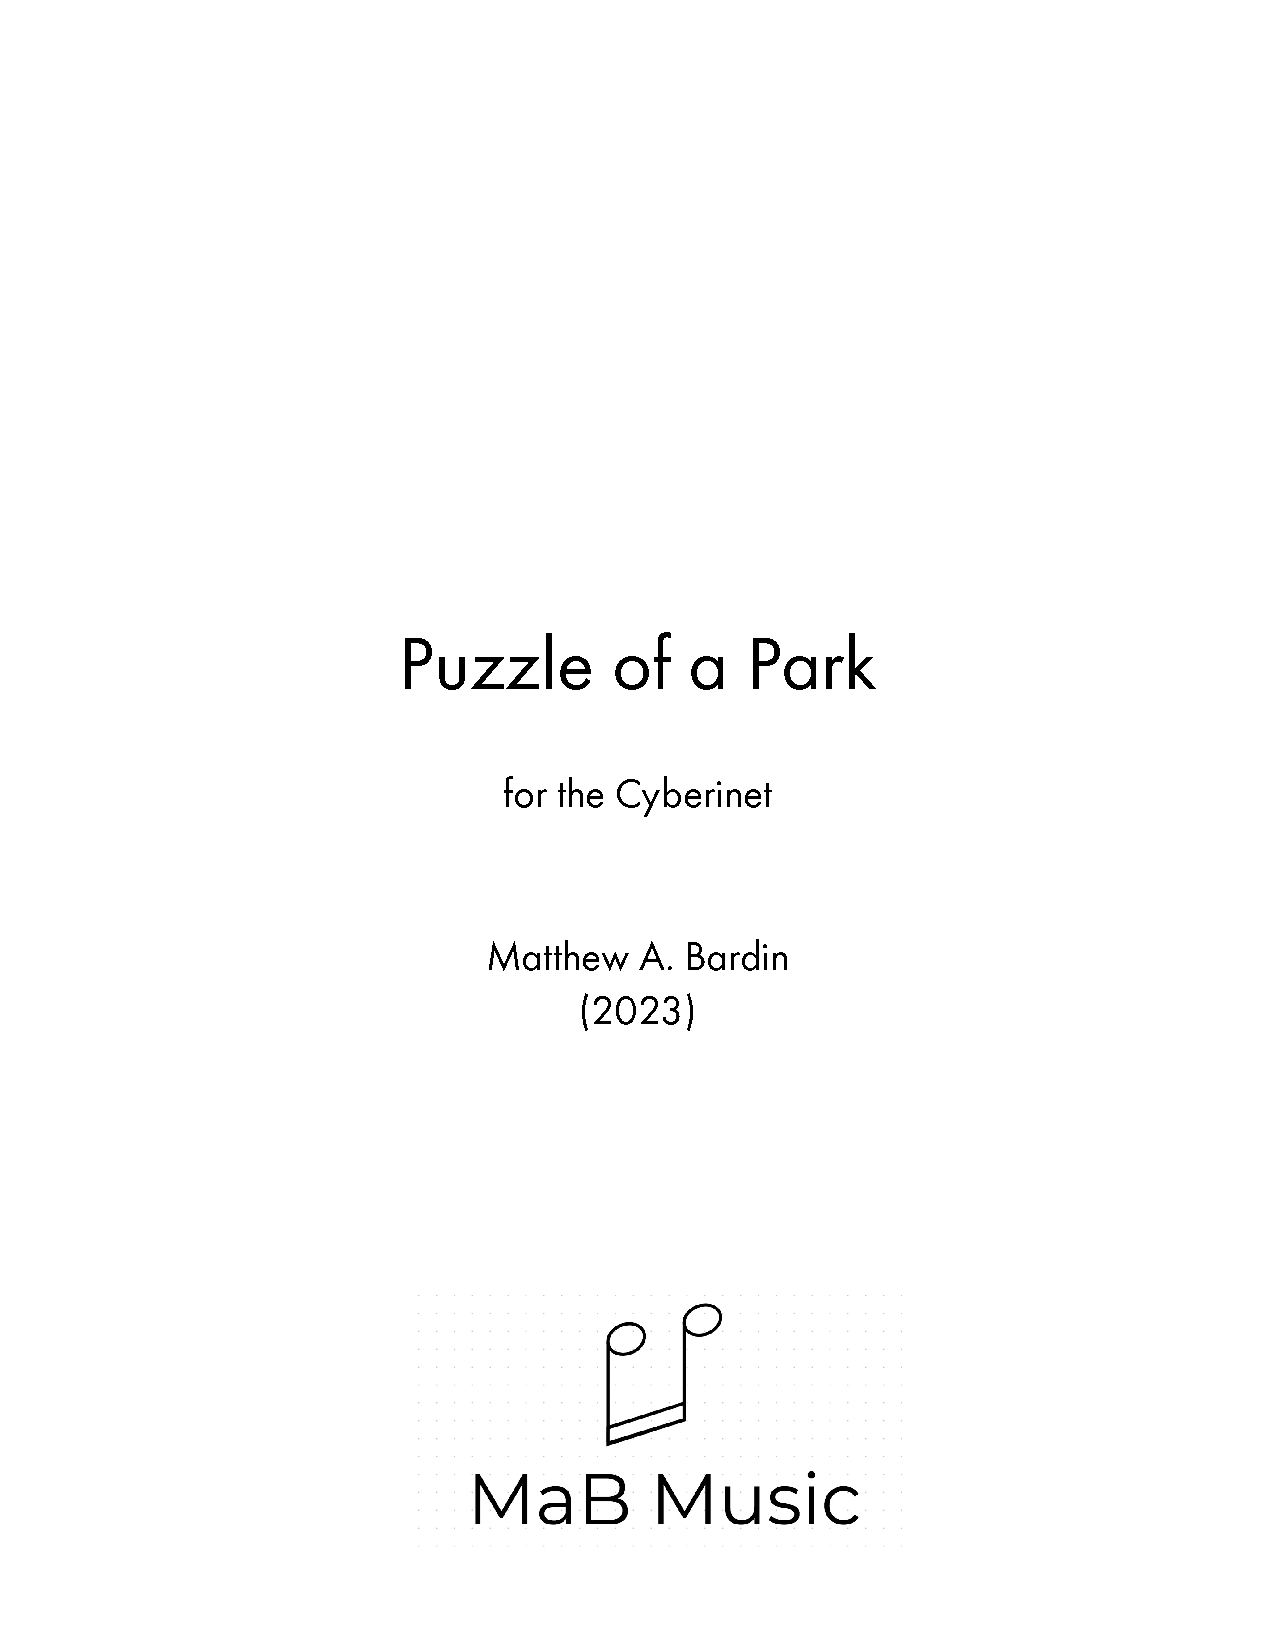
\includepdf[pages=1-17]{Scores/PPFull.pdf}

\chapter{Ethereal Presence Full Score}

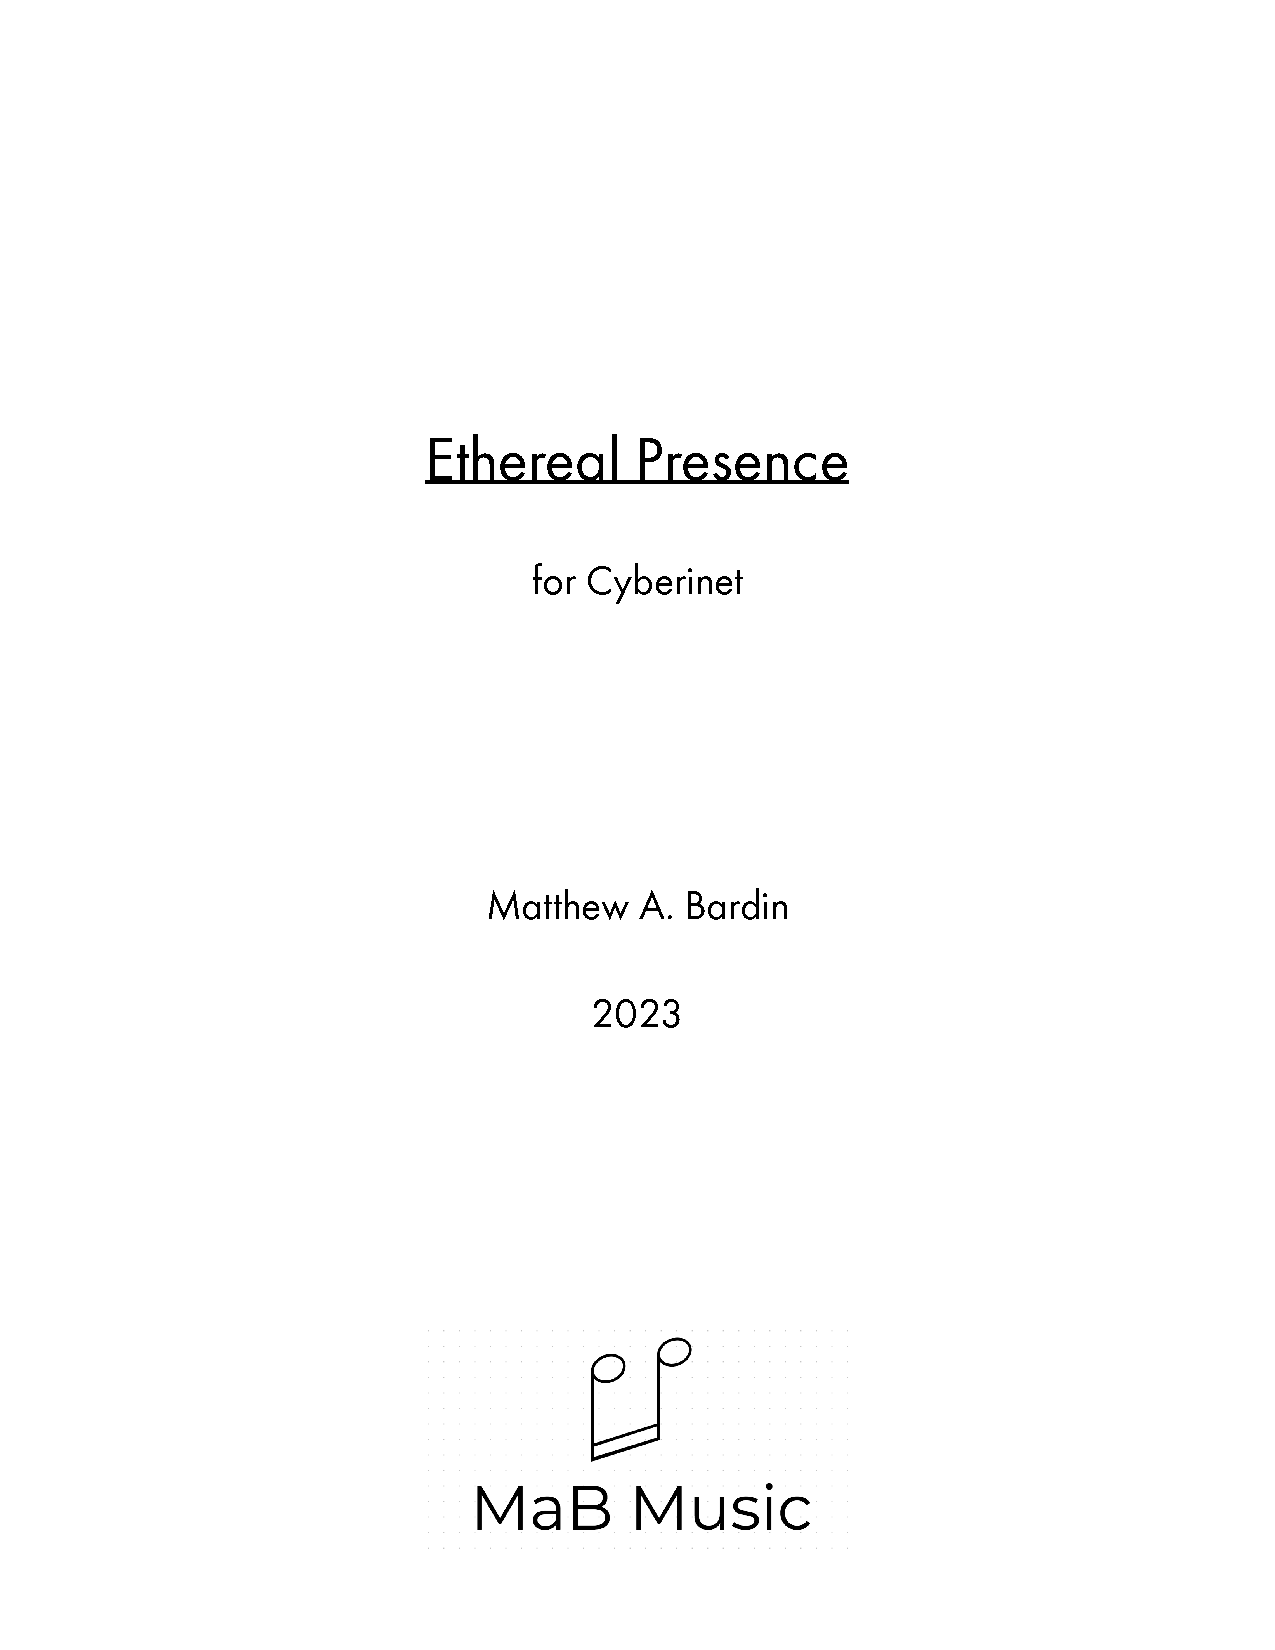
\includepdf[pages=1-9]{Scores/EP.pdf}

\chapter{Raindrops on a Tin Roof}

\section{Full Score}

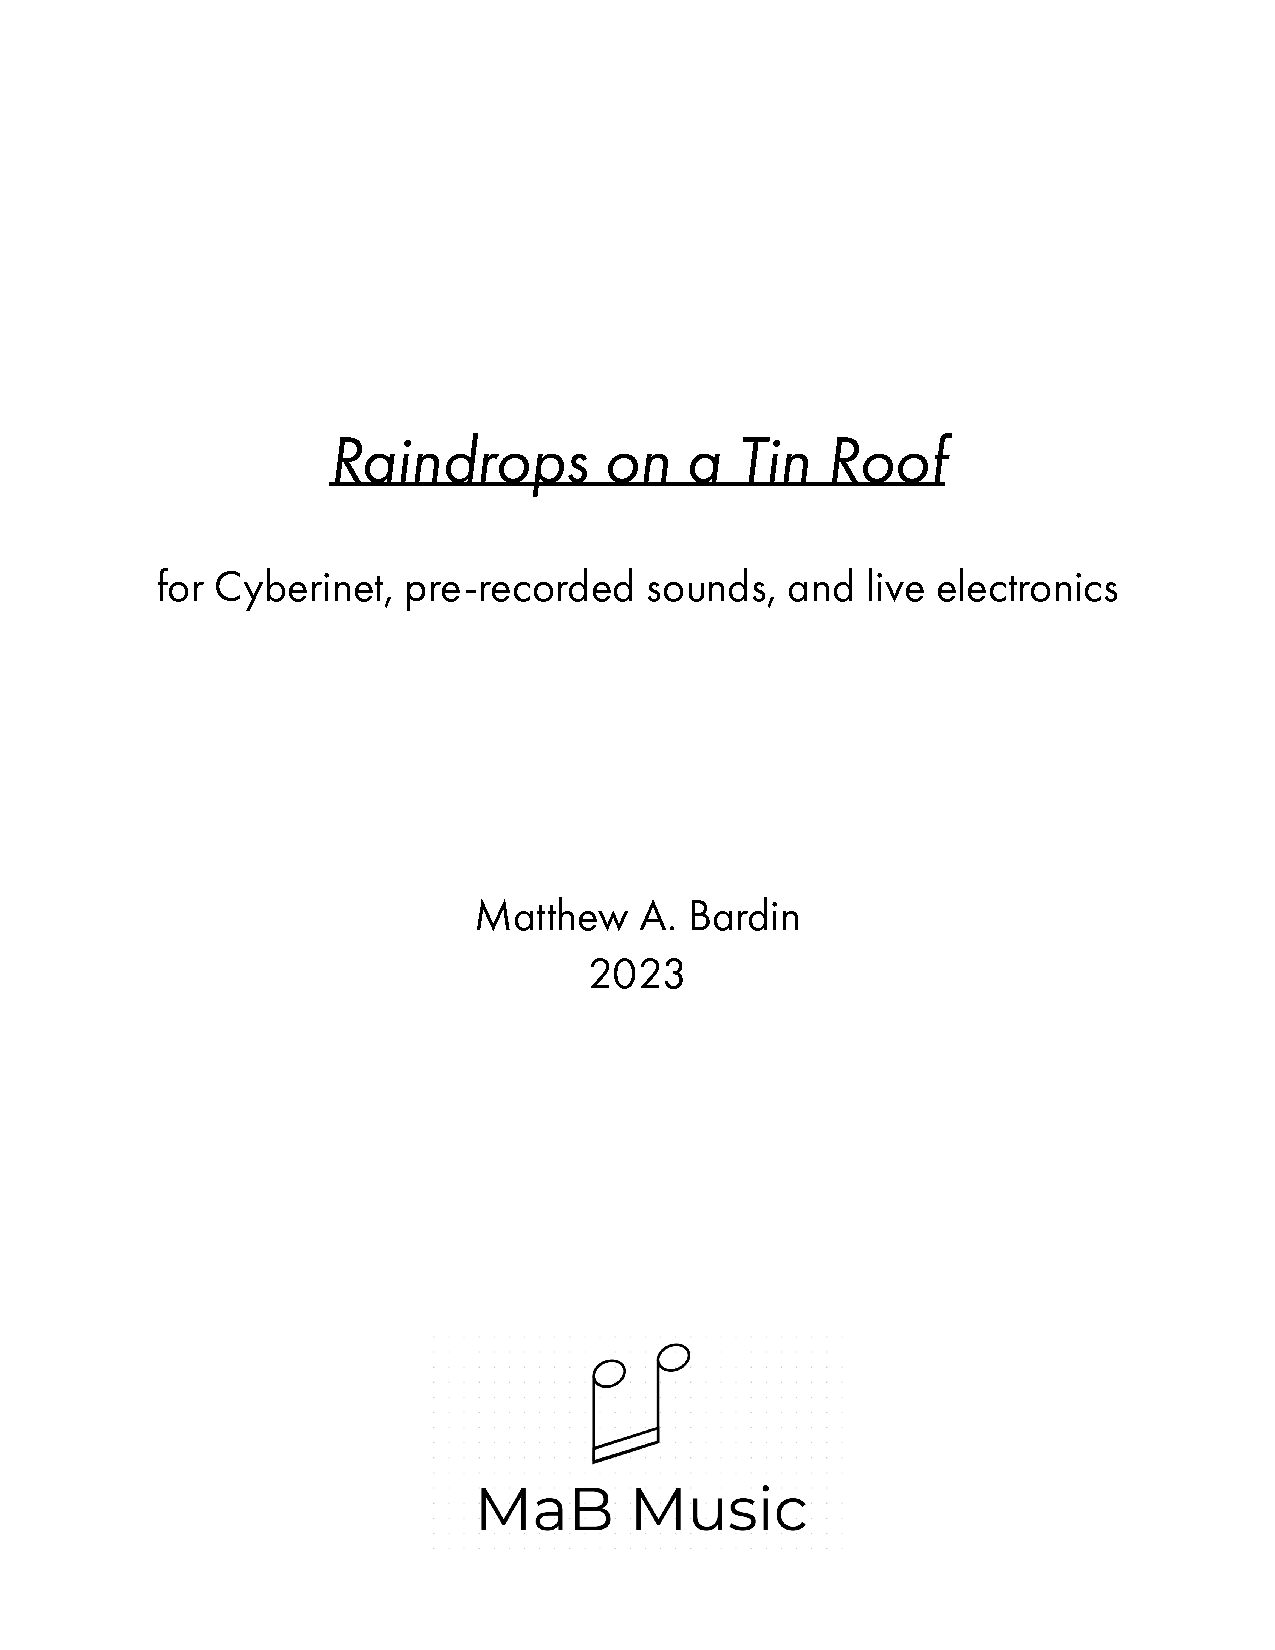
\includepdf[pages=1-21]{Scores/raindrops.pdf} 
%  list page range and file location

\section{Short Story Text}

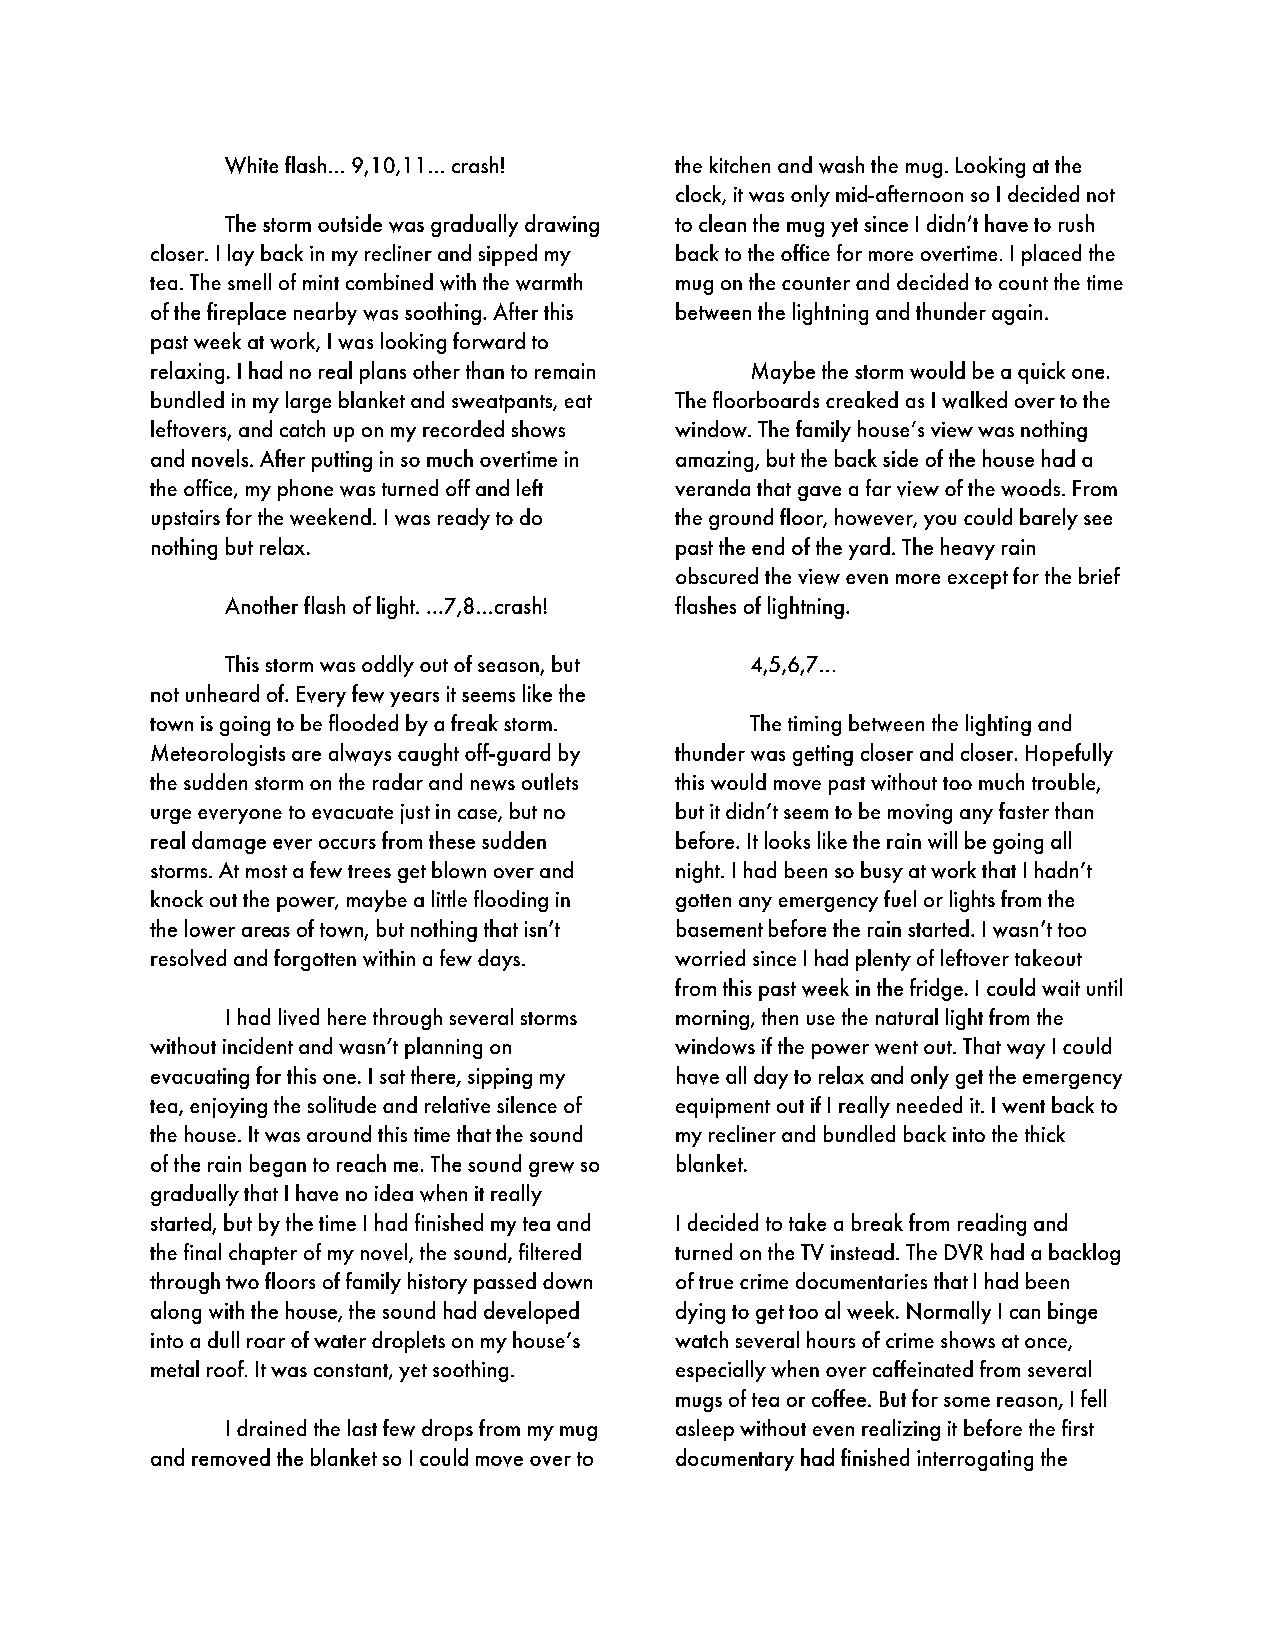
\includepdf[pages=1-4]{Scores/Raindrops Text.pdf}



% \chapter{Permissions}

% The ``permissions'' area reproduces requests and permissions for previously published material or material belonging to others. If included, then it should be the last appendix.


%% After ``\backmatter'', subsequent \chapter commands produce
%% unnumbered headings.
\backmatter


\begin{thebibliography}{99} % double check the formatting for the EMDM citations. Include template in comments here

% \bibitem{label}

\bibitem{puzzleScore} Bardin, Matthew. \emph{Puzzle of a Park} Performance Score, MaBMusic, 2023.

\bibitem{EPScore} Bardin, Matthew. \emph{Ethereal Presence} Performance Score, MaBMusic, 2023.

\bibitem{Raindrops Score} Bardin, Matthew. \emph{Raindrops on a Tin Roof} Performance Score, MaBMusic, 2023.

\bibitem{Raindrops Score} Bardin, Matthew. \emph{Raindrops on a Tin Roof} Short Story, Kindle Direct Publishing, 2022.

\bibitem{gelbBodyLearning2013} Gelb, Michael. \emph{Body Learning: An Introduction to the Alexander Technique} Updated 40th Anniversary Edition. Aurum Publishing, 2013.

\bibitem{gordosOliverosCybernetics} Gordon, Theodore. \emph{'Androgynous Music': Pauline Oliveros's Early Cybernetic Improvisation}, Contemporary Music Review Vol. 40 Issue 4, 2022.

\bibitem{HolmesElectronicMusic2020} Holmes, Thom. \emph{Electronic and Experimental Music: Technology, Music and Culture, 6th Edition}. Routledge/Taylor \& Francis Group, 2020. 

\bibitem{cyberneticsScoreSite} Lucarelli, Fosco. \emph{Roland Kayn and the Development of Cybernetic Music}, Socks Studio, \url{https://socks-studio.com/2014/11/03/roland-kayn-and-the-development-of-cybernetic-music/}. 11/03/2013. Accessed 04/10/2023.

\bibitem{miranda_Wanderley_instrumentControl_2006} Miranda, Eduardo and Wanderly, Marcelo. \emph{New Digital Musical Instruments: Control and Interaction Beyond the Keyboard} Computer Music and Digital Audio Series, A-R Editions, Inc., 2006.

\bibitem{reid2016} Reid, Sarah and Gaston, Ryan and Honigman, Colin and Kapur, Ajay. \emph{Minimally Invasive Gesture Sensing Interface (MIGSI) for Trumpet}, Proceedings of the International Conference on New Interfaces for Musical Expression, 2016.

\bibitem{rolandKaynBio} Ricci, Massimo. \emph{Roland Kayn: Biography}, \url{https://kayn.nl/biography/}. Accessed 04/15/2023.

\bibitem{Schiesser2012} Schiesser, S{\'e}bastien and Schacher, Jan C. \emph{SABRe: The Augmented Bass Clarinet}, Proceedings of the International Conference on New Interfaces for Musical Expression, 2012.

\bibitem{cultureandHumanity2002} Oliveros, Pauline. Edited by Tong, Kwok Siu and Sin-wai, Chan. \emph{Culture and Humanity in the New Millennium: The Future of Human Values} Chinese University Press 2002

\bibitem{WeinerCybernetics2019} Weiner, Norbert. \emph{Cybernetics or Control and Communication in the Animal and the Machine}, MIT Press, 2019

% look at a way to make this better. I HATE how the template is handling references.


% \bibitem{mathIntoLatex} George Gr\"{a}tzer,
% {\em Math into \LaTeX: an introduction to LaTeX and AMS-LaTeX, Third Edition},
% Library of Congress, Boston, 2000.

\end{thebibliography}


\chapter{Vita}

Matthew Bardin, originally a native of Central Florida, is currently based in Baton Rouge, and has written music for large ensembles, chamber groups, voice, solo instruments, and electronics. He holds a Master of Music from the Boston Conservatory at Berklee, and a  Bachelor of Music from Stetson University. Matthew is currently working towards a Ph.D in Experimental Music \& Digital Media from Louisiana State University. He is currently affiliated with the American Society of Composer, Authors, and Publishers, and his works are often performed by several student soloists and groups throughout the course of the academic year. He also has presented his music at the annual Electric LaTex festival in 2020 and 2022, co-hosted an online workshop at NIME 2020, and served as the 2021 Composer in Residence of the University Presbyterian Church in Baton Rouge, LA. In 2022 he traveled to Edinburgh, Scotland to run audio for the LSU produced show \textit{Dream Logos}; a show for which he also composed the music and sound design. Following this document, Matthew's upcoming projects include a concerto for the Cyberinet, as well as completing a new creative coding textbook.

Matthew has studied with Drs. Manuel deMurga, Sydney Hodkinson, Eun Young Lee, Tina Tallon, and most recently, Drs. Jesse Allison, Edgar Berdhal, and Mara Gibson. Matthew is currently teaching the courses Sound Design, Digital Storytelling, and Programming Digital Media to local dual enrollment students through the LSU STEM Pathways Program. Matthew also trains local teachers in the PDM course material, as well as a shortened version of the course for the LSU Pre-College summer program. He has also written a large portion of the programming course's textbook

\end{document}
